\documentclass[cs4size,a4paper,10pt]{ctexart}   

\linespread{1.5}
\usepackage{geometry}%用于设置上下左右页边距
	\geometry{left=2.5cm,right=2.5cm,top=3.2cm,bottom=2.7cm}
\usepackage{xeCJK,amsmath,paralist,enumerate,booktabs,multirow,graphicx,subfig,setspace,listings,lastpage,hyperref}
\usepackage{amsthm, amssymb, bm, color, framed, graphicx, hyperref, mathrsfs}
\usepackage{mathrsfs}  
	\setlength{\parindent}{2em}
	\lstset{language=Matlab}%
\usepackage{fancyhdr}
\usepackage{graphicx}
\usepackage{subfloat}
\usepackage{listings}
\usepackage{xcolor}
\usepackage{float}
\usepackage{paralist}
\usepackage{setspace}
\usepackage{titlesec}
\usepackage{enumitem}
\usepackage{hyperref}
\usepackage{multirow}
\usepackage{threeparttable}



\hypersetup{
	colorlinks=true,
	linkcolor=black
}

\setenumerate{partopsep=0pt,topsep=0pt}
\setitemize{itemsep=0pt,partopsep=0pt,topsep=0pt}

\titlespacing*{\section}{0pt}{3pt}{3pt}
\titlespacing*{\subsection}{0pt}{2pt}{2pt}
\titlespacing*{\subsubsection}{0pt}{1pt}{1pt}
\titlespacing*{\paragraph}{0pt}{0pt}{0pt}

\ctexset{secnumdepth=4,tocdepth=4}
\setlength{\parindent}{0pt}
\setstretch{1.2}


\setCJKmainfont[BoldFont={FZHei-B01},ItalicFont={FZKai-Z03}]{FZShuSong-Z01} 
\setCJKsansfont[BoldFont={FZHei-B01}]{FZKai-Z03} 
\setCJKmonofont[BoldFont={FZHei-B01}]{FZFangSong-Z02}
\setCJKfamilyfont{zhsong}{FZShuSong-Z01} 
\setCJKfamilyfont{zhhei}{FZHei-B01} 
\setCJKfamilyfont{zhkai}[BoldFont={FZHei-B01}]{FZKai-Z03} 
\setCJKfamilyfont{zhfs}[BoldFont={FZHei-B01}]{FZFangSong-Z02} 
\renewcommand*{\songti}{\CJKfamily{zhsong}} 
\renewcommand*{\heiti}{\CJKfamily{zhhei}} 
\renewcommand*{\kaishu}{\CJKfamily{zhkai}} 
\renewcommand*{\fangsong}{\CJKfamily{zhfs}}


\definecolor{mKeyword}{RGB}{0,0,255}          % bule
\definecolor{mString}{RGB}{160,32,240}        % purple
\definecolor{mComment}{RGB}{34,139,34}        % green
\definecolor{mNumber}{RGB}{128,128,128} 

\lstdefinestyle {njulisting} {
	basewidth = 0.5 em,
	lineskip = 3 pt,
	basicstyle = \small\ttfamily,
	% keywordstyle = \bfseries,
	commentstyle = \itshape\color{gray}, 
	basicstyle=\small\ttfamily,
	keywordstyle={\color{mKeyword}},     % sets color for keywords
	stringstyle={\color{mString}},       % sets color for strings
	commentstyle={\color{mComment}},     % sets color for comments
	numberstyle=\tiny\color{mNumber},
	numbers = left,
	captionpos = t,
	breaklines = true,
	xleftmargin = 2 em,
	xrightmargin = 2 em,
	frame=tlrb,
	tabsize=4
}

\lstset{
style = njulisting, % 调用上述样式 
flexiblecolumns % 允许调整字符宽度
}


%================= 基本格式预置 ===========================
\usepackage{fancyhdr}
\pagestyle{fancy}
\lhead{\textsc{Computer Networking}}
\rhead{第四章\ 网络层}
\cfoot{\thepage}
\renewcommand{\headrulewidth}{0.4pt}
\renewcommand{\theenumi}{(\arabic{enumi})}
\CTEXsetup[format={\bfseries\zihao{-3}}]{section}
\CTEXsetup[format={\bfseries\zihao{4}}]{subsection}
\CTEXsetup[format={\bfseries\zihao{-4}}]{subsubsection}


\renewcommand{\contentsname}{目录}  
\begin{document}

	\begin{center}
		{\huge\textbf{第四章\ 网络层}}
	\end{center}
	%---------目录---------% 
	\pagenumbering{Roman}
	\tableofcontents
	\clearpage

 	%---------正文---------% 
	\pagenumbering{arabic}
	\setcounter{page}{1}
	\setlength{\parskip}{0.65em}

	\section{网络层提供的两种服务}

	\begin{itemize}
		\item 面向连接的虚电路服务
		\begin{itemize}
			\item 可靠通信由网络来保证
			\item 必须建立网络层的连接——虚电路 VC(virtual circuit)
			\item 通信双方沿着已建立的虚电路发送分组
			\item 目的主机的地址仅在连接建立阶段使用,之后每个分组的首部只需携带一条虚电路的编号(构成虚电路的每一段链路都有一个虚电路编号)
			\item 这种通信方式如果再使用可靠传输的网络协议,就可使所发送的分组最终正确到达接收方(无差错按序到达、不丢失、不重复)
			\item 通信结束后,需要释放之前所建立的虚电路
			\item 很多广域分组交换网都使用面向连接的虚电路服务。例如,曾经的 X.25 和逐渐过时的帧中继 FR、异步传输模式 ATM 等
		\end{itemize}
		\item 无连接的数据报服务
		\begin{itemize}
			\item 可靠通信应当由用户主机来保证
			\item 不需要建立网络层连接
			\item 每个分组可走不同的路径
			\item 每个分组的首部必须携带目的主机的完整地址
			\item 这种通信方式所传送的分组可能误码、丢失、重复和失序
			\item 由于网络本身不提供端到端的可靠传输服务,这就使网络中的路由器可以做得比较简单,而且价格低廉(与电信网交换机相比较)
			\item 因特网采用了这种设计思想,也就是将复杂的网络处理功能置于因特网的边缘(用户主机和其内部的运输层),而将相对简单的尽最大努力的分组交付功能置于因特网核心
		\end{itemize}
	\end{itemize}

	\begin{figure}[H]
		\centering
		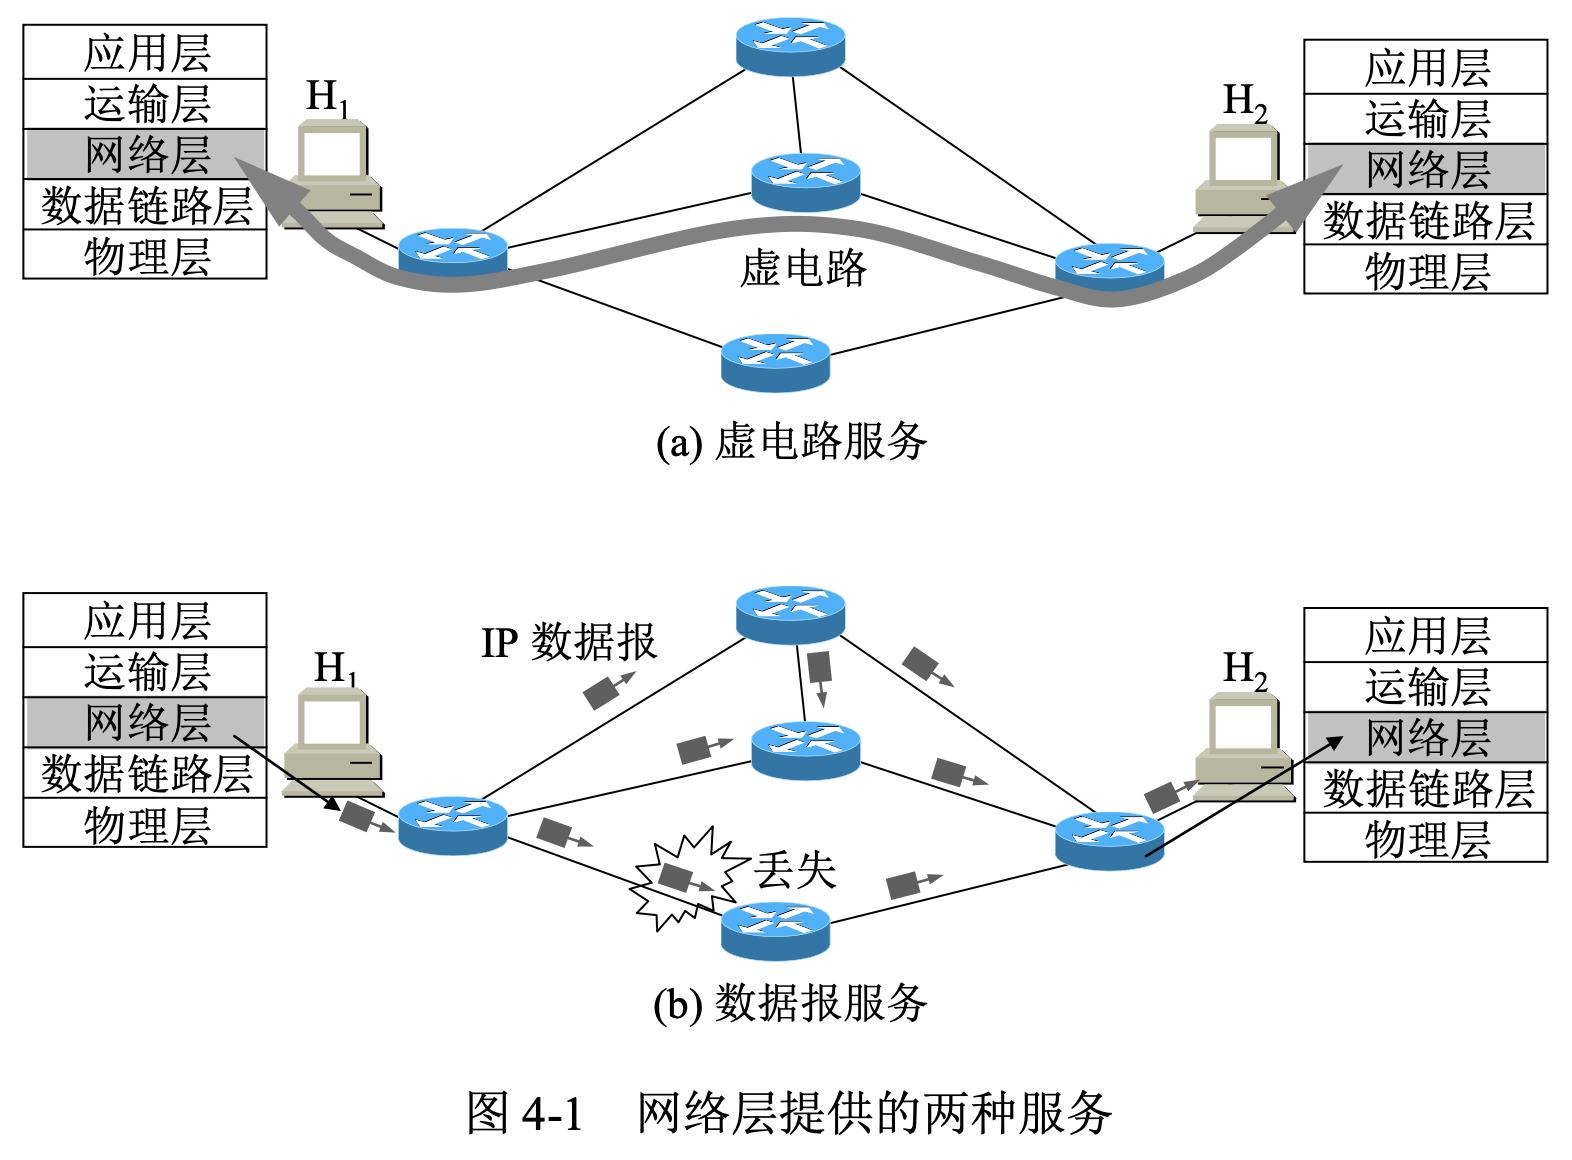
\includegraphics[width=0.6\textwidth]{img/4.1}
	\end{figure}
	
	虚电路服务与数据报功能的比较

	\begin{table}[H]
		\centering
		\resizebox{\linewidth}{!}{
		\begin{tabular}{|c|c|c|}
		\hline
		对比的方面         & 虚电路服务                   & 数据报服务                     \\ \hline
		思路            & 可靠通信应当由网络来保证            & 可靠通信应当由用户主机来保证            \\ \hline
		连接的建立         & 必须建立网络连接                & 不需要建立网络连接                 \\ \hline
		终点地址          & 仅在连接建立阶段使用,每个分组使用短的虚电路号 & 每个分组都有终点的完整地址             \\ \hline
		分组的转发         & 属于同一条虚电路的分组均按照同一路由进行转发  & 每个分组独立选择路由进行转发            \\ \hline
		当结点出故障时       & 所有通过出故障的结点的虚电路均不能工作     & 出故障的结点可能会丢失分组,一些路由可能会发生变化 \\ \hline
		分组的顺序         & 总是按发送顺序到达终点             & 到达终点的时间不一定按发送顺序           \\ \hline
		端到端的差错处理和流量控制 & 可以由网络负责,也可以由用户主机负责      & 由用户主机负责                   \\ \hline
		\end{tabular}
		}
	\end{table}
	
	由于 TCP/IP 体系结构的因特网的网际层提供的是简单灵活的、无连接的、尽最大努力交付的数据报服务,因此本章主要围绕网际层如何传送 IP 数据报这个主题进行讨论

	\section{网际协议IP}
	网际协议 IP 是 TCP/IP 体系中两个最主要的协议之一,与 IP 协议配套使用的还有三个协议
	\begin{itemize}
		\item 地址解析协议 ARP(Address Resolution Protocol)
		\item 网际控制报文协议 ICMP(Internet Control Message Protocol)
		\item 网际组管理协议 IGMP(Internet Group Management Protocol)
	\end{itemize}

	\begin{figure}[H]
		\centering
		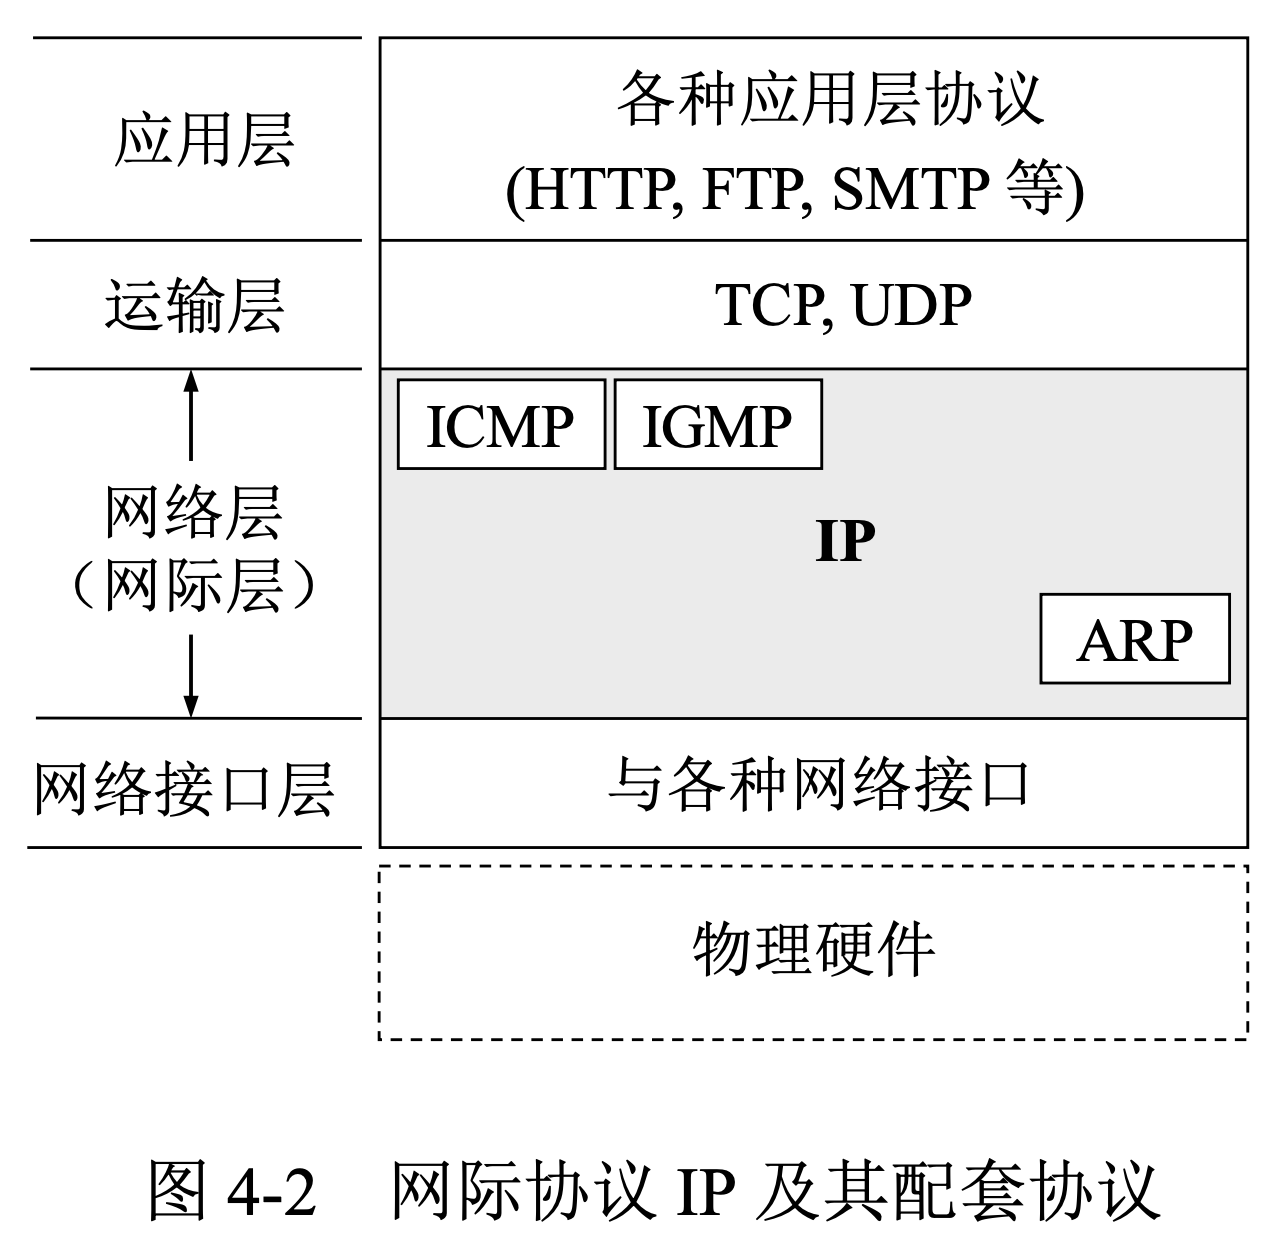
\includegraphics[width=0.45\textwidth]{img/4.2}
	\end{figure}

	\subsection{虚拟互连网络}
	\begin{figure}[H]
		\centering
		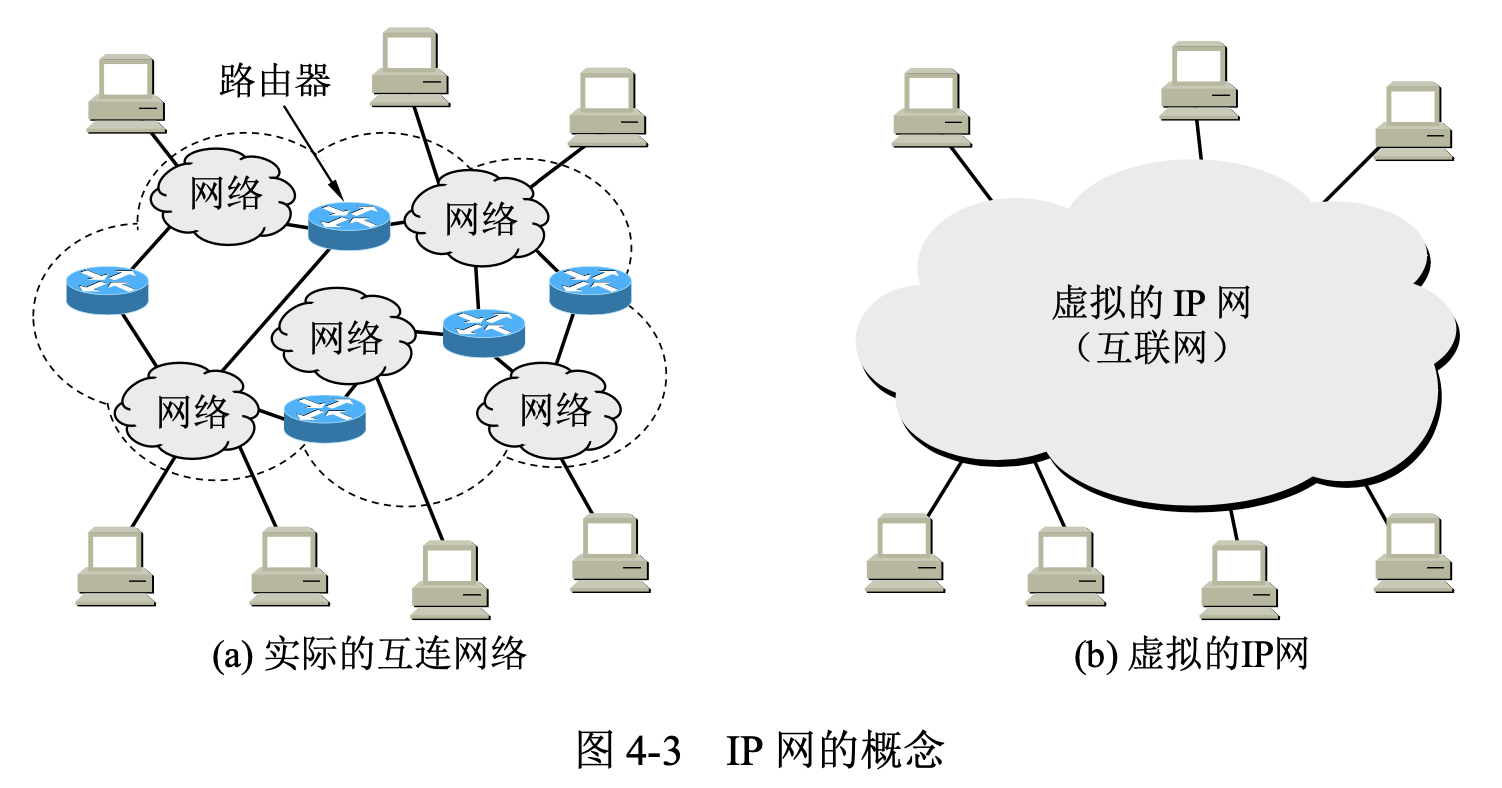
\includegraphics[width=0.65\textwidth]{img/4.3}
	\end{figure}
	\begin{itemize}
		\item 图(a)表示有许多计算机网络通过一些路由器进行互连。由于参加互连的计算机网络都使用相同的网际协议 IP,因此可以把互连以后的计算机网络看成如图(b)所示的一个虚拟互连网络
		\item 虚拟互连网络也就是逻辑互连网络,就是互连起来的各种物理网络的异构性本来是客观存在的,但是我们利用 IP 协议就可以使这些性能各异的网络在网络层上看起来好像是一个统一的网络
		\item 当 IP 网上的主机进行通信时,就好像在一个单个网络上通信一样,它们看不见互连的各网络的具体异构细节
	\end{itemize}

	只从网络层考虑问题,IP 数据报在下图中的传播路径为
	$$H_1 \to R_1 \to R_2 \to R_3 \to R_4 \to R_5 \to H_2$$
	\begin{figure}[H]
		\centering
		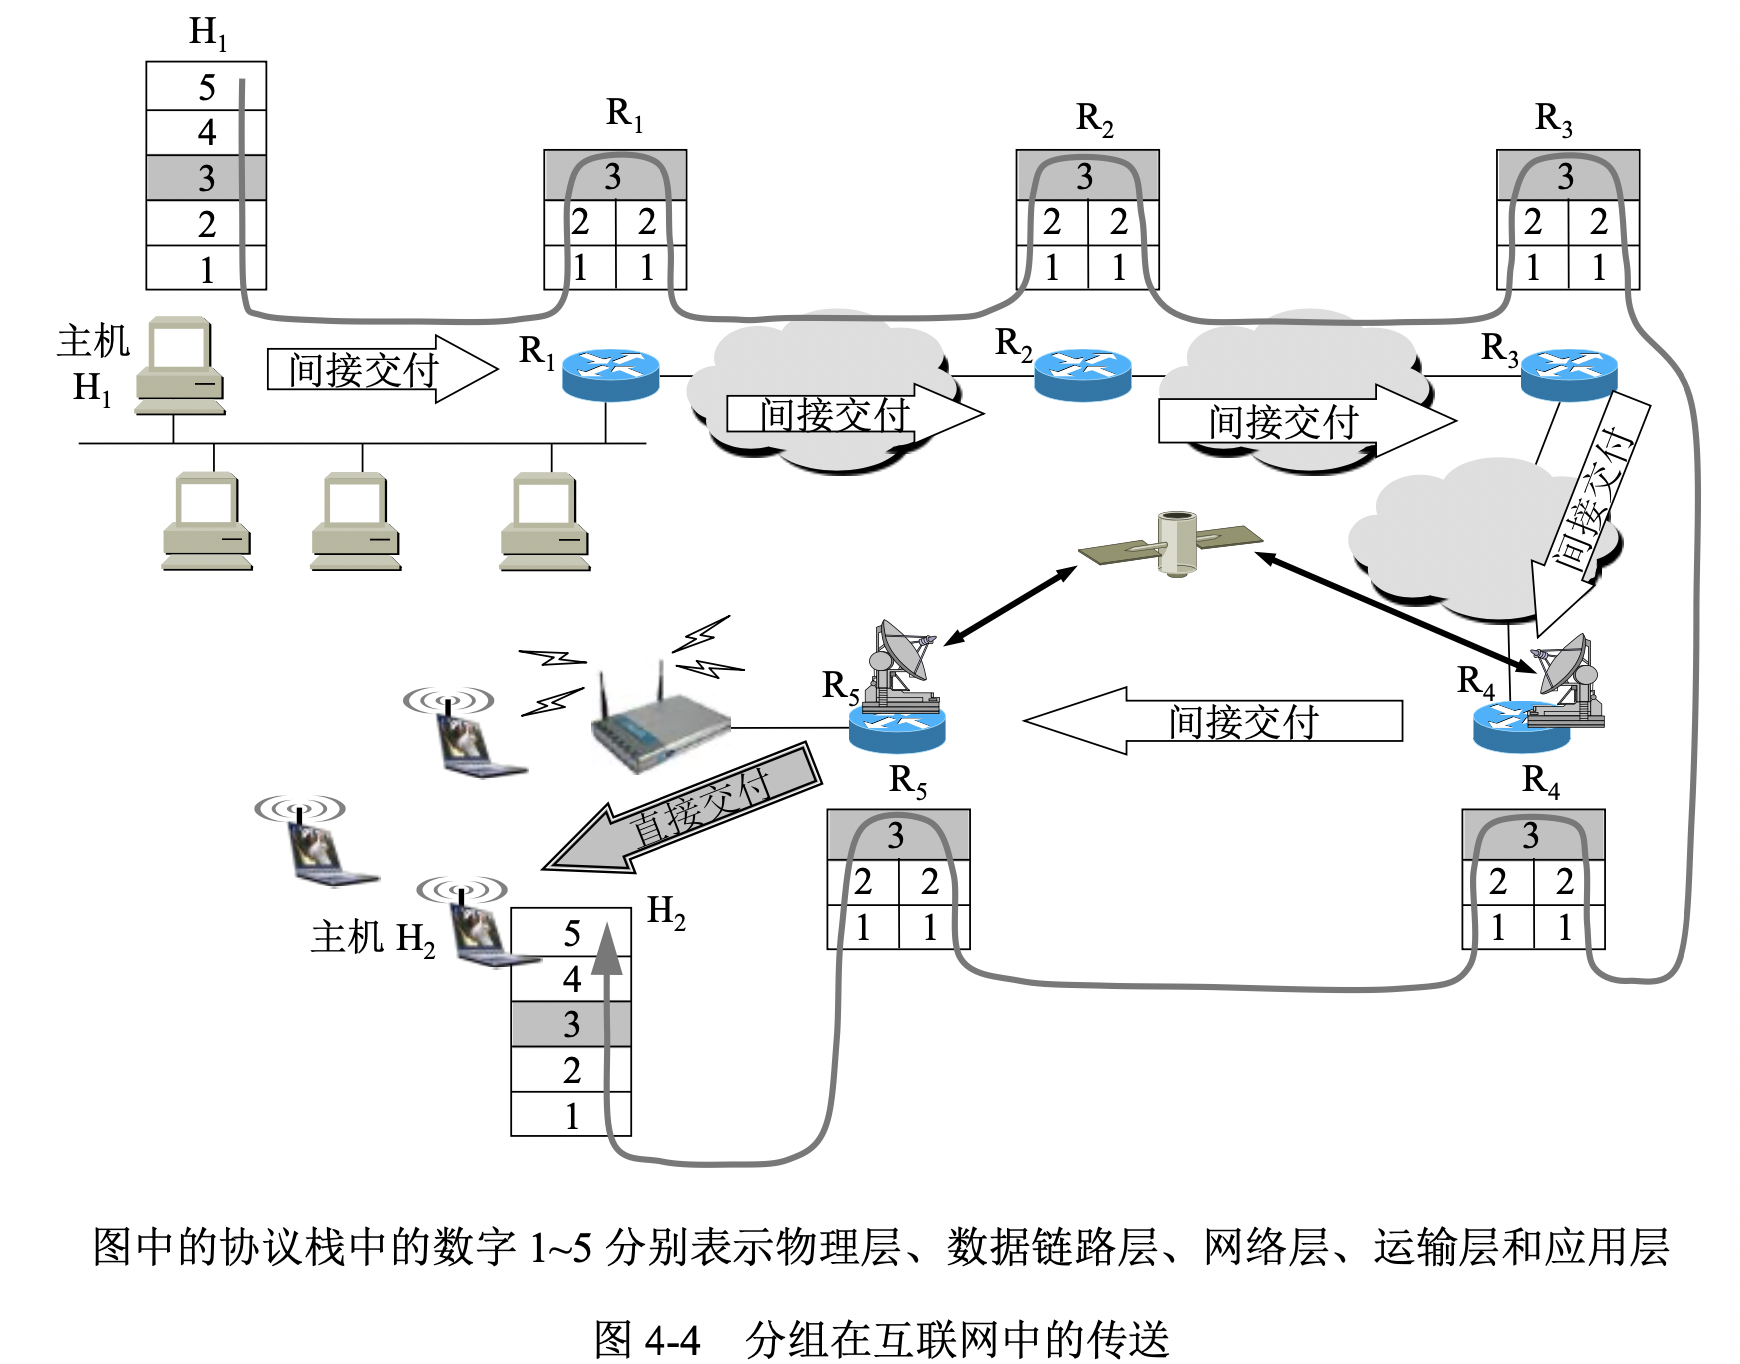
\includegraphics[width=0.7\textwidth]{img/4.4}
	\end{figure}

	\subsection{分类的IP地址}

	\subsubsection{IP地址及其表示方法}
	IP 地址的编址方法共经过了三个历史阶段
	\begin{itemize}
		\item 分类的 IP 地址。这是最基本的编址方法,在1981年就通过了相应的标准协议
		\item 子网的划分。这是对最基本的编址方法的改进,其标准 RFC950 在 1985 年通过
		\item 构成超网。这是比较新的无分类编址方法。1993年提出后很快就得到推广应用
	\end{itemize}

	本节只讨论最基本的分类的 IP 地址:
	
	所谓“分类的 IP 地址”就是将 IP 地址划分为若干个固定类,每一类地址都由两个固定长度的字段组成,其中第一个字段是网络号(net-id),它标志主机(或路由器)所连接到的网络。一个网络号在整个互联网范围内必须是唯一的。第二个字段是主机号(host-id),它标志该主机(或路由器)。这种两级的 IP 地址可以记为
	$$\mathrm{IP} \mbox{地址}\ ::=\ \{\mbox{<网络号>,<主机号>}\}$$

	\begin{figure}[H]
		\centering
		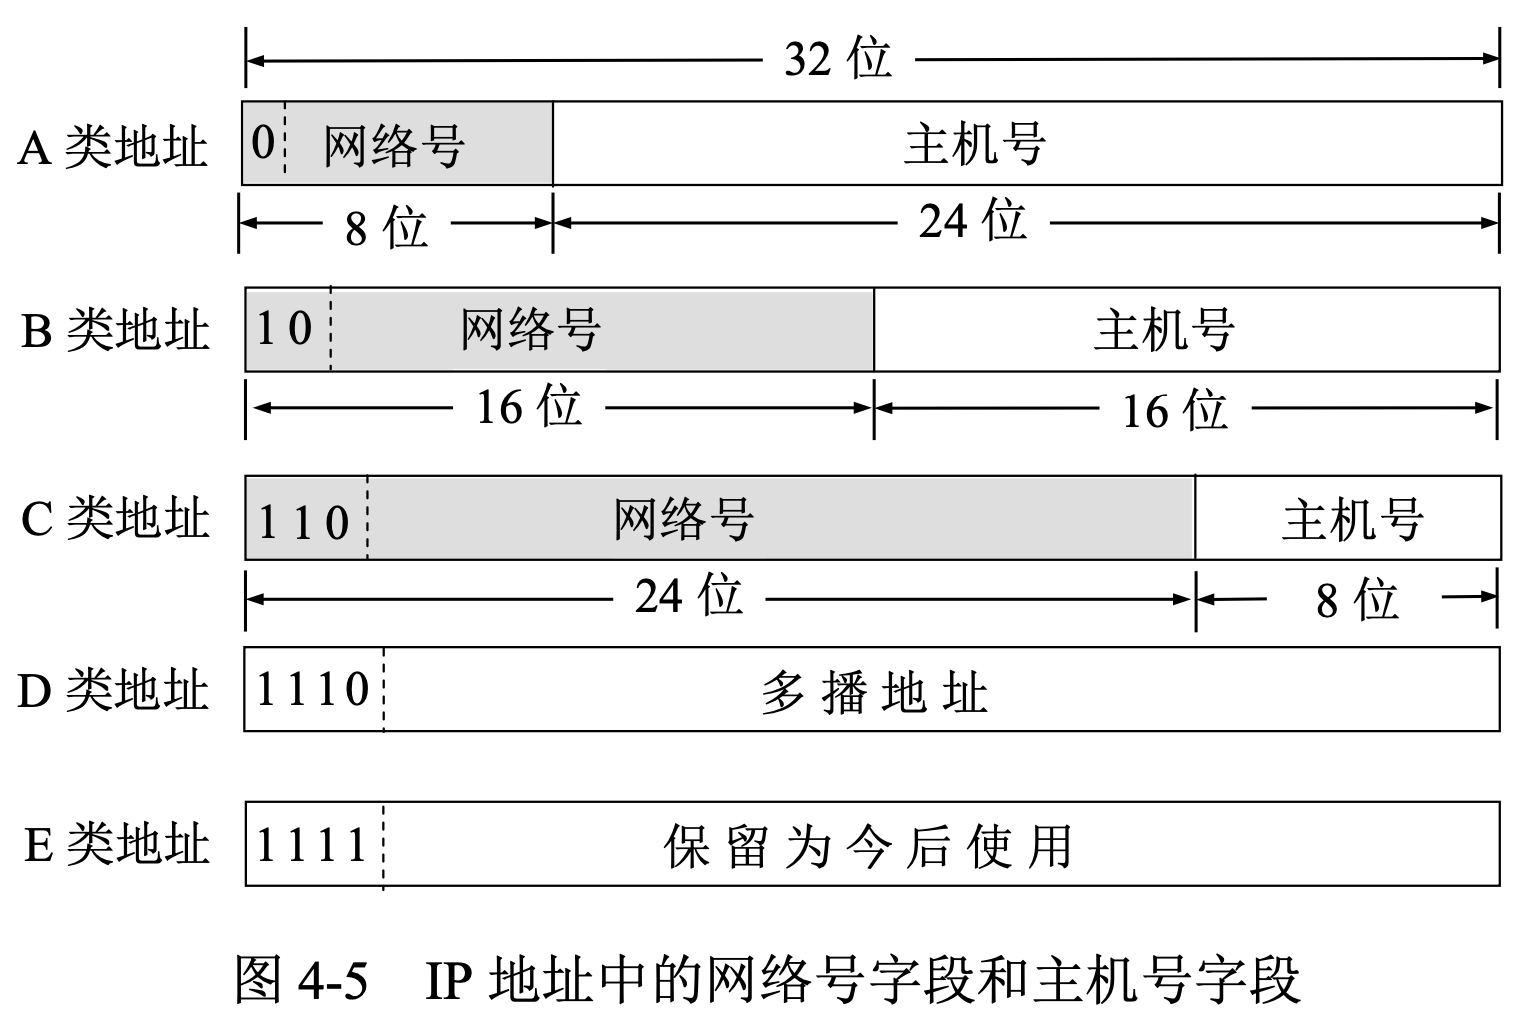
\includegraphics[width=0.6\textwidth]{img/4.5}
	\end{figure}
	\begin{itemize}
		\item A 类、B 类和 C 类地址的网络号字段分别为 1 个、2 个 和 3 个字节长,而在网络号字段的最前面有 1$\sim$3 位的类别位,其数值分别规定为 0,10和 110
		\item A 类、B 类和 C 类地址的主机号字段分别为 3 个、2 个和 1 个字节长
		\item D 类地址(前 4 位是 1110)用于多播
		\item E 类地址(前 4 位是 1111)保留为以后使用
		\item 只有 A 类、B 类和 C 类地址可以分配给网络中的主机或路由器的各接口
		\item 主机号为“全 0”的地址是网络地址,表示该 IP 地址是“本主机”所连接到的单个网络地址,不能分配给主机或路由器的各接口
		\item 主机号为“全 1”的地址是广播地址,表示该网络上的所有主机,不能分配给主机或路由器的各接口
	\end{itemize}

	\subsubsection{常用的三种类别的IP地址}
	\begin{figure}[H]
		\centering
		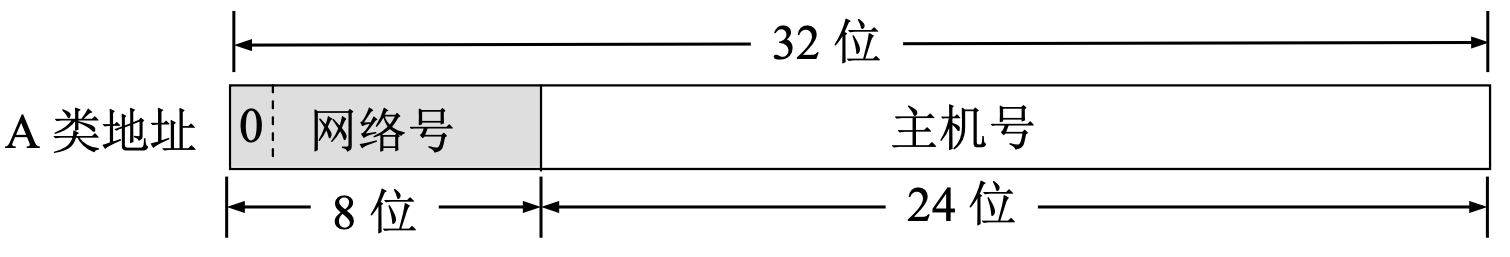
\includegraphics[width=0.65\textwidth]{img/4.2.2.1}
	\end{figure}
	 A 类地址的网络号字段占 1 个字节,只有 7 位可供使用(该字段的第一位已固定为0)
	\begin{itemize}
		\item 网络号字段为全 0(00000000)表示“本网络”,为保留字段,不指派
		\item 网络号为 127(01111111)保留作为本地软件环回测试本主机的进程之间的通信,不指派
		\begin{itemize}
			\item 最小的本地环回测试地址为 127.0.0.1
			\item 最大的本地环回测试地址为 127.255.255.254
		\end{itemize}
		\item 最后一个可指派的网络号为 126,网络地址为 126.0.0.0
		\item 可指派的网络数量为 $2^7 -2=126$
		\begin{itemize}
			\item 减 2 的原因是去掉最小网络号 0 和最大网络号 127
		\end{itemize}
		\item 每个网络中分配的 IP 地址数量为 $2^{24} - 2 = 16777214$
		\begin{itemize}
			\item 减 2 的原因是去掉主机号全 0 的网络地址和主机号全 1 的广播地址
		\end{itemize}
	\end{itemize}
	

	\begin{figure}[H]
		\centering
		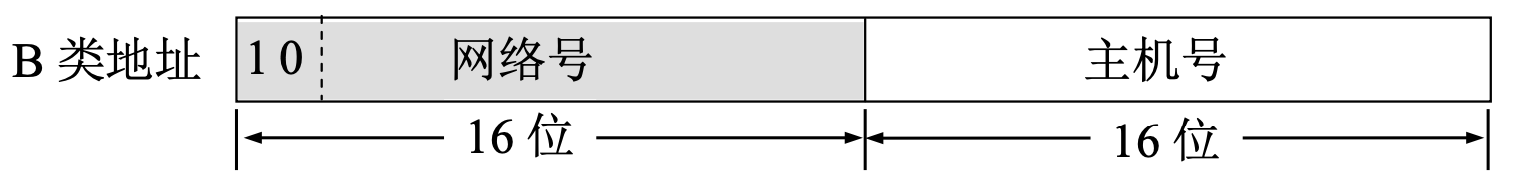
\includegraphics[width=0.65\textwidth]{img/4.2.2.2}
	\end{figure}
	B 类地址的网络号字段有 2 个字节,但前面两位(10)已经固定了,只剩下14位可以进行分配
	\begin{itemize}
		\item 最小网络号也是第一个可指派的网络号为 128.0,网络地址为 128.0.0.0
		\item 最大网络号也是最后一个可指派的网络号为 191.255,网络地址为 191.255.0.0
		\item 可指派的网络数量为 $2^{14} = 16384$
		\item 每个网络中分配的 IP 地址数量为 $2^{16} - 2 = 65534$
		\begin{itemize}
			\item 减 2 的原因是去掉主机号全 0 的网络地址和主机号全 1 的广播地址
		\end{itemize}
	\end{itemize}
		
	\begin{figure}[H]
		\centering
		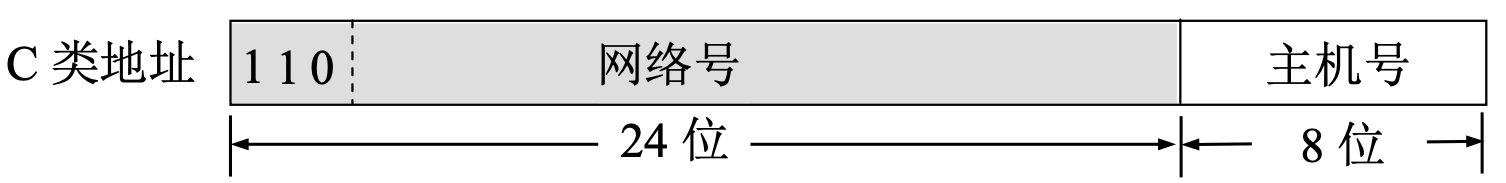
\includegraphics[width=0.65\textwidth]{img/4.2.2.3}
	\end{figure}
	C 类地址有 3 个字节的网络号字段,最前面的 3 位是(110),还有21位可以进行分配
	\begin{itemize}
		\item 最小网络号也是第一个可指派的网络号为 192.0.0,网络地址为 192.0.0.0
		\item 最大网络号也是最后一个可指派的网络号为 223.255.255,网络地址为 223.255.255.0
		\item 可指派的网络数量为 $2^{21} = 2097152$
		\item 每个网络中分配的 IP 地址数量为 $2^{8} - 2 = 254$
		\begin{itemize}
			\item 减 2 的原因是去掉主机号全 0 的网络地址和主机号全 1 的广播地址
		\end{itemize}
	\end{itemize}

	IP 地址的指派范围为
	\begin{table}[H]
		\centering
		\resizebox{\linewidth}{!}{
		\begin{tabular}{|c|c|c|c|c|}
		\hline
		网络类别 & 最大可指派的网络数         & 第一个可指派的网络号 & 最后一个可指派的网络号   & 每个网络中的最大主机数 \\ \hline
		A    & 126($2^7-2$)      & 1        & 126         & 16777214    \\ \hline
		B    & 16384($2^{14}$)   & 128.1    & 191.255     & 65534       \\ \hline
		C    & 2097152($2^{21}$) & 192.0.1  & 223.255.255 & 254         \\ \hline
		\end{tabular}
		}
	\end{table}

	一般不使用的特殊 IP 地址为
	\begin{table}[H]
		\centering
		\resizebox{\linewidth}{!}{
		\begin{tabular}{|c|c|c|c|c|}
		\hline
		网络号    & 主机号            & 源地址使用 & 目的地址使用 & 代表的意思                \\ \hline
		0      & 0              & 可以    & 不可     & 在本网络上的本主机            \\ \hline
		0      & host-id        & 可以    & 不可     & 在本网络上的某台主机 host-id   \\ \hline
		全 1    & 全 1            & 不可    & 可以     & 只在本网络上进行广播(各路由器均不转发) \\ \hline
		net-id & 全 1            & 不可    & 可以     & 对 net-id 上的所有主机进行广播  \\ \hline
		127    & 非全 0 或全 1 的任何数 & 可以    & 可以     & 用于本地软件环回测试           \\ \hline
		\end{tabular}
		}
	\end{table}

	IP 地址具有以下一些重要特点
	\begin{itemize}
		\item 每一个 IP 地址都由网络号和主机号两部分组成,IP 地址是一种分等级的地址结构
		\begin{itemize}
			\item IP 地址管理机构在分配 IP 地址时只分配网络号(第一级),而剩下的主机号(第二级)则由得到该网络号的单位自行分配。这样就方便了 IP 地址的管理
			\item 路由器仅根据目的主机所连接的网络号来转发分组(而不考虑目的主机号),这样就可以使路由表中的项目数大幅度减少,从而减小了路由表所占的存储空间以及查找路由表的时间
		\end{itemize}
		\item IP 地址是标志一台主机(或路由器)和一条链路的接口
		\item 一个网络是指具有相同网络号 net-id 的主机的集合,因此,用转发器或网桥连接起来的若干个局域网仍为一个网络
		\item 在 IP 地址中,所有分配到网络号的网络都是平等的。所谓平等,是指互联网同等对待每一个 IP 地址
	\end{itemize}

	\begin{figure}[H]
		\centering
		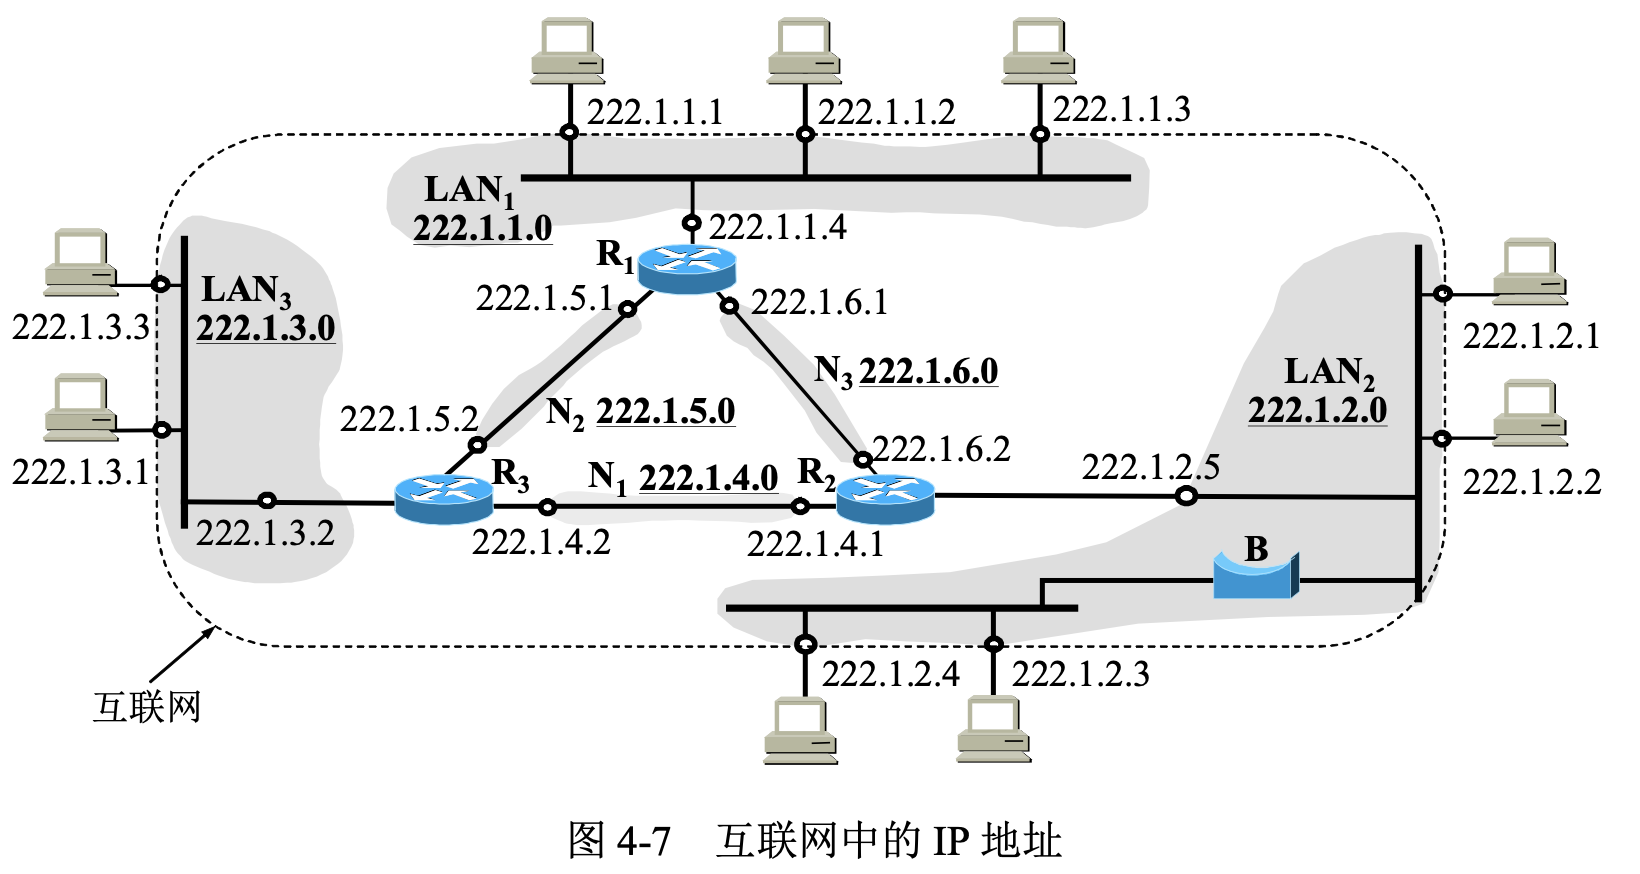
\includegraphics[width=0.75\textwidth]{img/4.7}
	\end{figure}

	\subsection{IP地址与硬件地址}
	\begin{figure}[H]
		\centering
		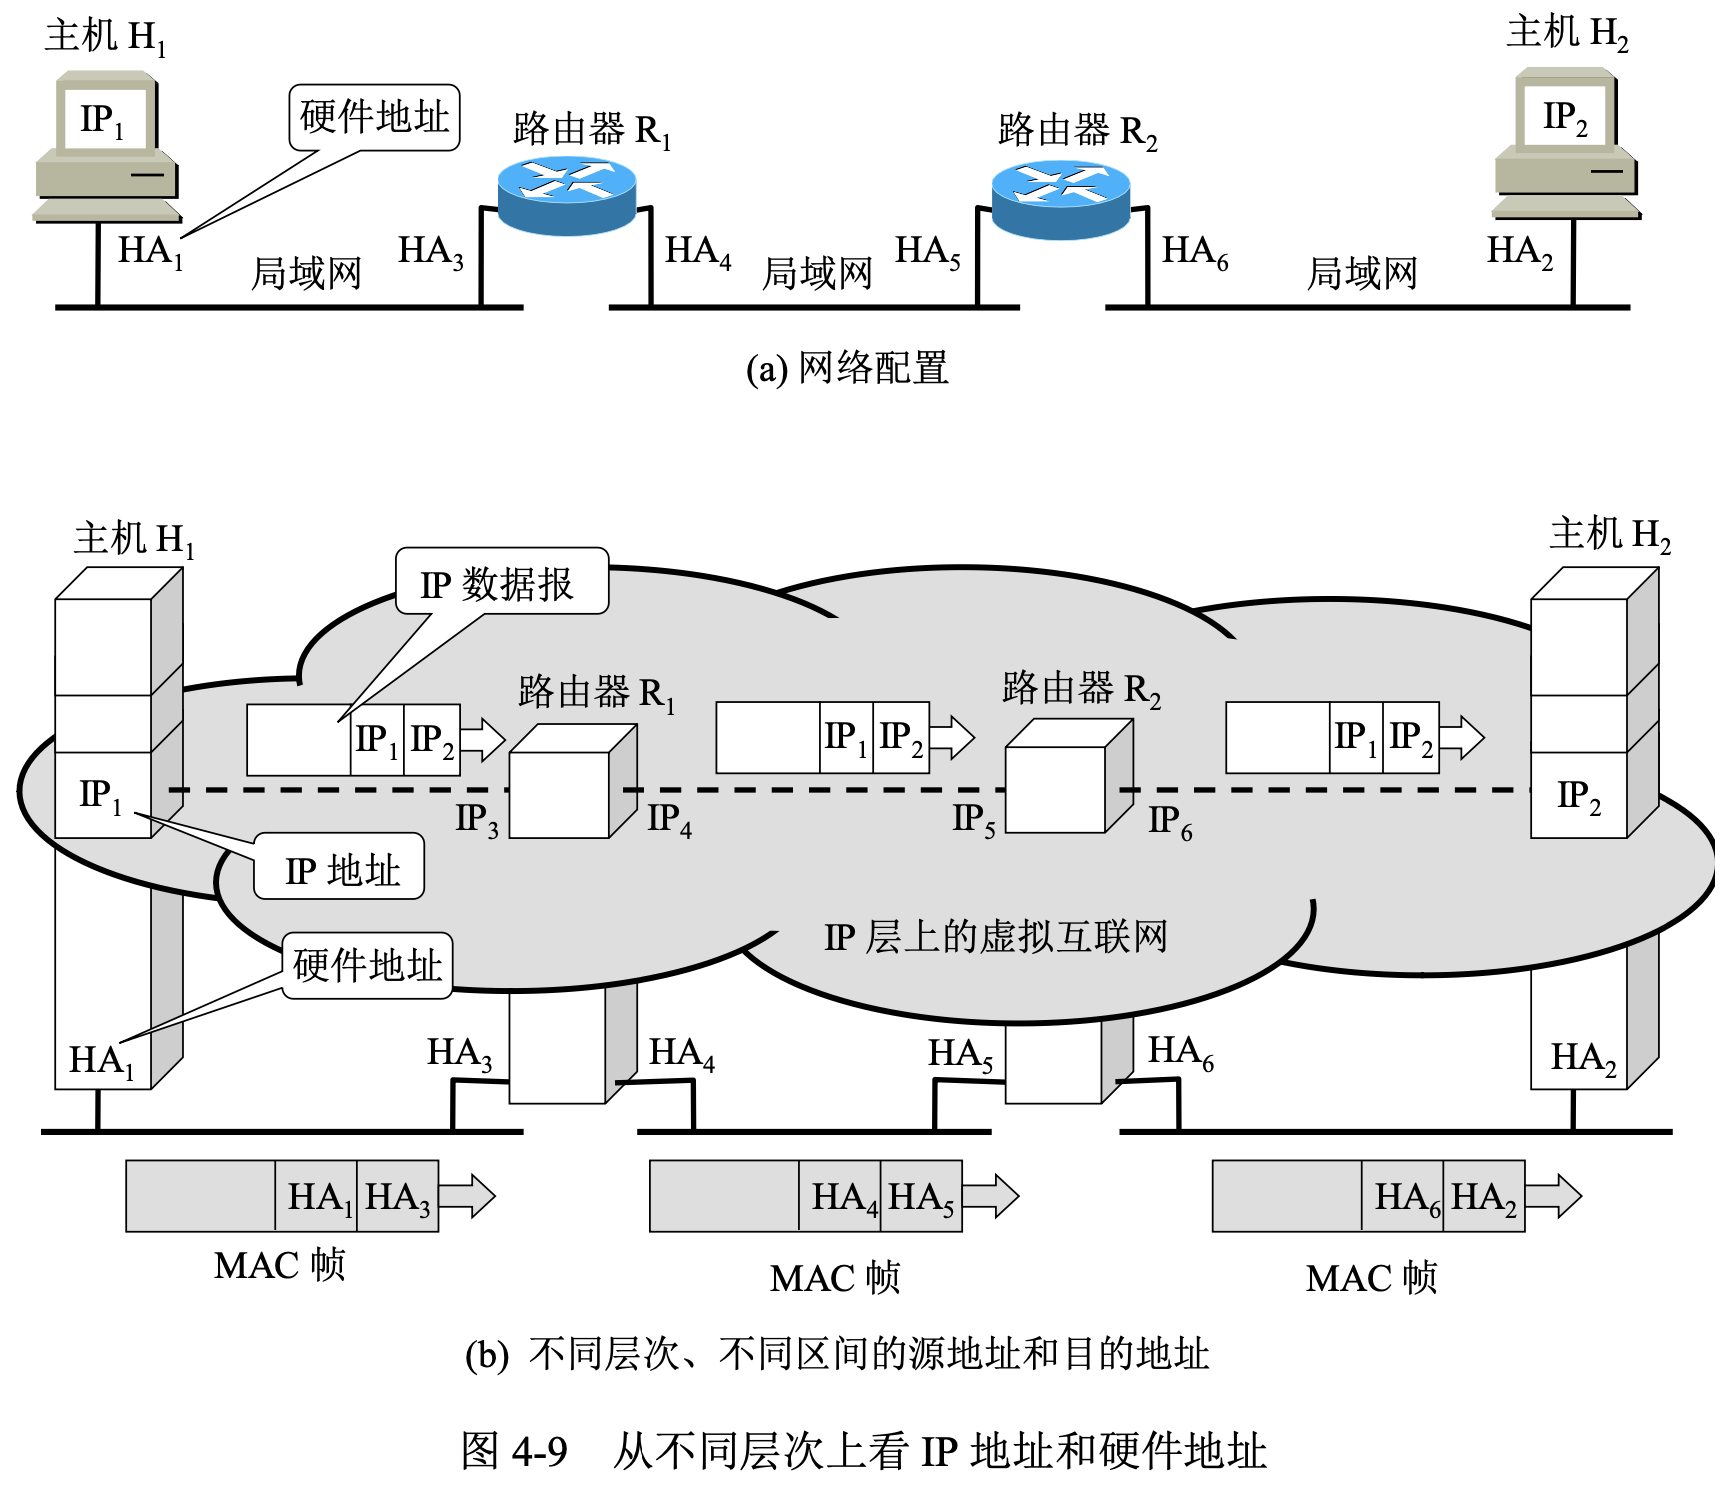
\includegraphics[width=0.85\textwidth]{img/4.9}
	\end{figure}

	\begin{itemize}
		\item 数据包转发过程中源 IP 地址和目的 IP 地址保持不变
		\item 数据包转发过程中源 MAC 地址和目的 MAC 地址逐个链路(或逐个网络)改变
	\end{itemize}

	\subsection{地址解析协议ARP}

	\begin{itemize}
		\item 地址解析协议 ARP 用来解决已经知道一个机器(主机或路由器)的 IP 地址,需要找出其相应的硬件地址的问题
		\item 地址解析协议 ARP 解决这个问题的方法是在主机 ARP 高速缓存中存放一个从 IP 地址到硬件地址的映射表,并且这个映射表还经常动态更新(新增或超时删除)
		\item 每一台主机都设有一个 ARP 高速缓存(ARP cache),里面有本局域网上的各主机和路由器的 IP 地址到硬件地址的映射表
	\end{itemize}

	ARP 映射表的构造过程如下:
	\begin{figure}[H]
		\centering
		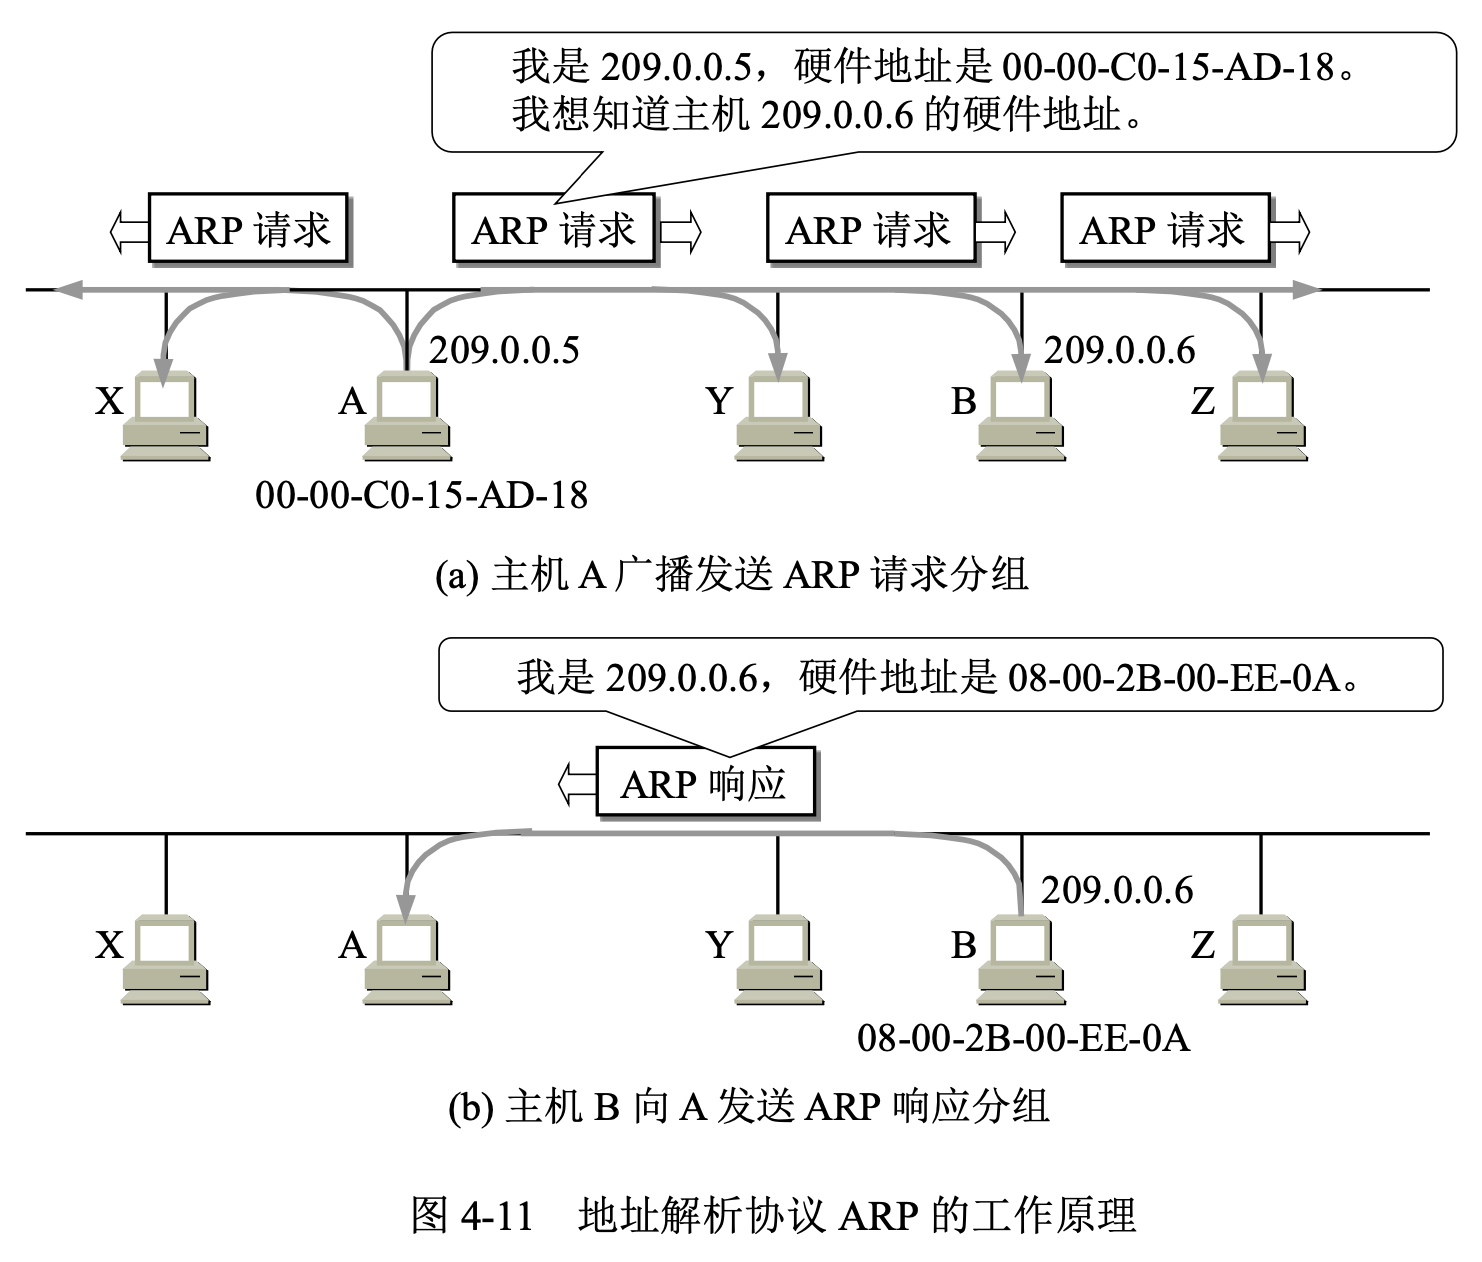
\includegraphics[width=0.65\textwidth]{img/4.11}
	\end{figure}
	\begin{itemize}
		\item 当主机 A 要向本局域网上的某台主机 B 发送 IP 数据报时,就先在其 ARP 高速缓存中查看有无主机 B 的 IP 地址。如有,就在 ARP 高速缓存中查出其对应的硬件地址,再把这个硬件地址写入 MAC 帧,然后通过局域网把该 MAC 帧发往此硬件地址
		\item 也有可能查不到主机 B 的 IP 地址的项目。这可能是主机 B 才入网,也可能是主机 A 刚刚加电,其高速缓存还是空的。在这种情况下,主机 A 就自动运行 ARP,然后按以下步骤找出主机 B 的硬件地址:
		\begin{itemize}
			\item ARP 进程在本局域网上广播发送一个ARP 请求分组,其主要内容是:“我的 IP 地址是 209.0.0.5,硬件地址是 00-00-C0-15-AD-18。我想知道 IP 地址为 209.0.0.6 的主机的硬件地址。”
			\item 在本局域网上的所有主机上运行的 ARP 进程都收到此 ARP 请求分组
			\item 主机 B 的 IP 地址与 ARP 请求分组中要查询的 IP 地址一致,就收下这个 ARP 请求分组,并向主机 A 发送 ARP 响应分组(单播),其主要内容是:“我的 IP 地址是 209.0.0.6,我的硬件地址是 08-00-2B-00-EE-0A。”,同时将主机 A 的地址映射关系写入自己的 ARP 高速缓存中。其余的所有主机的 IP 地址都与 ARP 请求分组中要查询的 IP 地址不一致,因此都不理睬这个 ARP 请求分组
			\item 主机 A 收到主机 B 的 ARP 响应分组后,就在其 ARP 高速缓存中写入主机 B 的 IP 地址到硬件地址的映射
		\end{itemize}
		\item ARP 对保存在高速缓存中的每一个映射地址项目都设置生存时间,凡超过生存时间的项目就从高速缓存中删除掉
	\end{itemize}

	使用 ARP 的四种典型情况:
	\begin{figure}[H]
		\centering
		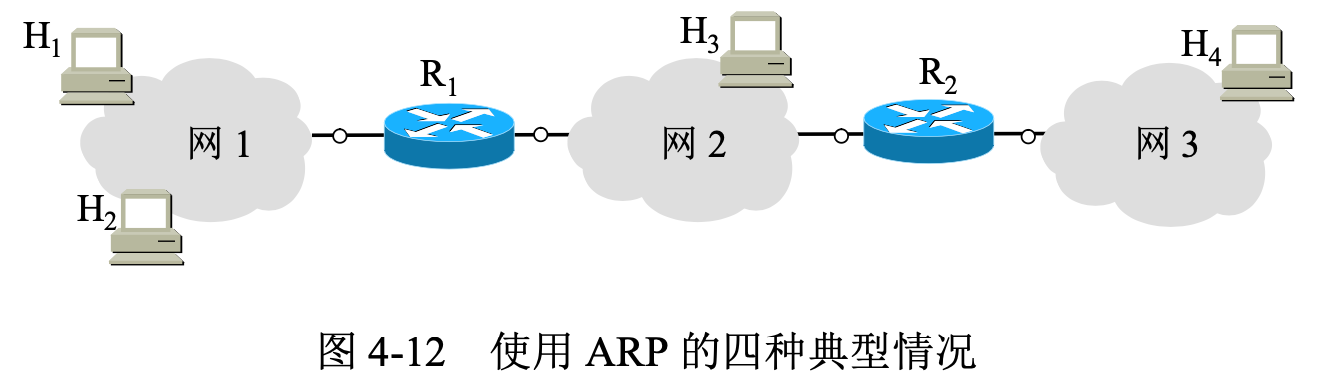
\includegraphics[width=0.75\textwidth]{img/4.12}
	\end{figure}
	\begin{enumerate}[label=\arabic*.]
		\item 发送方是主机(如 $H_1$),要把 IP 数据报发送到同一个网络上的另一台主机(如 $H_2$)。这时 $H_1$ 发送 ARP 请求分组(在网 1 上广播),找到目的主机 $H_2$ 的硬件地址
		\item 发送方是主机(如 $H_1$),要把 IP 数据报发送到另一个网络上的一台主机(如 $H_3$ 或 $H_4$)。这时 $H_1$ 发送 ARP 请求分组(在网 1 上广播),找到网 1 上的一个路由器 $R_1$ 的硬件地址。剩下的工作由路由器 $R_1$ 来完成。$R_1$ 要做的事情是下面的3或4
		\item 发送方是路由器(如 $R_1$),要把 IP 数据报转发到与 $R_1$ 连接在同一个网络(网 2)上的主机(如 $H_3$)。这时 $R_1$ 发送 ARP 请求分组(在网 2 上广播),找到目的主机 $H_3$ 的硬件地址
		\item 发送方是路由器(如 $R_1$),要把 IP 数据报转发到网 3 上的一台主机(如 $H_4$)。$H_4$ 与 $R_1$ 不是连接在同一个网络上。这时 $R_1$ 发送 ARP 请求分组(在网 2 上广播),找到连接在网 2 上的一个路由器 $R_2$ 的硬件地址。剩下的工作由这个路由器 $R_2$ 来完成
	\end{enumerate}

	\subsection{IP数据报的格式}
	\begin{figure}[H]
		\centering
		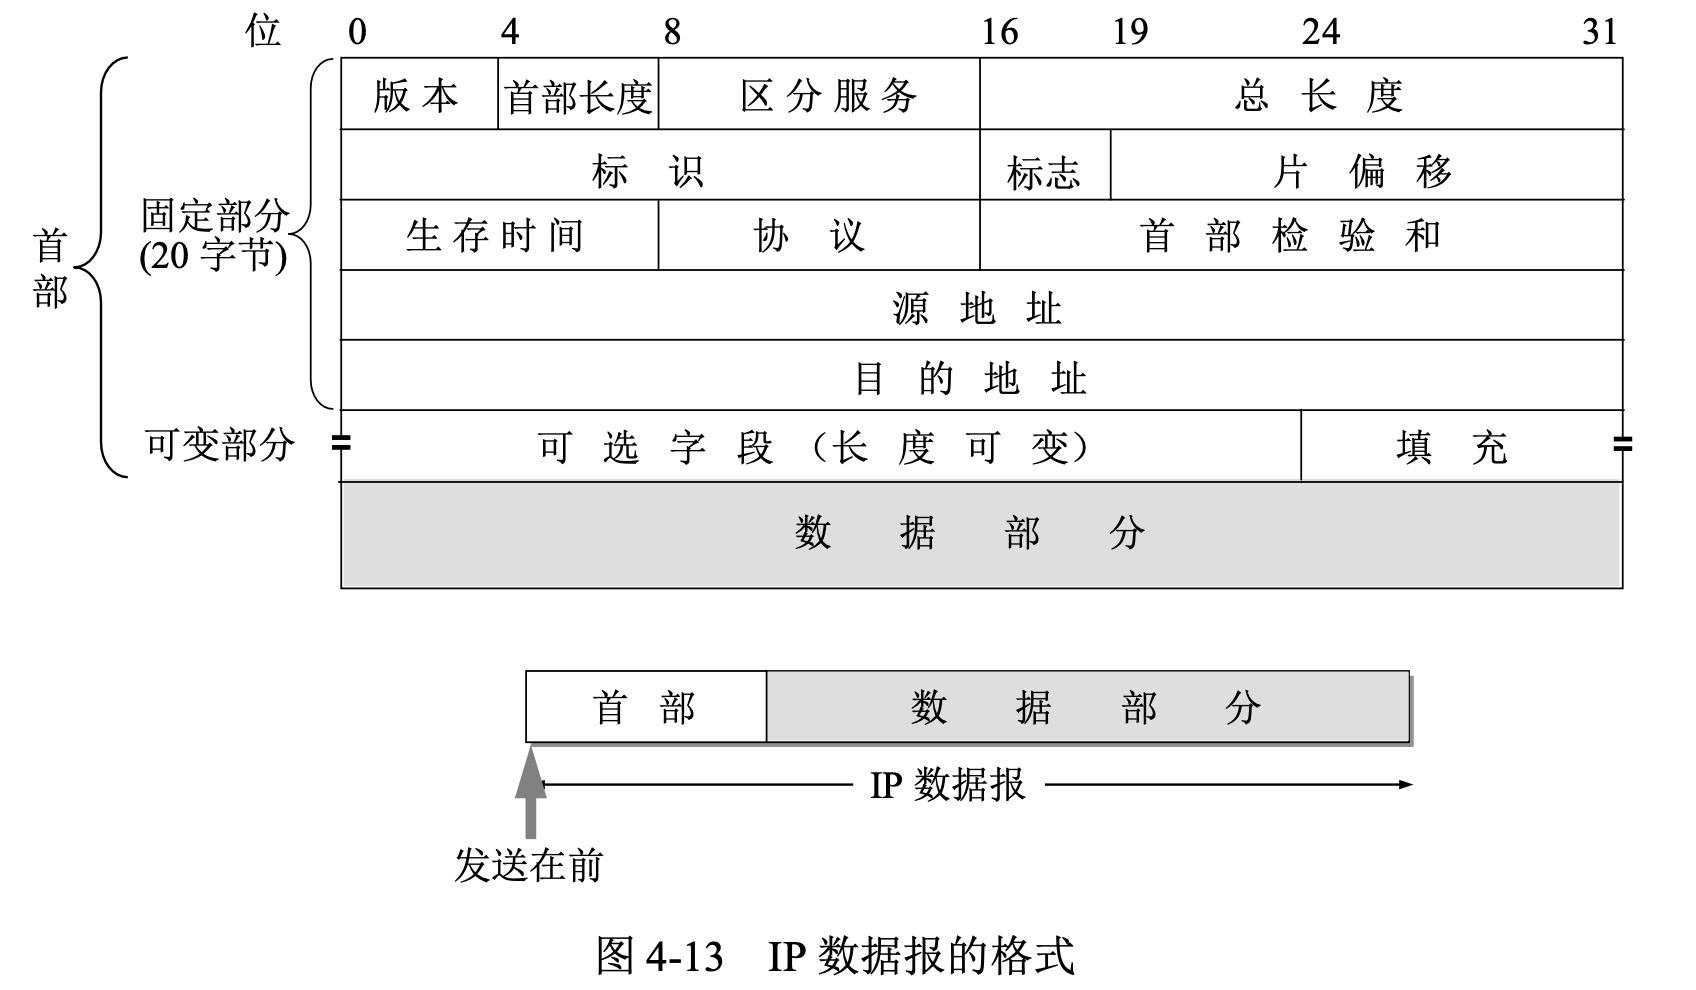
\includegraphics[width=0.6\textwidth]{img/4.13}
	\end{figure}

	\subsubsection{IP数据报首部的固定部分中的各字段}

	\paragraph{版本}~{}

	占 4 比特,表示 IP 协议的版本,通信双方使用的 IP 协议的版本必须一致,目前广泛使用的 IP 协议版本号为4(即 IPv4)

	\paragraph{首部长度}~{}

	占 4 比特,表示 IP 数据报首部的长度,该字段所表示数的单位是 32 位字(即 4 字节)
	\begin{itemize}
		\item 最小十进制取值为 5,表示 IP 数据报首部只有 20 字节固定部分
		\item 最大十进制取值为 15,表示 IP 数据报首部包含 20 字节固定部分和最大 40 字节的可变部分
	\end{itemize}

	\paragraph{区分服务}~{}

	\begin{itemize}
		\item 占 8 比特,用来获得更好的服务
		\item 这个字段在旧标准中叫做服务类型, 但实际上一直没有被使用过。1998 年 IETF 把这个字段改名为区分服务 DS(Differentiated Services)
		\item 只有在使用区分服务时,这个字段才起作用。在一般的情况下都不使用这个字段
	\end{itemize}

	\paragraph{总长度}~{}

	占 16 比特,表示 IP 数据报的总长度,即 IP 数据报首部长度和数据载荷长度之和

	\paragraph{标识(identification)}~{}

	占 16 比特,属于同一个数据报的各分片数据报应该具有相同的标识。IP 软件维持一个计数器,每产生一个数据报,计数器值加 1 ,并将此值赋值给标识字段

	\paragraph{标志(flag)}~{}

	占 3 比特,但目前只有两位有意义
	\begin{itemize}
		\item 标志字段中的最低位记为MF(More Fragment)。$\mathrm{MF}=1$ 即表示后面“还有分片” 的数据报。$\mathrm{MF}=0$ 表示这已是若干数据报片中的最后一个
		\item 标志字段中间的一位记为 DF(Don’t Fragment),意思是“不能分片”。只有当 $\mathrm{DF}=0$ 时才允许分片
	\end{itemize}

	\paragraph{片偏移}~{}

	占 13 位。片偏移指出:较长的分组在分片后,某片在原分组中的相对位置。也就是说,相对于用户数据字段的起点,该片从何处开始。片偏移以 8 个字节为偏移单位。这就是说,每个分片的长度一定是 8 字节(64 位)的整数倍

	\textbf{例:}对 IPv4 数据报进行分片

	一数据报的总长度为 3820 字节,其数据部分为 3800 字节长(使用固定首部),需要分片为长度不超过 1420 字节的数据报片
	\begin{figure}[H]
		\centering
		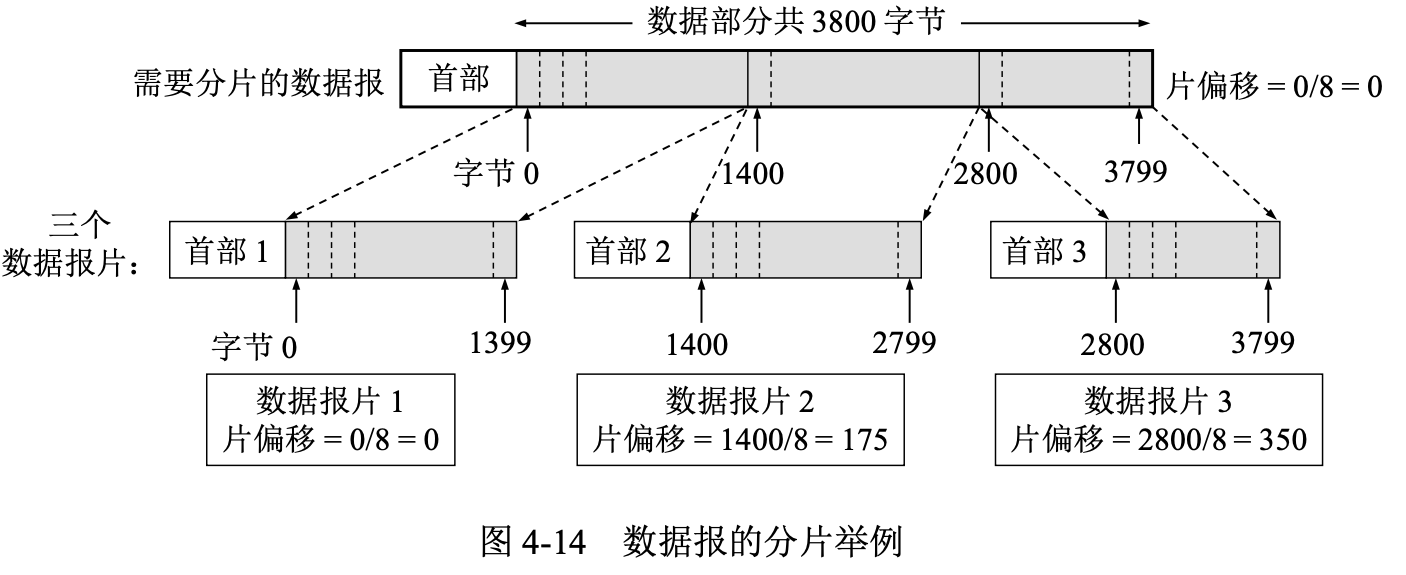
\includegraphics[width=0.8\textwidth]{img/4.14}
	\end{figure}

	\begin{table}[H]
		\centering
		\begin{tabular}{|c|c|c|c|c|c|}
		\hline
		\textbf{} & 总长度  & 标识    & MF & DF & 片偏移 \\ \hline
		原始数据报     & 3820 & 12345 & 0  & 0  & 0   \\ \hline
		数据报片1     & 1420 & 12345 & 1  & 0  & 0   \\ \hline
		数据报片2     & 1420 & 12345 & 1  & 0  & 175 \\ \hline
		数据报片3     & 1020 & 12345 & 0  & 0  & 350 \\ \hline
		\end{tabular}
	\end{table}

	现假定数据报片2经过某个网络时还需要再进行分片,即划分为数据报片2-1(携带数据800字节)和数据报片2-2(携带数据600字节)

	\begin{table}[H]
		\centering
		\begin{tabular}{|c|c|c|c|c|c|}
		\hline
		\textbf{} & 总长度  & 标识    & MF & DF & 片偏移 \\ \hline
		原始数据报     & 3820 & 12345 & 0  & 0  & 0   \\ \hline
		数据报片2-1   & 820  & 12345 & 1  & 0  & 175 \\ \hline
		数据报片2-2   & 620  & 12345 & 1  & 0  & 275 \\ \hline
		数据报片3     & 1020 & 12345 & 0  & 0  & 350 \\ \hline
		\end{tabular}
	\end{table}

	\paragraph{生存时间TTL}~{}

	\begin{itemize}
		\item 占 8 比特。最初以秒为单位,最大生存周期为 255 秒。路由器转发 IP 数据报时,将 IP 数据报首部中的该字段的值减去 IP 数据报在本路由器上所耗费的时间,若不为 0 则转发,否则就丢弃
		\item 现在以“跳数”为单位,路由器转发 IP 数据报时,将 IP 数据报首部中的该字段的值减 1,若不为 0 就转发,否则就丢弃
	\end{itemize}

	\paragraph{协议}~{}

	占 8 比特,协议字段指出此数据报携带的数据是使用何种协议,以便使目的主机的 IP 层知道应将数据部分上交给哪个协议进行处理

	\paragraph{首部检验和}~{}

	\begin{itemize}
		\item 占 16 比特,用来检验首部在传输过程中是否有差错。比 CRC 校验码简单,称为因特网检验和
		\item IP 数据报每经过一个路由器,路由器都要重新计算一下首部检验和,这是因为某些字段(生存时间、标志、片偏移等)的取值可能发生会发生变化
		\item 由于 IP 层本身并不提供可靠传输服务,且计算首部检验和是一项耗时的操作,因此在 IPv6 中,路由器不再计算首部检验和,从而更快转发 IP 数据报
	\end{itemize}
	\begin{figure}[H]
		\centering
		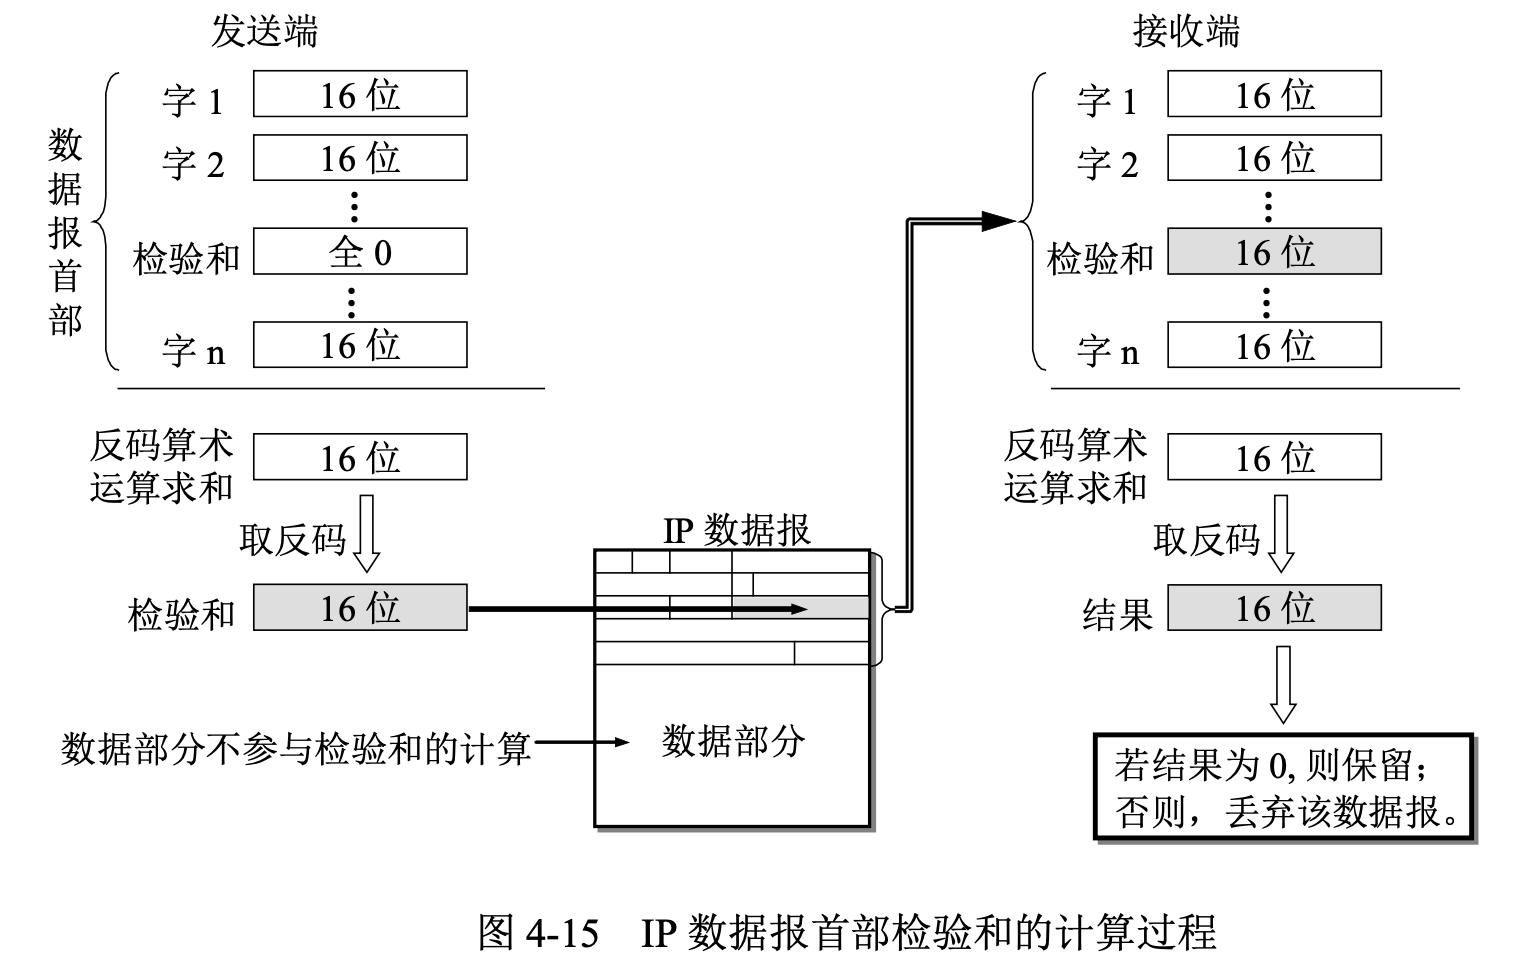
\includegraphics[width=0.6\textwidth]{img/4.15}
	\end{figure}

	\paragraph{源地址}~{}

	占 32 比特

	\paragraph{目的地址}~{}
	
	占 32 比特

	\subsubsection{IP数据报首部的可变部分}
	\begin{itemize}
		\item IP 数据报首部的可变部分就是一个选项字段。选项字段用来支持排错、测量以及安全等措施
		\item 此字段的长度可变,从 1 个字节到 40 个字节不等,取决于所选择的项目
		\item 增加首部的可变部分是为了增加 IP 数据报的功能,但这同时也使得 IP 数据报的首部长 度成为可变的。这就增加了每一个路由器处理数据报的开销。实际上这些选项很少被使用
		\item 为了确保首部长度为 4 字节的整数倍,有时需要用全 0 的填充字段将其补齐
	\end{itemize}


	\subsection{IP层转发分组的流程}
	\begin{figure}[H]
		\centering
		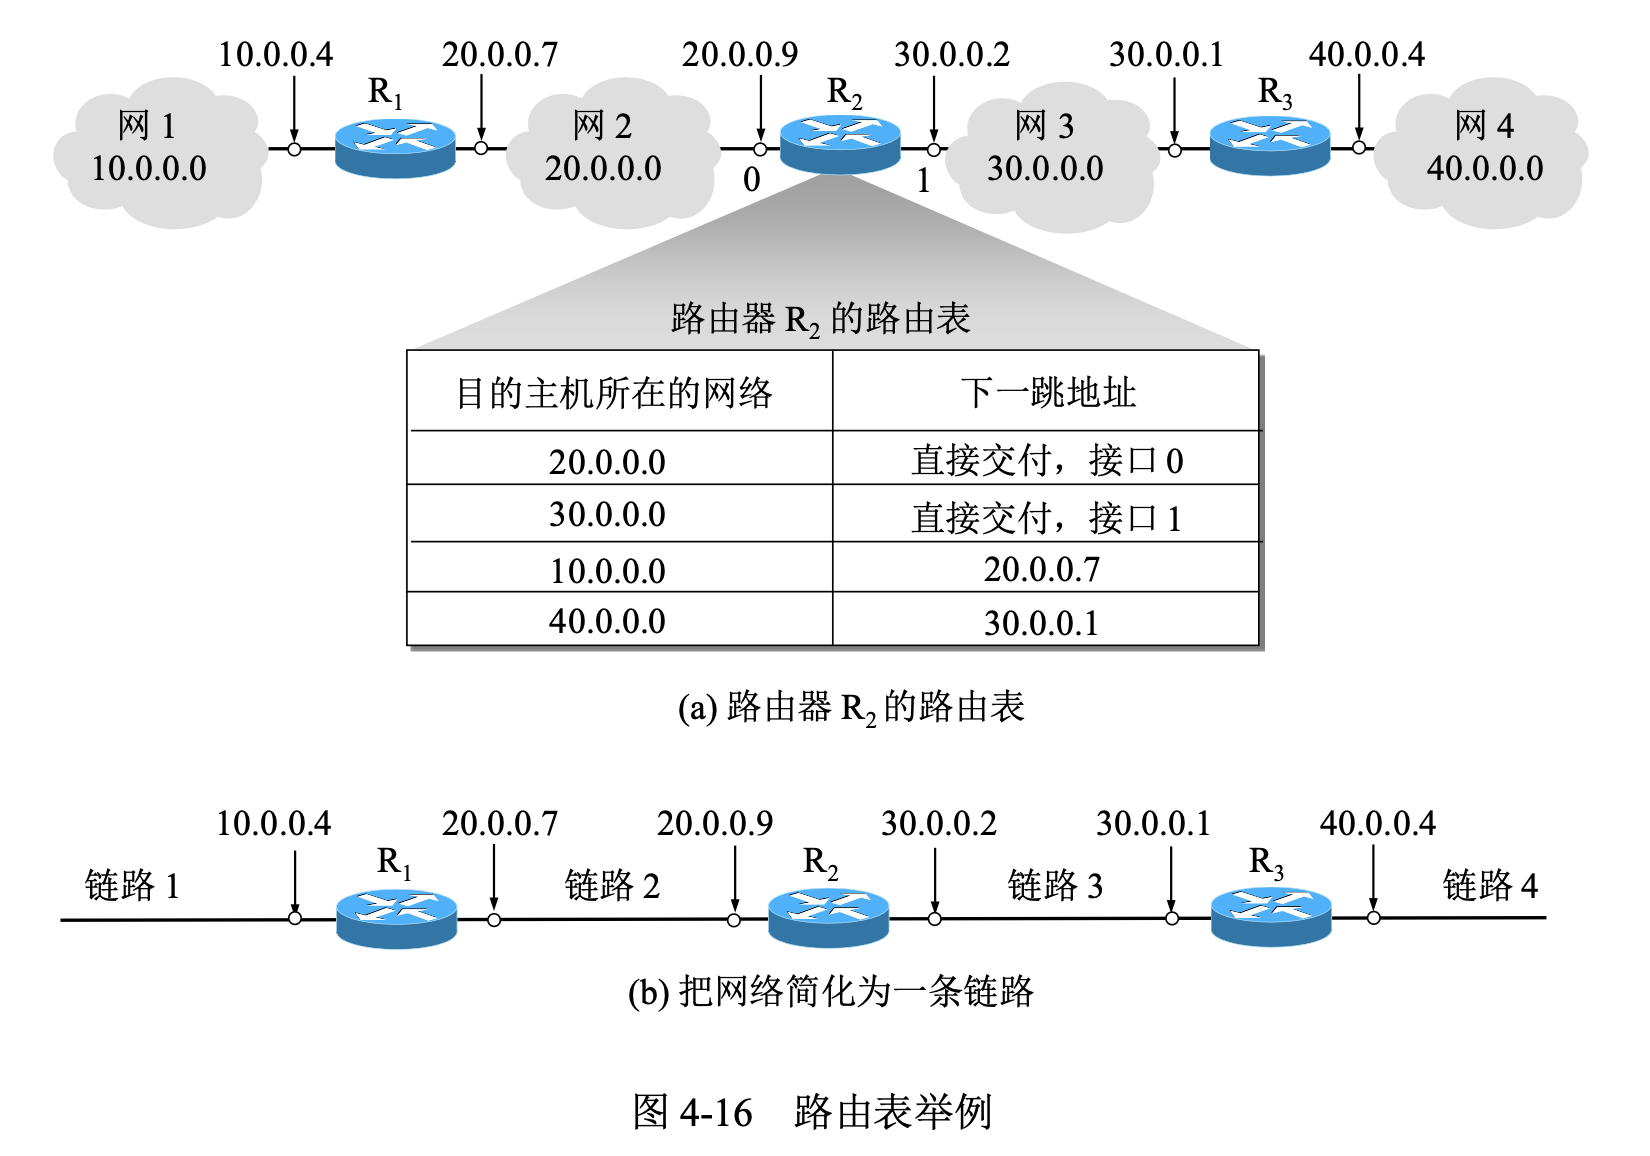
\includegraphics[width=0.7\textwidth]{img/4.16}
	\end{figure}

	分组转发算法如下:
	\begin{enumerate}[label=\arabic*.]
		\item 从数据报的首部提取目的主机的 IP 地址 $D$, 得出目的网络地址为 $N$
		\item 若 $N$ 就是与此路由器直接相连的某个网络地址,则进行直接交付,不需要再经过其他的路由器,直接把数据报交付目的主机(这里包括把目的主机地址 $D$ 转换为具体的硬件地址,把数据报封装为 MAC 帧,再发送此帧);否则就是间接交付,执行 3
		\item 若路由表中有目的地址为 $D$ 的特定主机路由,则把数据报传送给路由表中所指明的下一跳路由器;否则,执行 4
		\item 若路由表中有到达网络 $N$ 的路由,则把数据报传送给路由表中所指明的下一跳路由器;否则,执行 5
		\item 若路由表中有一个默认路由,则把数据报传送给路由表中所指明的默认路由器;否则,执行 6
		\item 报告转发分组出错
	\end{enumerate}

	\section{划分子网和构造超网}

	\subsection{划分子网}

	\subsubsection{从两级 IP 地址到三级 IP 地址}

	划分子网的基本思路为:
	\begin{itemize}
		\item 一个拥有许多物理网络的单位,可将所属的物理网络划分为若干个子网。划分子网纯属一个单位内部的事情。本单位以外的网络看不见这个网络是由多少个子网组成, 因为这个单位对外仍然表现为一个网络
		\item 划分子网的方法是从网络的主机号借用若干位作为子网号,于是两级 IP 地址在本单位内部就变为三级 IP 地址:网络号、 子网号和主机号。也可以用以下记法来表示:$${\mathrm{IP}} \mbox{地址}\ ::=\ \{\mbox{<网络号>,<子网号>,主机号<>}\}$$
		\item 凡是从其他网络发送给本单位某台主机的 IP 数据报,仍然是根据 IP 数据报的目的 网络号找到连接在本单位网络上的路由器。但此路由器在收到 IP 数据报后,再按目的网络 号和子网号找到目的子网,把 IP 数据报交付目的主机
	\end{itemize}

	\subsubsection{子网掩码}
	32 比特的子网掩码可以表明分类 IP 地址的主机号部分被借用了几个比特作为子网号
	\begin{itemize}
		\item 子网掩码使用连续的比特1来对应网络号和子网号
		\item 子网掩码使用连续的比特0来对应主机号
		\item 将划分子网的IPv4地址与其相应的子网掩码进行逻辑与运算就可得到IPv4地址所在子网的网络地址
	\end{itemize}
	\begin{figure}[H]
		\centering
		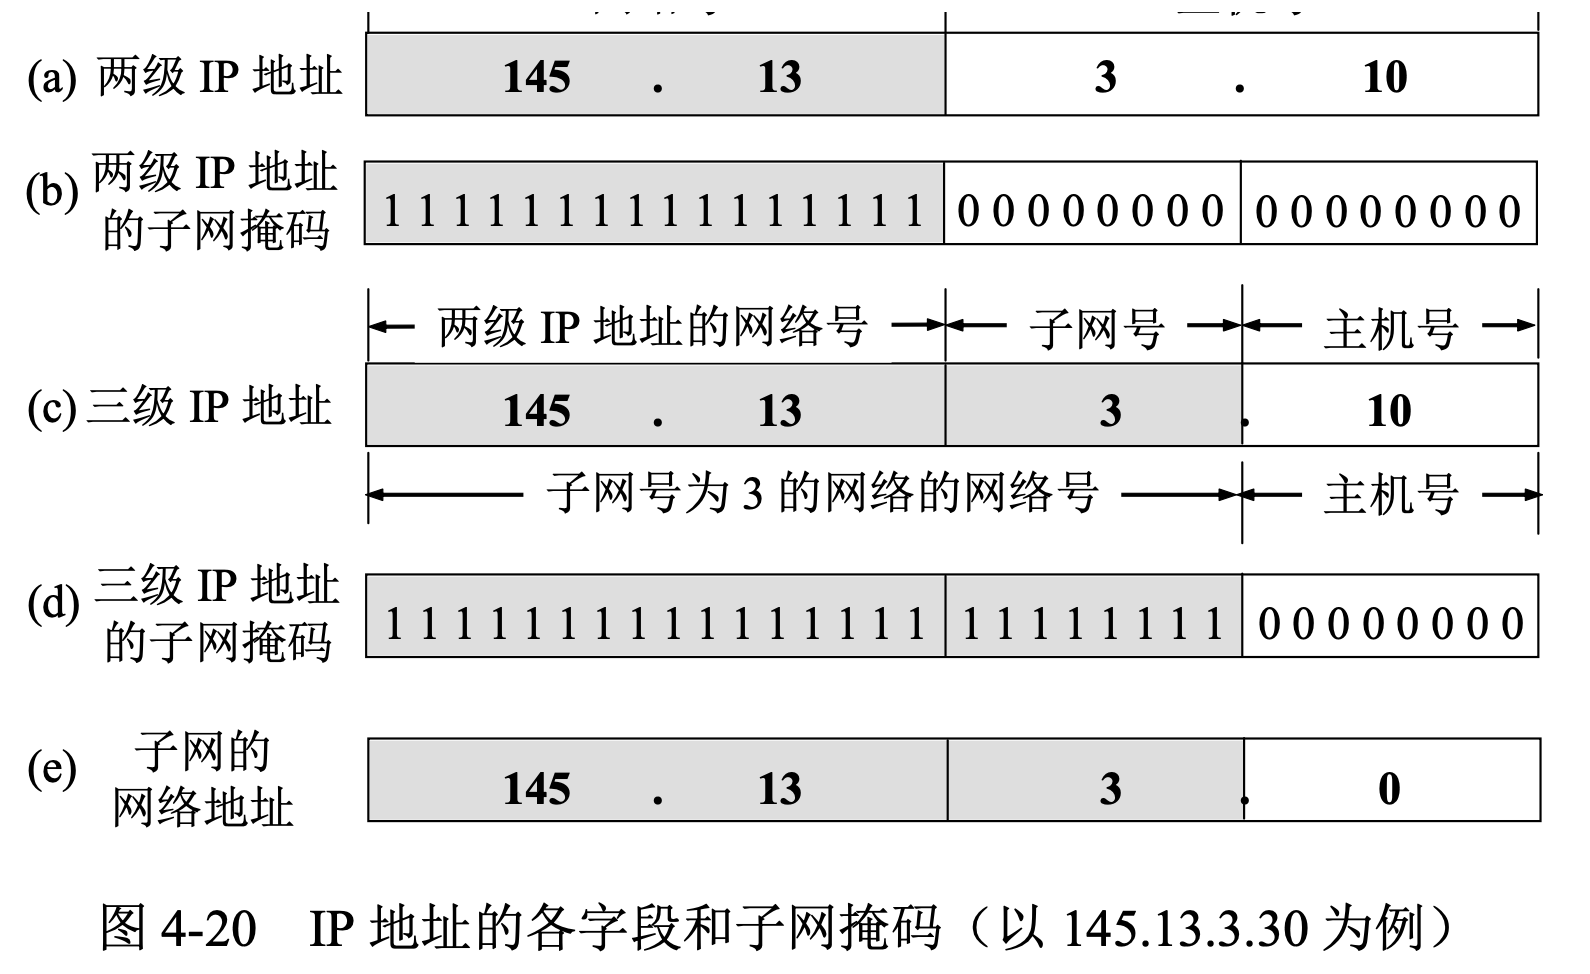
\includegraphics[width=0.7\textwidth]{img/4.20}
	\end{figure}

	默认的子网掩码是指在未划分子网的情况下使用的子网掩码
	\begin{figure}[H]
		\centering
		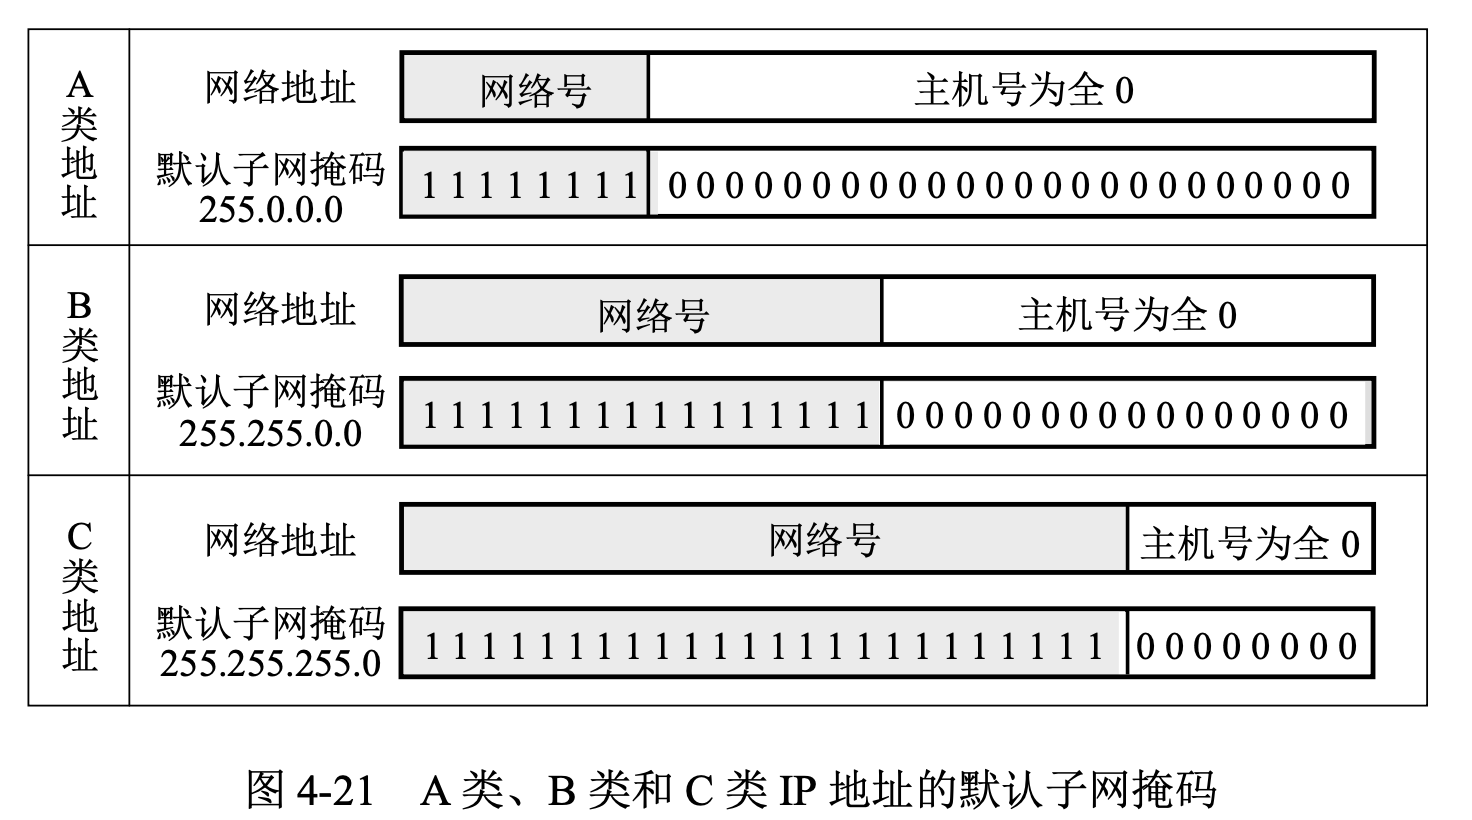
\includegraphics[width=0.7\textwidth]{img/4.21}
	\end{figure}

	\textbf{例:}已知某个网络的地址为 218.75.230.0,使用子网掩码 255.255.255.128 对其进行子网划分,请给出划分细节
	\begin{table}[H]
		\centering
		\begin{tabular}{|c|c|c|c|}
		\hline
		网络号        & 子网号 & 主机号      & 具体含义                    \\ \hline
		218.75.230 & 0   & 000 0000 & 子网0的网络地址 218.75.230.0   \\ \hline
		218.75.230 & 0   & 000 0001 & 可分配的最小地址 218.75.230.1   \\ \hline
		……         & ……  & ……       & ……                      \\ \hline
		218.75.230 & 0   & 111 1110 & 可分配的最大地址 218.75.230.126 \\ \hline
		218.75.230 & 0   & 111 1111 & 子网0的广播地址 218.75.230.127 \\ \hline
		218.75.230 & 1   & 000 0000 & 子网1的网络地址 218.75.230.128 \\ \hline
		218.75.230 & 1   & 000 0001 & 可分配的最小地址 218.75.230.129 \\ \hline
		……         & ……  & ……       & ……                      \\ \hline
		218.75.230 & 1   & 111 1110 & 可分配的最大地址 218.75.230.254 \\ \hline
		218.75.230 & 1   & 111 1111 & 子网1的广播地址 218.75.230.255 \\ \hline
		\end{tabular}
	\end{table}

	\textbf{例:}已知 IP 地址是 141.14.72.24,子网掩码是 255.255.192.0,求网络地址
	\begin{figure}[H]
		\centering
		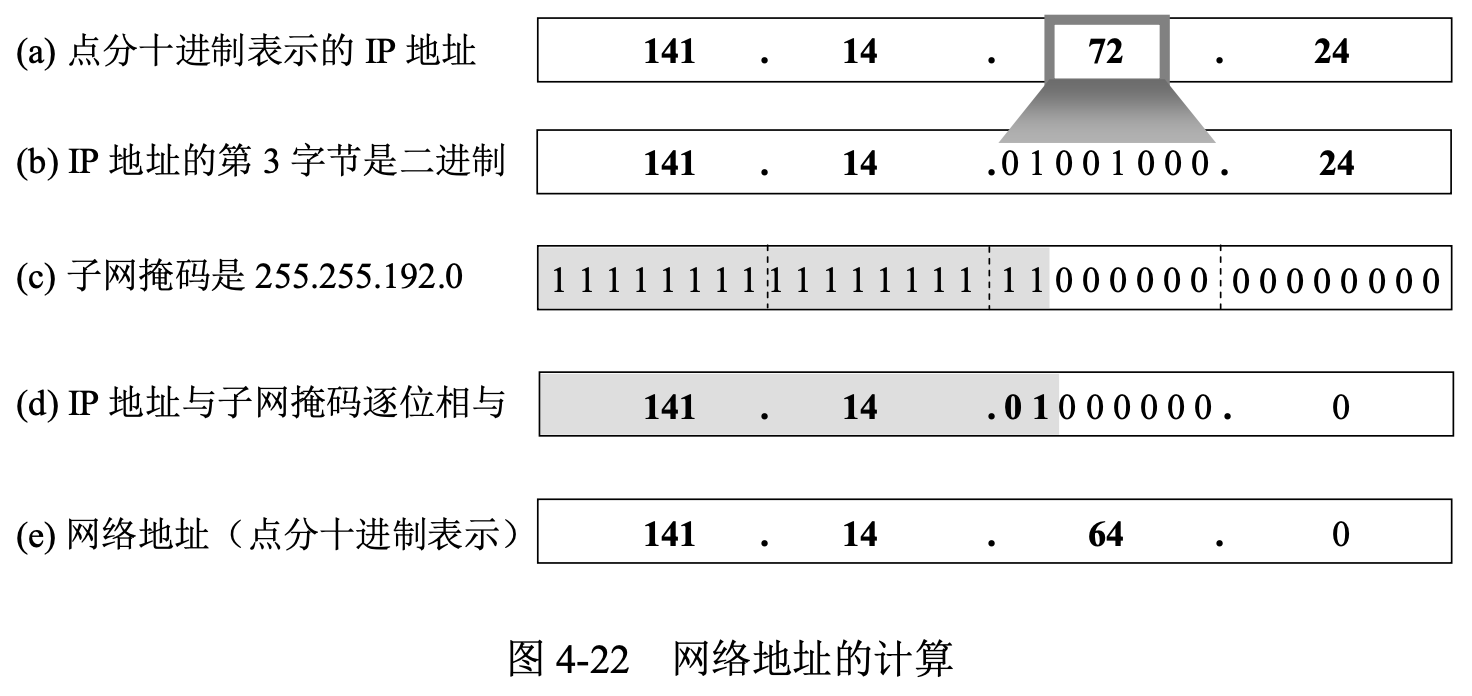
\includegraphics[width=0.65\textwidth]{img/4.22}
	\end{figure}


	\subsection{使用子网时分组的转发}
	在划分子网的情况下,路由器转发分组的算法如下:
	\begin{enumerate}[label=\arabic*.]
		\item 从收到的数据报的首部提取目的 IP 地址 $D$
		\item 先判断是否为直接交付。对路由器直接相连的网络逐个进行检查:用各网络的子网掩码和 $D$ 逐位相“与”,看结果是否和相应的网络地址匹配。若匹配,则把分组进行直接交付(当然还需要把 $D$ 转换成物理地址,把数据报封装成帧发送出去),转发任务结束。否则就是间接交付,执行3
		\item 若路由表中有目的地址为 $D$ 的特定主机路由,则把数据报传送给路由表中所指明的下一跳路由器;否则,执行4
		\item 对路由表中的每一行(目的网络地址,子网掩码,下一跳地址),用其中的子网掩码和 $D$ 逐位相“与”,其结果为 $N$。若 $N$ 与该行的目的网络地址匹配,则把数据报传送给该行指明的下一跳路由器;否则,执行5
		\item 若路由表中有一个默认路由,则把数据报传送给路由表中所指明的默认路由器;否则,执行6
		\item 报告转发分组出错
	\end{enumerate}

	\textbf{例:}源主机 $H_1$ 向目的主机 $H_2$ 发送分组。试讨论 $R_1$ 收到 $H_1$ 向 $H_2$ 发送的分组后查找路由表的过程
	\begin{figure}[H]
		\centering
		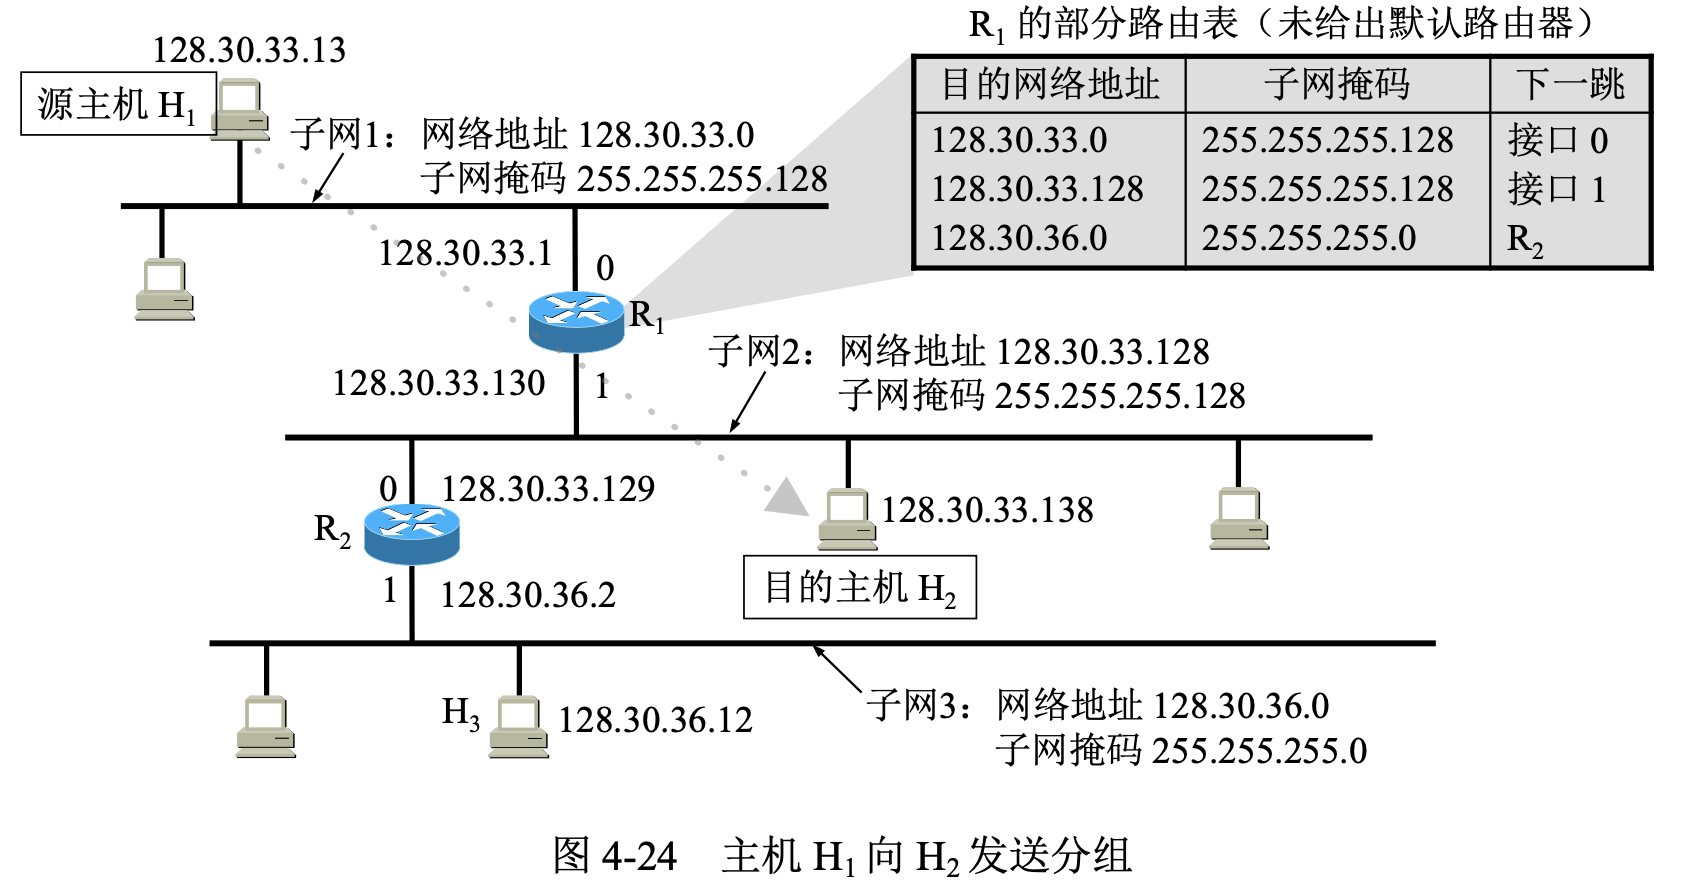
\includegraphics[width=0.7\textwidth]{img/4.24}
	\end{figure}

	\begin{itemize}
		\item 源主机 $H_1$ 把本子网的“子网掩码 255.255.255.128”与目的主机 $H_2$ 的“IP 地址 128.30.33.138”逐位相“与”,得出 128.30.33.128,它不等于 $H_1$ 的 网络地址(128.30.33.0)。这说明 $H_2$ 与$H_1$ 不在同一个子网上。因此 $H_1$ 不能把分组直接交付 $H_2$,而必须交给子网上的默认路由器 $R_1$,由 $R_1$ 来转发。
		\item 路由器 $R_1$ 在收到一个分组后,就在其路由表中逐行寻找有无匹配的网络地址。
		\item 先看 $R_1$ 路由表中的第一行。用这一行的“子网掩码 255.255.255.128”和收到的分组的 “目的地址 128.30.33.138”逐位相“与”,得出 128.30.33.128。然后和这一行给出的目的网络地址 128.30.33.0 进行比较。但比较的结果不一致(即不匹配)。
		\item 用同样方法继续往下找第二行。用第二行的“子网掩码 255.255.255.128”和该分组的 “目的地址 128.30.33.138”逐位相“与”,结果也是 128.30.33.128。这个结果和第二行的目的网络地址 128.30.33.\\128 相匹配,说明这个网络就是收到的分组所要寻找的目的网络。于是不需要再继续查找下去。$R_1$ 把分组从接口 1 直接交付主机 $H_2$。
	\end{itemize}

	\subsection{无分类编址CIDR(构造超网)}

	\subsubsection{网络前缀}
	\begin{itemize}
		\item 划分子网在一定程度上缓解了因特网在发展中遇到的困难,但是数量巨大的 C 类网因为其地址空间太小并没有得到充分使用,而因特网的 IP 地址仍在加速消耗,整个 IPv4 地址空间面临全部耗尽的威胁
		\item 为此,因特网工程任务组 IETF 又提出了采用无分类编制的方法来解决 IP 地址紧张的问题,同时还专门成立 IPv6 工作组负责研究新版本 IP 以彻底解决 IP 地址耗尽的问题
		\item 1993年,IETF 发布了无分类域间路由选择 CIDR(classless inter-domain routing)的 RFC 文档 RFC 1517$\sim$ 1519和1520
		\begin{itemize}
			\item CIDR 消除了传统的 A 类、B 类和 C 类地址,以及划分子网概念
			\item CIDR 可以更加有效地分配 IPv4 的地址空间,并且可以在新的 IPv6 使用之前允许因特网的规模继续增长
		\end{itemize}
		\item CIDR 使用“斜线记法”或称为 CIDR 记法,即在 IPv4 地址后面加上斜线“/”,在斜线后面写上网络前缀所占的比特数量
		\begin{itemize}
			\item 例如 128.14.35.7/20 表示网络前缀所占用的比特数量为 20,主机编号所占用的比特数量为 12
		\end{itemize}
		\item CIDR 实际上是将网络前缀都相同的连续的 IP 地址组成一个“CIDR 地址块”
	\end{itemize}

	\textbf{例:}请给出 CIDR 地址块128.14.35.7/20 的全部细节
	\begin{figure}[H]
		\centering
		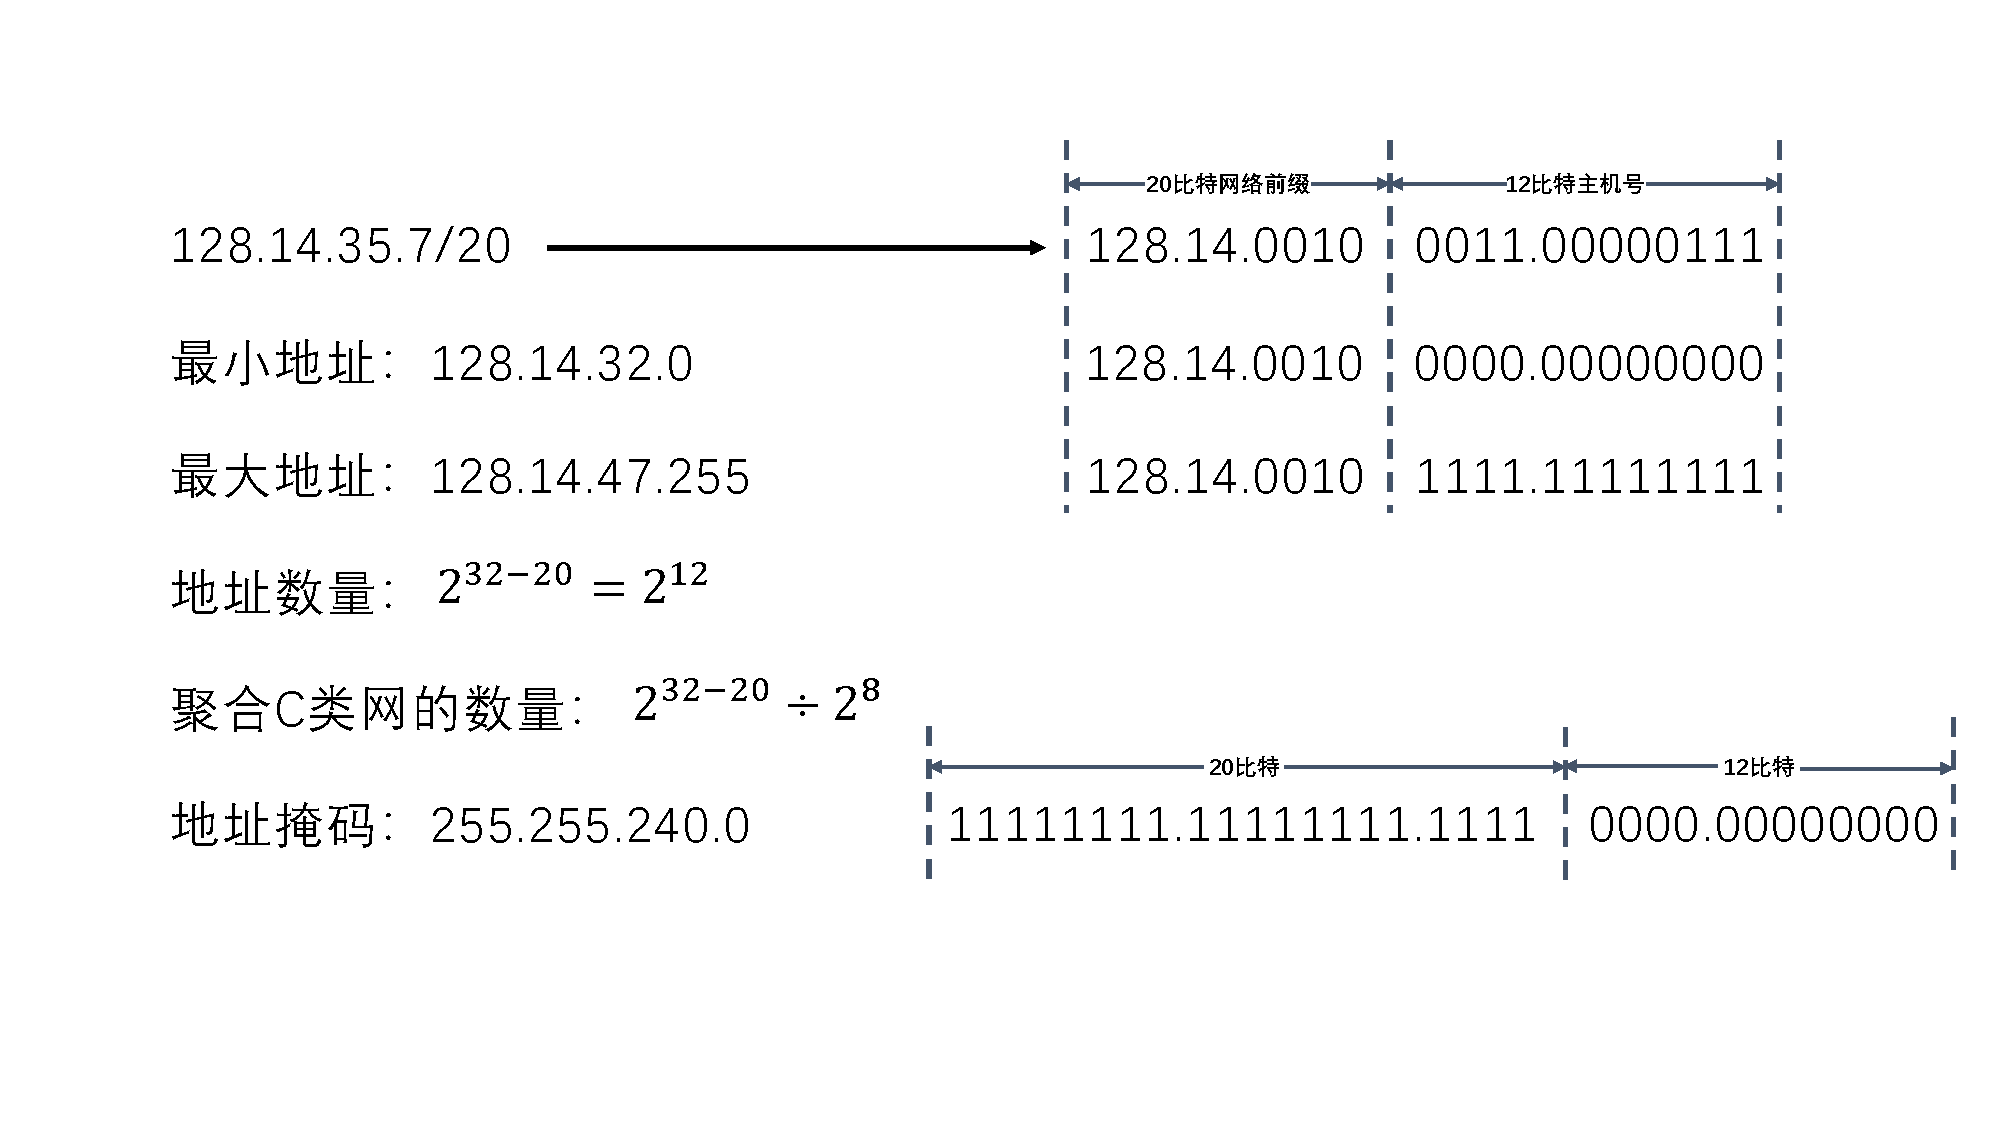
\includegraphics[width=0.65\textwidth]{img/4.3.3.1}
	\end{figure}

	\subsubsection{最长前缀匹配}
	\begin{itemize}
		\item 在使用 CIDR 时,由于采用了网络前缀这种记法,因此在路由表中的项目需要改变为由“网络前缀”和 “下一跳地址”组成。但是在查找路由表时可能会得到不止一个匹配结果
		\item 对于这种情况,应当从匹配结果中选择具有最长网络前缀的路由。这叫做最长前缀匹配(longest-prefix matching)
		\item 这是因为网络前缀越长,其地址块就越小,因而路由就越具体
	\end{itemize}

	\begin{figure}[H]
		\centering
		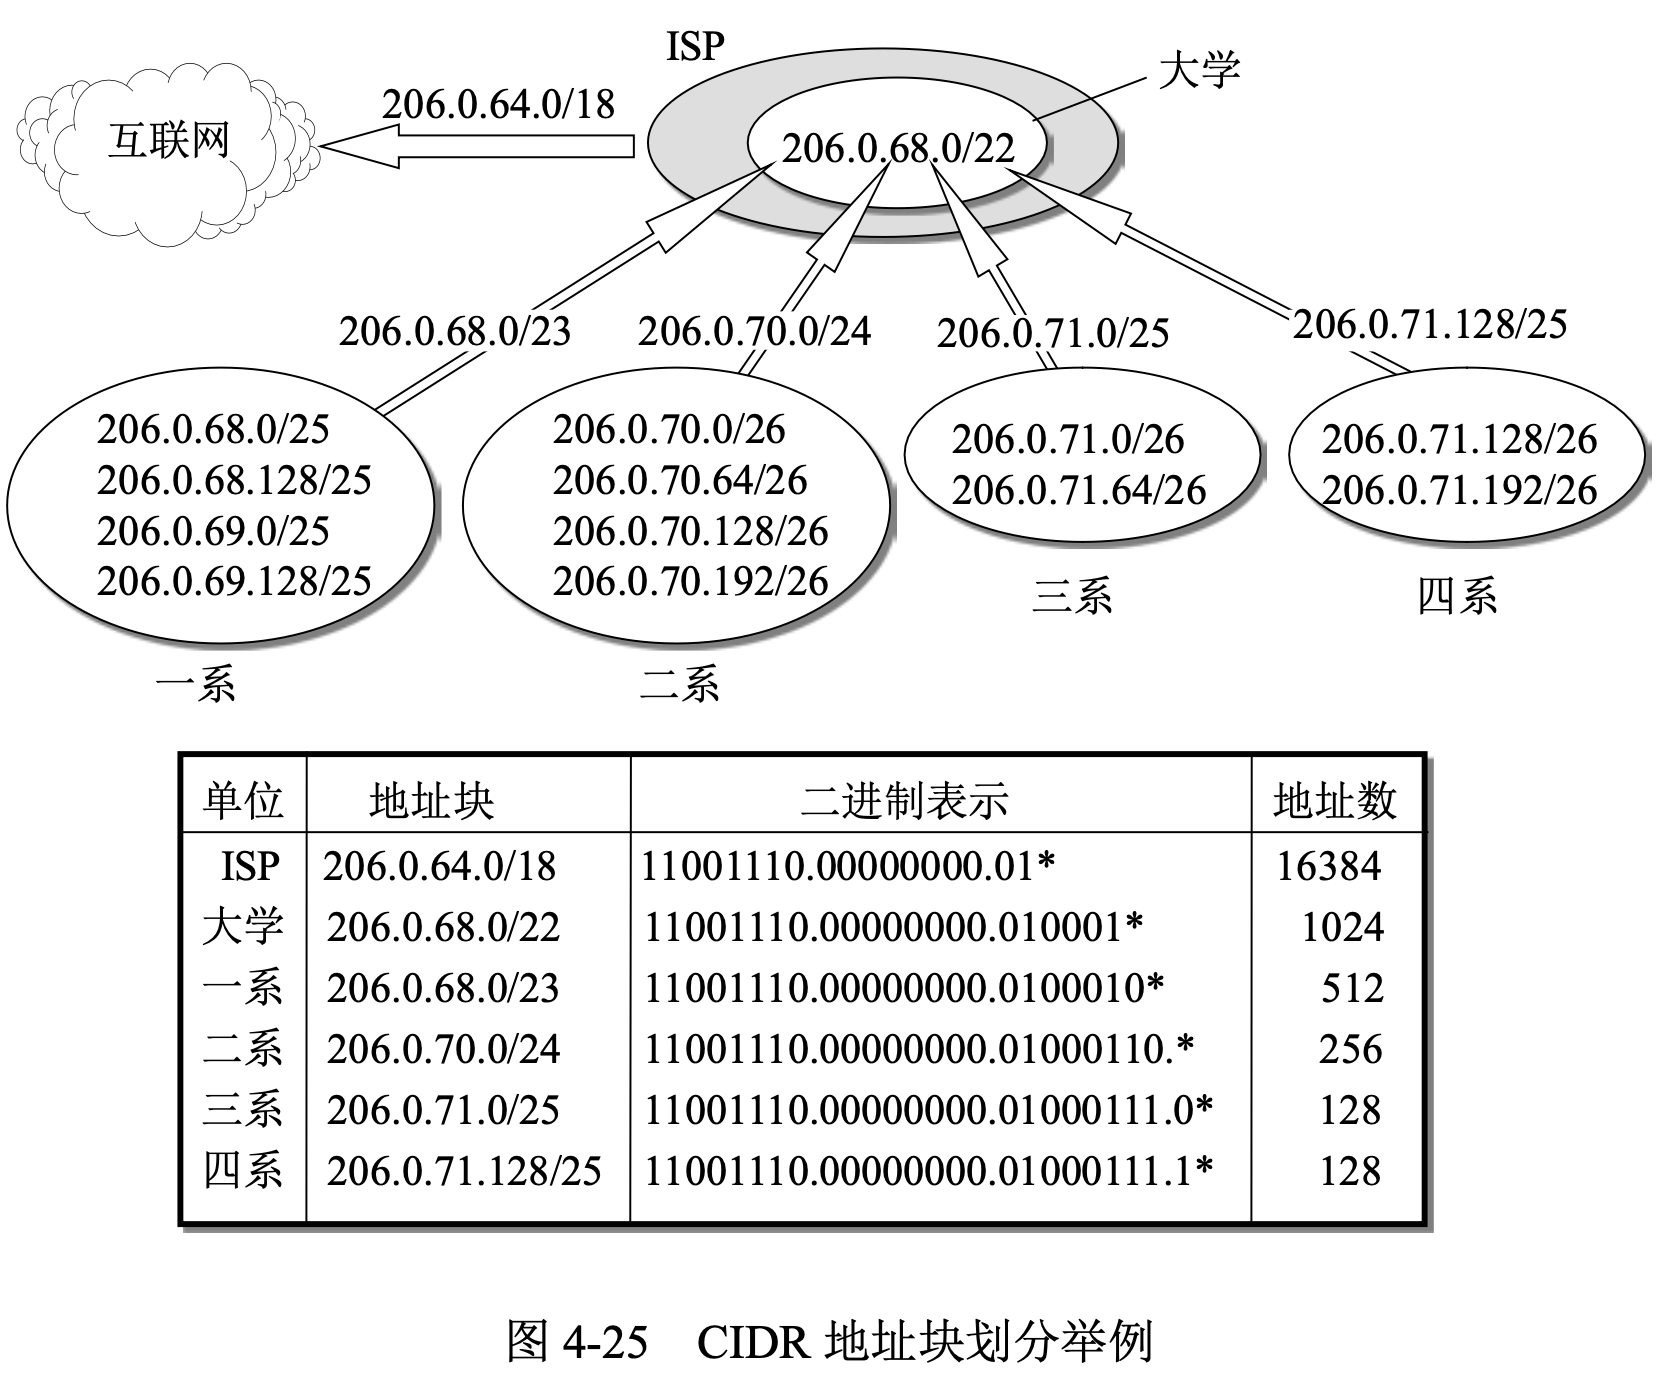
\includegraphics[width=0.55\textwidth]{img/4.25}
	\end{figure}

	例如,对于上图中假定 ISP 收到一个数据报,其目的地址 IP 为 $D=$206.0.71.130,把 $D$ 分别和路由表中的大学(206.0.68.0/22)和四系(206.0.71.128/25)的子网掩码诸位相“与”,发现均匹配,但根据最长前缀原则,应该选择后者(四系)

	\section{网际控制报文协议ICMP}
	\begin{itemize}
		\item 为了更有效地转发 IP 数据报和提高交付成功的机会,在网际层使用了网际控制报文协议 ICMP(Internet Control Message Protocol)
		\item ICMP 报文被封装在 IP 数据报中发送
	\end{itemize}
	\begin{figure}[H]
		\centering
		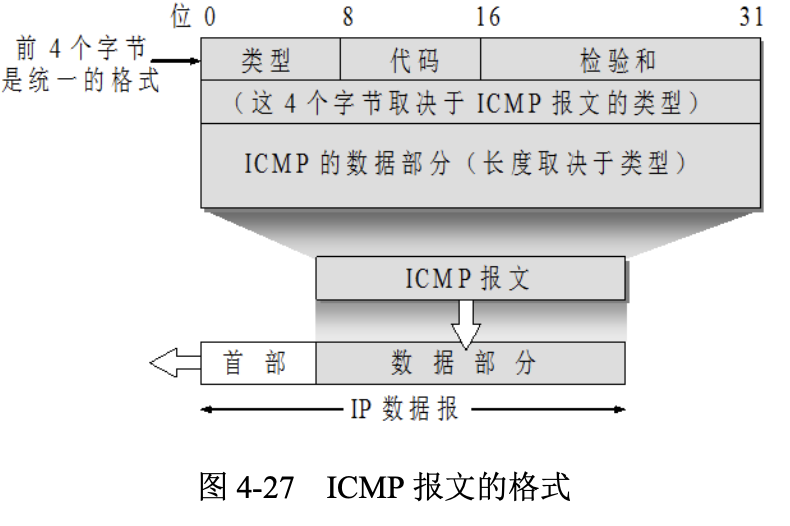
\includegraphics[width=0.5\textwidth]{img/4.27}
	\end{figure}

	\subsection{ICMP报文的种类}
	ICMP 报文的种类有两种,即 ICMP 差错报告报文和 ICMP 询问报文
	\begin{itemize}
		\item ICMP 差错报告报文共有以下五种:
		\begin{itemize}
			\item 终点不可达:当路由器或主机不能交付数据报时,就向源点发送终点不可达报文。具体可再根据 ICMP 的代码字段细分为目的网络不可达、目的主机不可达、目的端口不可达、目的网络未知、目的主机未知等13种错误
			\item 源点抑制:当路由器或主机由于拥塞而丢弃数据报时,就向源点发送源点抑制报文,使源点知道应当把数据报的发送速率放慢
			\item 时间超过:当路由器收到一个目的 IP 地址不是自己的 IP 数据报,会将其生存时间 TTL 字段的值减 1,若结果不为 0,则将该 IP 数据报转发出去;若结果为 0,除丢弃该 IP 数据报外,还要向源点发送时间超过报文。另外,当终点在预先规定的时间内不能收到一个数据报的全部数据报片时,就把已收到的数据报片都丢弃,也会向源点发送时间超过报文
			\item 参数问题:当路由器或目的主机收到 IP 数据报后,根据其首部中的检验和字段发现首部在传输过程中出现了误码,就丢弃该数据报,并向源点发送参数问题报文
			\item 改变路由(重定向):路由器把改变路由报文发送给主机,让主机知道下次应将数据报发送给另外的路由器(可通过更好的路由)
		\end{itemize}
		\item 以下情况下不应发送 ICMP 差错报告报文:
		\begin{itemize}
			\item 对 ICMP 差错报告报文,不再发送 ICMP 差错报告报文
			\item 对第一个分片的数据报片的所有后续数据报片,都不发送 ICMP 差错报告报文
			\item 对具有多播地址的数据报,都不发送 ICMP 差错报告报文
			\item 对具有特殊地址(如 127.0.0.0 或 0.0.0.0)的数据报,不发送 ICMP 差错报告报文
		\end{itemize}
		\item 常用的 ICMP 询问报文有两种:
		\begin{itemize}
			\item 回送请求和回答: ICMP 回送请求报文是由主机或路由器向一个特定的目的主机发出的询问。收到此报文的主机必须给源主机或路由器发送 ICMP 回送回答报文。这种询问报文用来测试目的站是否可达以及了解其有关状态
			\item 时间戳请求和回答: ICMP 时间戳请求报文是请某台主机或路由器回答当前的日 期和时间。在 ICMP 时间戳回答报文中有一个 32 位的字段,其中写入的整数代表从 1900 年 1 月 1 日起到当前时刻一共有多少秒。时间戳请求与回答可用于时钟同步和时间测量
		\end{itemize}
	\end{itemize}

	\subsection{ICMP的应用举例}
	\begin{itemize}
		\item 分组网间探测 PING(Packet InterNet Groper)
		\begin{itemize}
			\item 用来测试主机和路由器间的连通性
			\item 应用层直接使用网际层的 ICMP(没有通过运输层的 TCP 或 UDP)
			\item 使用 ICMP 回送请求和回答报文
			\item 使用命令为\ \verb|ping hostname|
		\end{itemize}
		\item 跟踪路由(traceroute)
		\begin{itemize}
			\item 用来测试 IP 数据报从源主机到达目的主机需要经过哪些路由器
			\item Windows 版本
			\begin{itemize}
				\item \verb|tracert|\ 命令
				\item 应用层直接使用网际层 ICMP
				\item 使用了 ICMP 回送请求和回答报文以及差错报告报文
			\end{itemize}
			\item Unix 版本
			\begin{itemize}
				\item \verb|traceroute|\ 命令
				\item 在运输层使用 UDP 协议
				\item 仅使用 ICMP 差错报告报文
			\end{itemize}
		\end{itemize}
	\end{itemize}

	\section{互联网的路由选择协议}

	\subsection{有关路由选择协议的几个基本概念}

	\subsubsection{理想的路由算法}
	一个理想的路由算法应具有如下的一些特点
	\begin{itemize}
		\item 算法必须是正确的和完整的
		\item 算法在计算上应简单
		\item 算法应能适应通信量和网络拓扑的变化
		\item 算法应具有稳定性
		\item 算法应是公平的
		\item 算法应是最佳的
	\end{itemize}

	倘若从路由算法能否随网络的通信量或拓扑自适应地进行调整变化来划分,则只有两大类,即静态路由选择策略与动态路由选择策略
	\begin{itemize}
		\item 静态路由选择
		\begin{itemize}
			\item 由人工配置的网络路由、默认路由、特定主机路由、黑洞路由等都属于静态路由
			\item 这种人工配置方式简单、开销小,但不能及时适应网络状态(流量、拓扑等)的变化
			\item 一般只在小规模网络中采用
		\end{itemize}
		\item 动态路由选择
		\begin{itemize}
			\item 路由器通过路由选择协议自动获取路由信息
			\item 比较复杂、开销比较大,能较好地适应网络状态的变化
			\item 适用于大规模网络
		\end{itemize}
	\end{itemize}

	\subsubsection{分层次的路由选择协议}
	互联网采用分层次的路由选择协议,因此可以把整个互联网划分为许多较小的自治系统 AS(autonomous system)。自治系统 AS 是在单一技术管理下的一组路由器,而这些路由器使用一种自治系统内部的路由选择协议和共同的度量。一个 AS 对其他 AS 表现出的是一个单一的和一致的路由选择策略
	\begin{figure}[H]
		\centering
		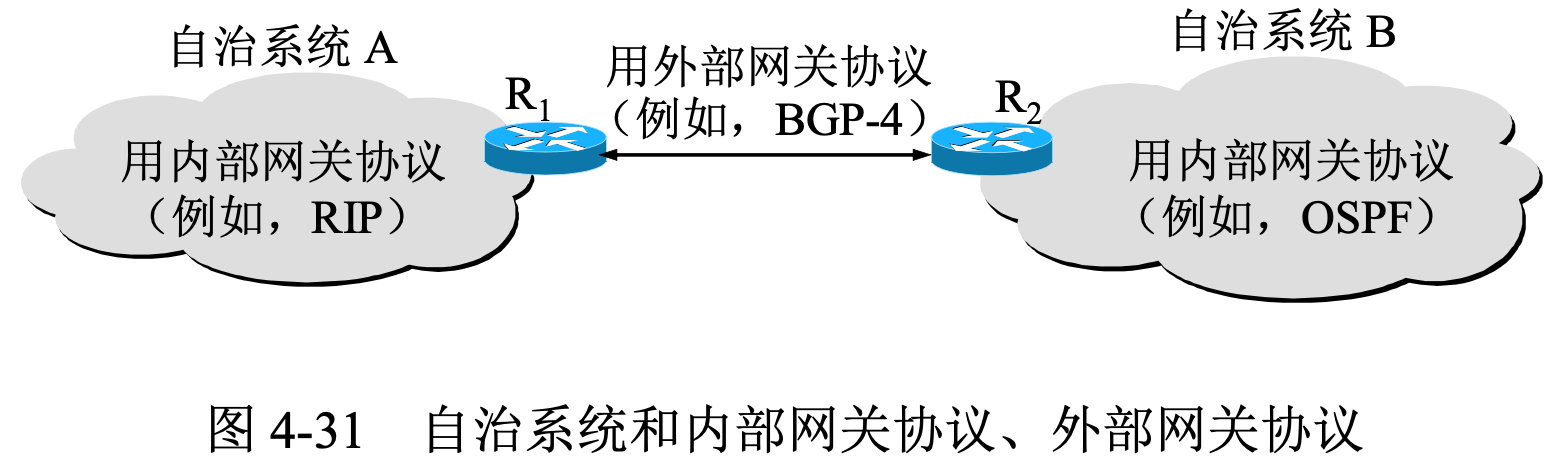
\includegraphics[width=0.65\textwidth]{img/4.31}
	\end{figure}

	互联网将路由选择协议划分为两大类,即:
	\begin{itemize}
		\item 内部网关协议 IGP(Interior Gateway Protocol):即在一个自治系统内部使用的路由选择协议,而这与在互联网中的其他自治系统选用什么路由选择协议无关。目前这类路由选择协议使用得最多,如 RIP 和 OSPF 协议
		\item 外部网关协议 EGP(External Gateway Protocol):若源主机和目的主机处在不同的自治系统中(这两个自治系统可能使用不同的内部网关协议),当数据报传到一个自治系统的边界时,就需要使用一种协议将路由选择信息传递到另一个自治系统中。这样的协议就是外部网关协议 EGP。目前使用最多的外部网关协议是 BGP 的版本 4(BGP-4)
	\end{itemize}

	\begin{figure}[H]
		\centering
		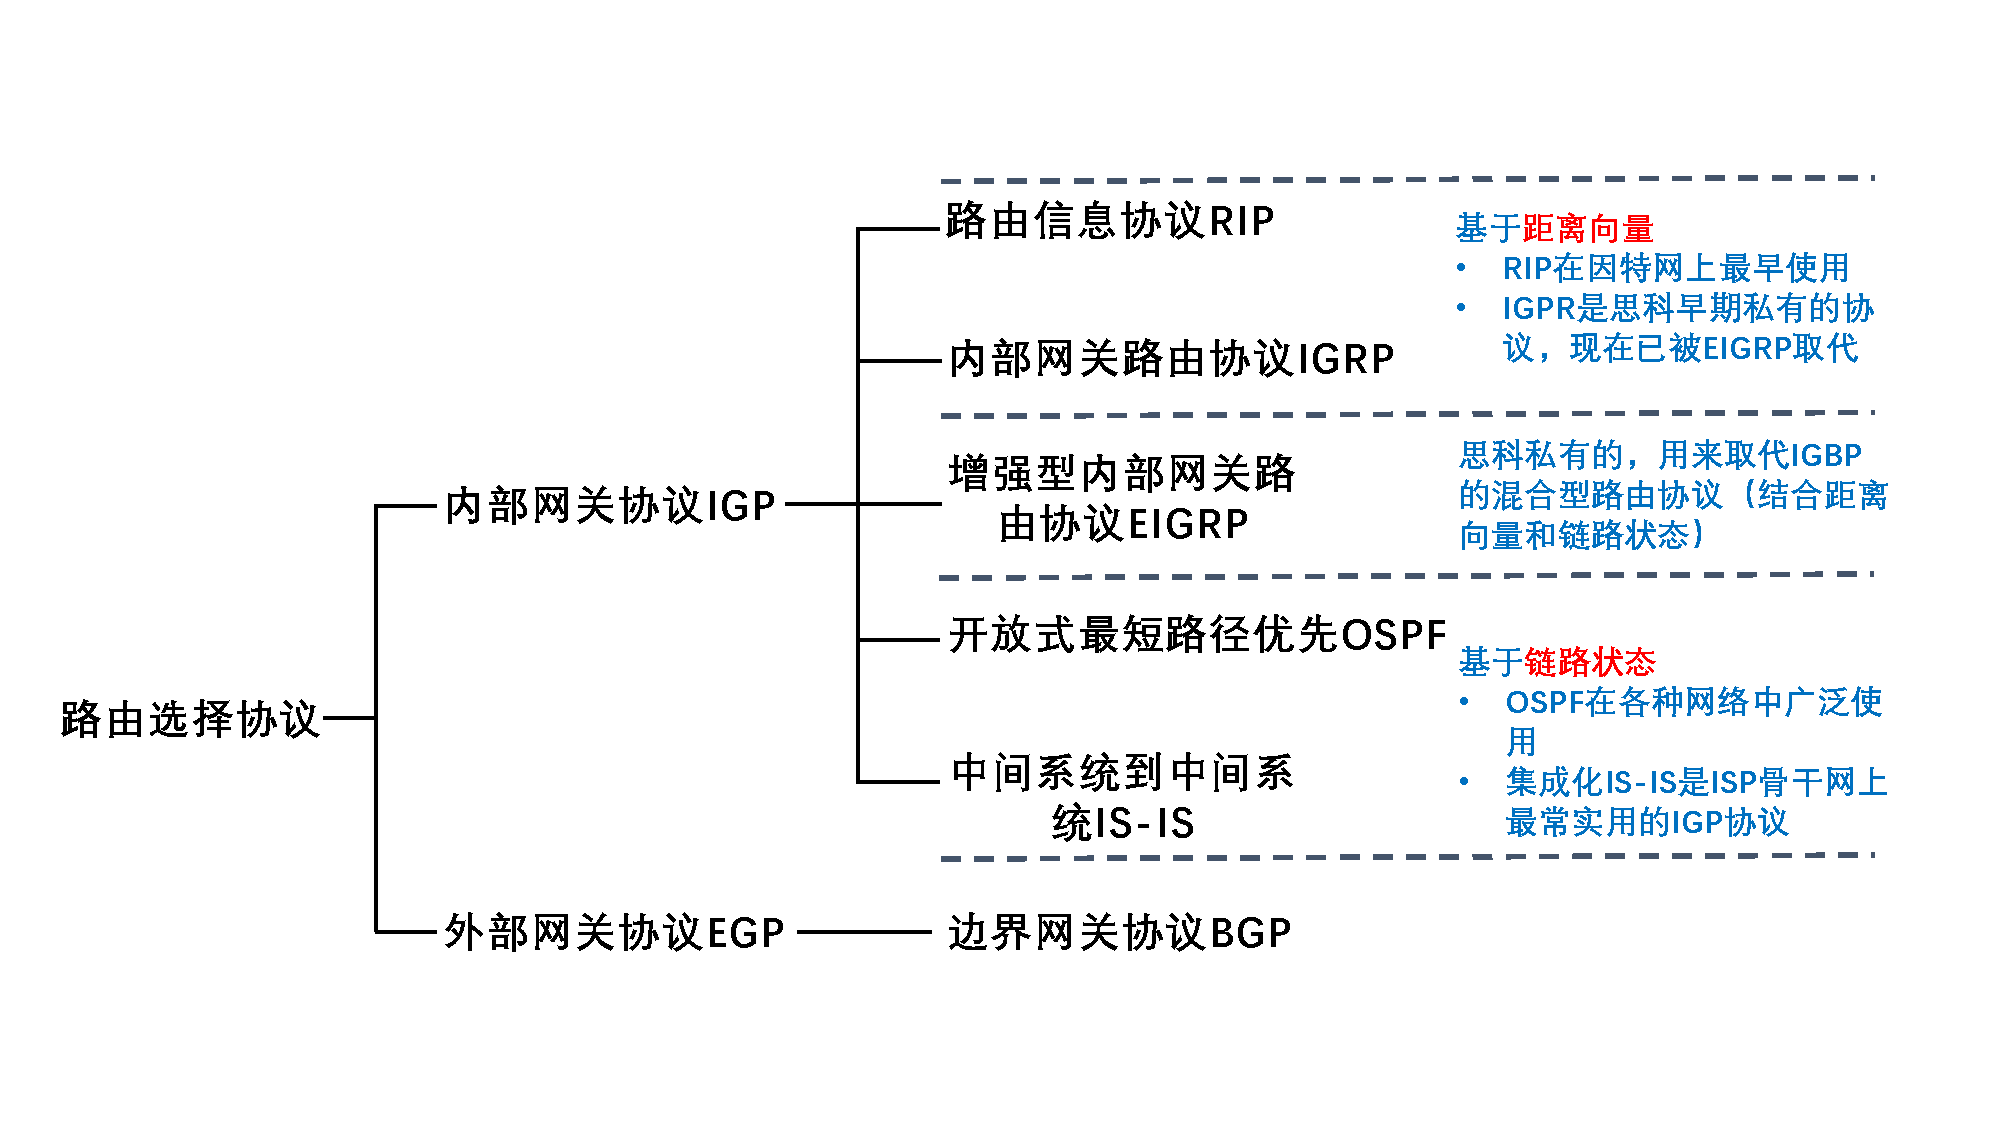
\includegraphics[width=0.8\textwidth]{img/4.5.2}
	\end{figure}

	\subsection{内部网关协议RIP}

	\subsubsection{工作原理}
	\begin{itemize}
		\item 路由信息协议 RIP(routing information protocol)是内部网关协议 IGP 中最先得到广泛使用的协议之一,其相关标准文档为 RFC 1058
		\item RIP 要求自治系统 AS 内的每一个路由器都要维护从它自己到 AS 内其他每一个网络的距离记录。这是一组距离,称为距离向量 D-V(distance vector)
		\item RIP 使用跳数(hop count)作为度量(metric)来衡量到达目的网络的距离
		\begin{itemize}
			\item 路由器到直连网络的距离定义为 1
			\item 路由器到非直连网络的距离定义为所经过的路由器数加 1
			\item 允许一条路径最多只能包含 15 个路由器。“距离”等于 16 时相当于不可达。因此 RIP 只适用于小型互联网
		\end{itemize}
		\item RIP 认为好的路由就是“距离短”的路由,也就是所通过路由器数量最少的路由
		\item 当到达同一目的网络有多条“距离相等”的路由时,可以进行等价负载均衡
		\item RIP 包含以下三个要点:
		\begin{itemize}
			\item 和谁交换信息:仅和相邻路由器交换信息
			\item 交换什么信息:当前本路由器所知道的全部信息,即自己现在的路由表
			\item 在什么时候交换信息:按固定的时间间隔周期性交换(例如每 30 秒)
		\end{itemize}
		\item 路由器在刚刚开始工作时,它的路由表是空的。然后路由器就得出到直接相连的几个网络的距离(这些距离定义为 1)。接着,每一个路由器也只和数目非常有限的相邻路由器交换并更新路由信息。但经过若干次的更新后,所有的路由器最终都会知道到达本自治系统中任何一个网络的最短距离和下一跳路由器的地址
	\end{itemize}

	\subsubsection{距离向量算法}
	对每一个相邻路由器发送过来的 RIP 报文,进行以下步骤:
	\begin{enumerate}[label=\arabic*.]
		\item 对地址为 $X$ 的相邻路由器发来的 RIP 报文,先修改此报文中的所有项目:把“下一跳”字段中的地址都改为 $X$,并把所有的“距离”字段的值加 1。每一个项目都有三个关键数据,即:到目的网络 $N$,距离是 $d$,下一跳路由器是 $X$
		\item 对修改后的 RIP 报文中的每一个项目,进行以下步骤: 
		\begin{itemize}
			\item 若原来的路由表中没有目的网络 $N$,则把该项目添加到路由表中
			\item 否则(即在路由表中有目的网络 $N$,这时就再查看下一跳路由器地址)
			\begin{itemize}
				\item 若下一跳路由器地址是 $X$,则把收到的项目替换原路由表中的项目 
				\item 否则(即这个项目是到目的网络 $N$,但下一跳路由器不是 $X$)
				\begin{itemize}
					\item 若收到的项目中的距离 $d$ 小于路由表中的距离,则进行更新
					\item 否则什么也不做
				\end{itemize}
			\end{itemize}
		\end{itemize}
		\item 若 3 分钟还没有收到相邻路由器的更新路由表,则把此相邻路由器记为不可达的路路由器,即把距离置为 16(距离为 16 表示不可达)
		\item 返回
	\end{enumerate}

	已知路由器 $R_6$ 有下表所示的路由表。现在收到相邻路由器 $R_4$ 发来的路由更新信息,如下表所示。试更新路由器 $R_6$ 的路由表

	路由器 $R_6$ 的路由表(表1)
	\begin{table}[H]
		\centering
		\begin{tabular}{|c|c|c|}
		\hline
		目的网络  & 距离 & 下一跳路由器 \\ \hline
		Net 2 & 3  & $R_4$  \\ \hline
		Net 3 & 4  & $R_5$  \\ \hline
		……    & …… & ……     \\ \hline
		\end{tabular}
	\end{table}

	$R_4$ 发来的路由更新信息(表2)
	\begin{table}[H]
		\centering
		\begin{tabular}{|c|c|c|}
		\hline
		目的网络  & 距离 & 下一跳路由器 \\ \hline
		Net 1 & 3  & $R_1$  \\ \hline
		Net 2 & 4  & $R_2$  \\ \hline
		Net 3 & 1  & 直接交付   \\ \hline
		\end{tabular}
	\end{table}

	首先先把表2中的距离都加1,并把下一跳路由器都改为 $R_4$,得出表3
	\begin{table}[H]
		\centering
		\begin{tabular}{|c|c|c|}
		\hline
		目的网络  & 距离 & 下一跳路由器 \\ \hline
		Net 1 & 4  & $R_4$  \\ \hline
		Net 2 & 5  & $R_4$  \\ \hline
		Net 3 & 2  & $R_4$  \\ \hline
		\end{tabular}
	\end{table}

	把表3和的每一行和表1进行比较
	\begin{itemize}
		\item 第一行在表1中没有,因此要把这一行添加到表1中
		\item 第二行的 Net 2 在表1中有,且下一跳路由器也是 $R_4$。因此要更新(最新消息)
		\item 第三行的 Net 3 在表1中有,但下一跳路由器不同。于是就要比较距离。新的路由信息的距离是 2,小于原来表中的 4,因此要更新
	\end{itemize}

	得出更新后的 R6 的路由表如下表所示
	\begin{table}[H]
		\centering
		\begin{tabular}{|c|c|c|}
		\hline
		目的网络  & 距离 & 下一跳路由器 \\ \hline
		Net 1 & 4  & $R_4$  \\ \hline
		Net 2 & 5  & $R_4$  \\ \hline
		Net 3 & 2  & $R_4$  \\ \hline
		……    & …… & ……     \\ \hline
		\end{tabular}
	\end{table}

	\subsubsection{RIP协议的报文格式}
	\begin{figure}[H]
		\centering
		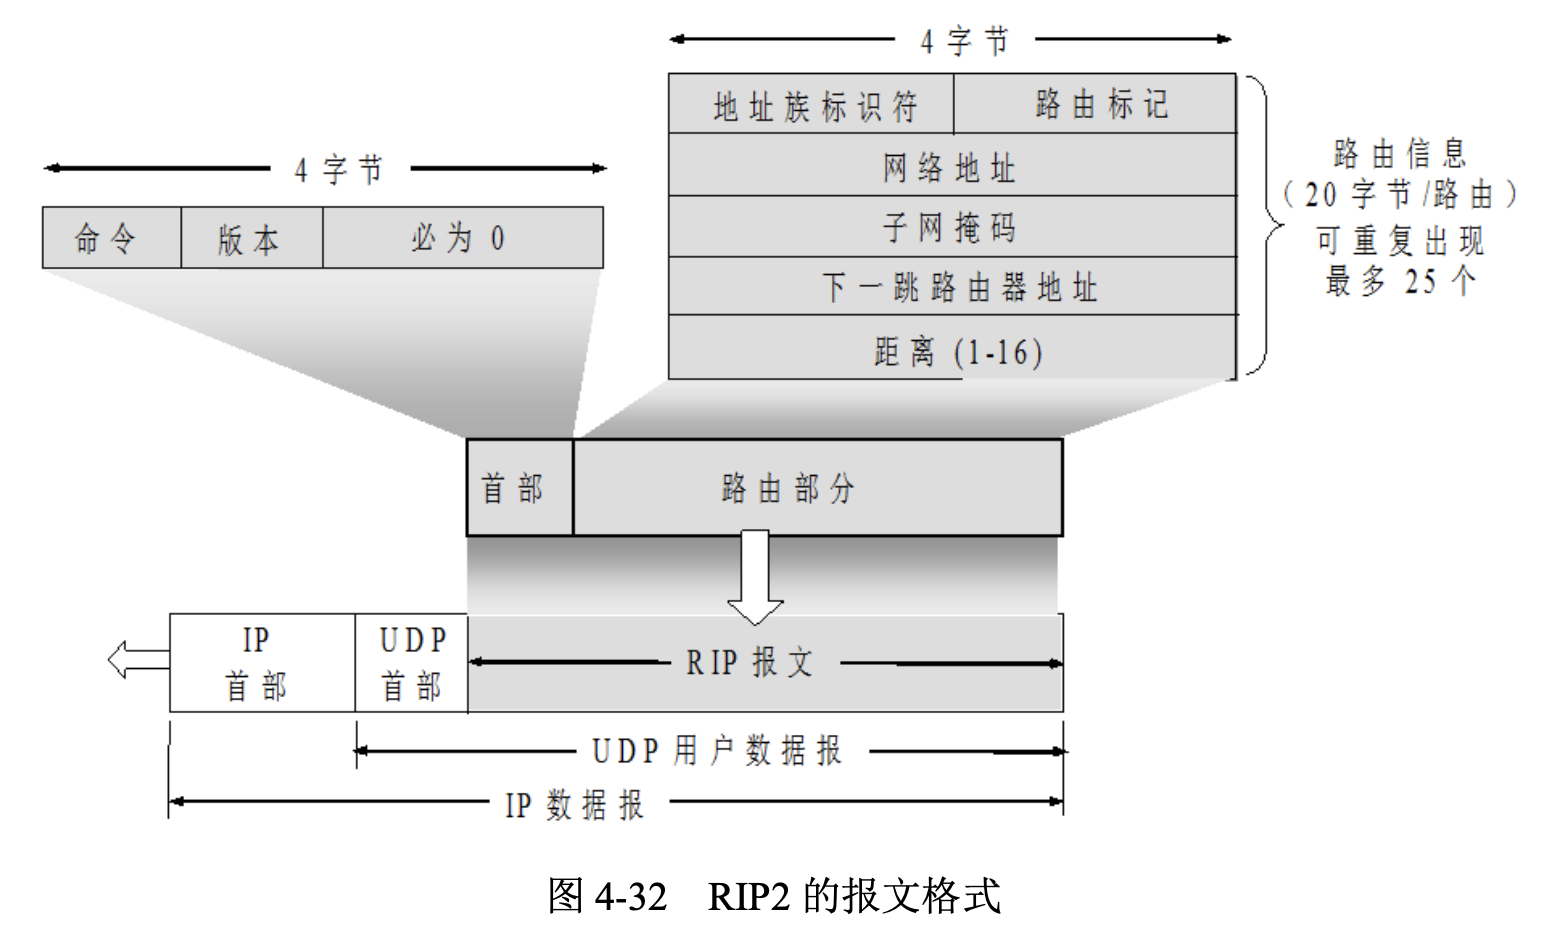
\includegraphics[width=0.7\textwidth]{img/4.32}
	\end{figure}

	\begin{itemize}
		\item RIP 存在“坏消息传播得慢”的问题,即当网络出现故障时,要经过比较长的时间才能将此信息传送到所有的路由器
		\item “坏消息传播得慢”又称为路由环路或距离无穷计数问题,这是距离向量算法的一个固有问题。可以采取多种措施减少出现该问题的概率或减小该问题带来的危害
		\begin{itemize}
			\item 限制最大路径距离为 15(16表示不可达)
			\item 当路由表发生变化时就立即发送更新报文(即“触发更新”),而不仅是周期性发送
			\item 让路由器记录收到某特定路由信息的接口,而不让同一路由信息再通过此接口向反方向传送(即“水平分割”)
		\end{itemize}
	\end{itemize}

	\begin{figure}[H]
		\centering
		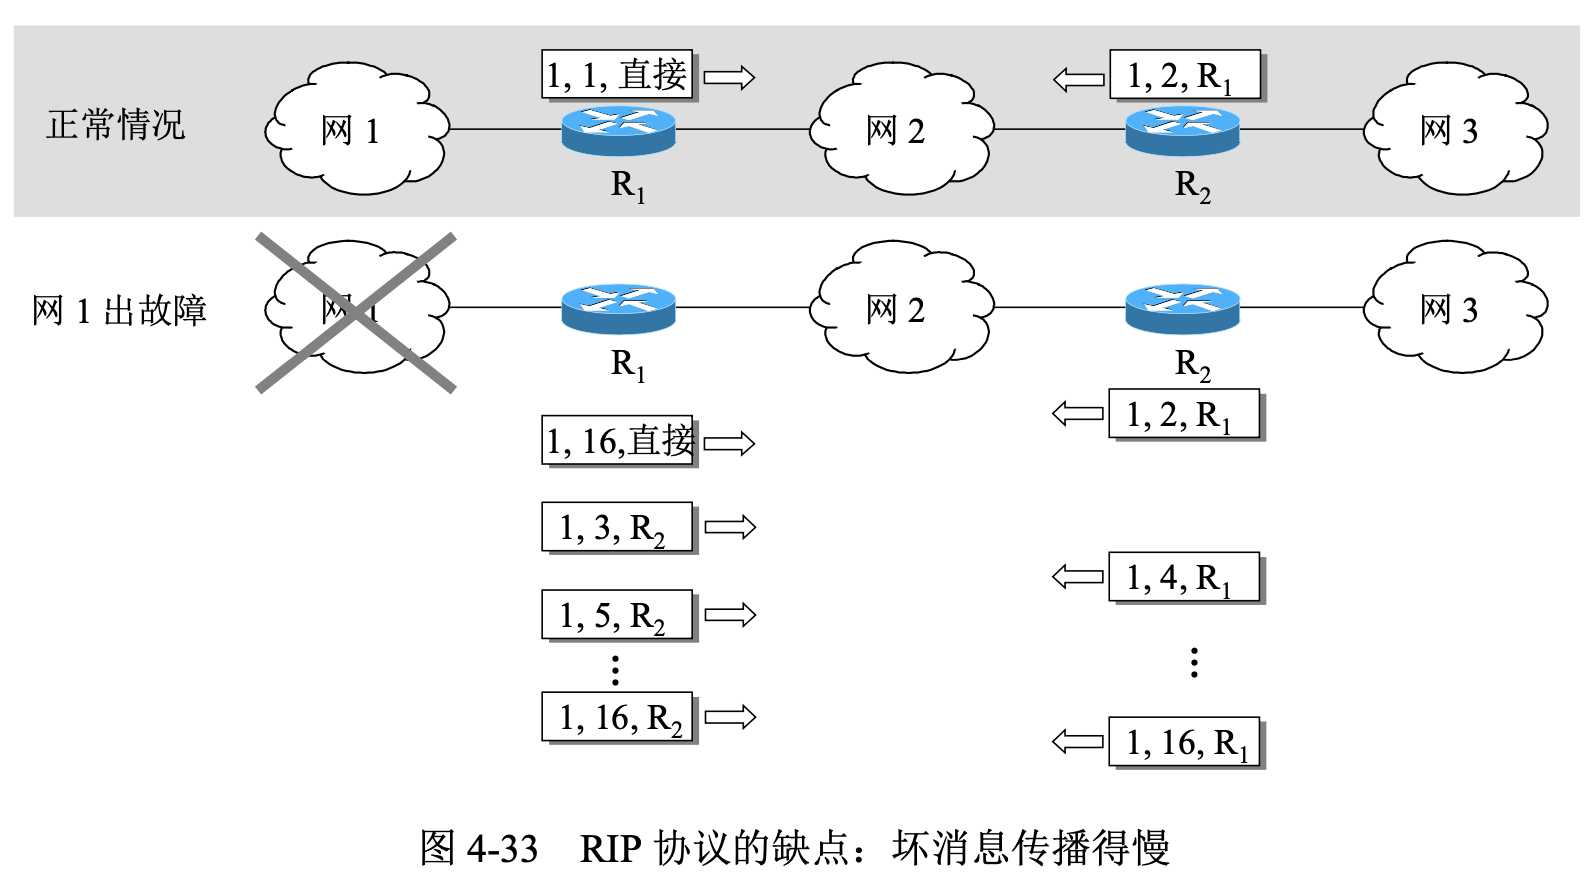
\includegraphics[width=0.7\textwidth]{img/4.33}
	\end{figure}
	\begin{itemize}
		\item 现在假定路由器 $R_1$ 到网 1 的链路出了故障,$R_1$ 无法到达网 1。于是路由器 $R_1$ 把到网 1 的距离改为 16(表示到网 1 不可达),因而在 $R_1$ 的路由表中的相应项目变为“1, 16, 直接”
		\item 但是,很可能要经过 30 秒钟后 $R_1$ 才把更新信息发送给 $R_2$。然而 $R_2$ 可能已经先把自己的路由表发送给了 $R_1$,其中有“1, 2, $R_1$”这一项
		\item $R_1$ 收到 $R_2$ 的更新报文后,误认为可经过 $R_2$ 到达网 1,于是把收到的路由信息“1, 2, $R_1$”修改为:“1, 3, $R_2$”,表明“我到网1的距离是3,下一跳经过$R_2$”,并把更新后的信息发送给 $R_2$
		\item 同理,$R_2$ 接着又更新自己的路由表为“1, 4, $R_1$”,以为“我到网1距离是4,下一跳经过 $R_1$”
		\item 这样的更新一直继续下去,直到 $R_1$ 和 $R_2$ 到网 1 的距离都增大到 16 时,$R_1$ 和 $R_2$ 才知道原来网 1 是不可达的
	\end{itemize}

	\subsection{内部网关协议OSPF}

	\subsubsection{OSPF协议的基本特点}
	\begin{itemize}
		\item 开放最短路径优先 OSPF(Open Shortest Path First)是为克服 RIP 的缺点在 1989 年开发出来的
		\begin{itemize}
			\item “开放”表明 OSPF 协议不是受某一家厂商控制,而是公开发表的
			\item “最短路径优先”是因为使用了 Dijkstra 提出的最短路径算法 SPF
		\end{itemize}
		\item OSPF 与 RIP 工作要点的对比
		\begin{itemize}
			\item 采用洪泛法(flooding)向本自治系统中所有路由器发送信息;而 RIP 仅仅向自己相邻的几个路由器发送信息
			\item 发送的信息是与本路由器相邻的所有路由器的链路状态,“链路状态”指的是本路由器都和哪些路由器相邻,以及相应链路的代价(cost);而 RIP 发送的信息是到所有网络的距离和下一跳路由器
			\item 只有当链路状态发生变化时,路由器才向所有路由器用洪泛法发送此信息;而 RIP不管网络拓扑有无发生变化,路由器之间都要定期交换路由表的信息
		\end{itemize}
		\item 由于各路由器之间频繁地交换链路状态信息(link-state advertisement,LSA),因此所有的路由器最终都能建立一个链路状态数据库(link-state database,LSDB),这个数据库实际上就是全网的拓扑结构图,每一个路由器使用链路状态数据库中的数据,构造出自己的路由表
	\end{itemize}

	为了使 OSPF 能够用于规模很大的网络,OSPF 将一个自治系统再划分为若干个更小的范围,叫做区域(area)。划分区域的好处就是把利用洪泛法交换链路状态信息的范围局限于每一个区域而不是整个自治系统,这就减少了整个网络上的通信量

	\begin{figure}[H]
		\centering
		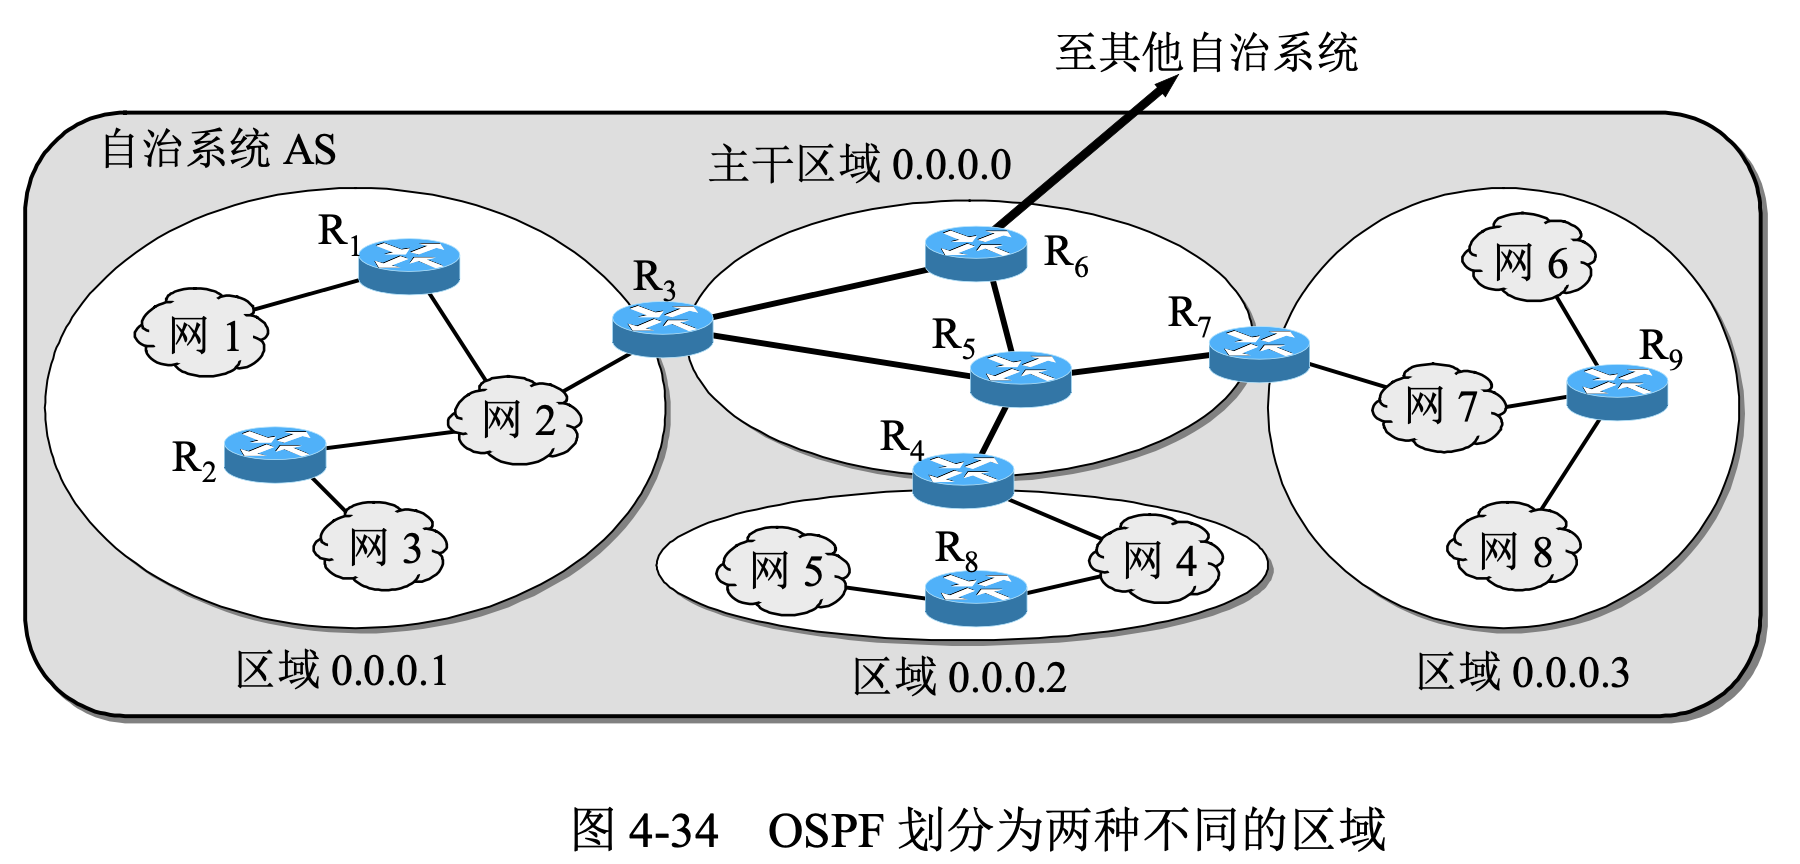
\includegraphics[width=0.7\textwidth]{img/4.34}
	\end{figure}

	对于上图,则有
	\begin{itemize}
		\item 区域内路由器 IR(internal router):$R_1$,$R_2$,$R_8$,$R_9$
		\item 区域边界路由器 ABR(area border router):$R_3$,$R_4$,$R_7$
		\item 主干路由器 BBR(backbone router):$R_3$,$R_4$,$R_5$,$R_6$,$R_7$
		\item 自治系统边界路由器 ASBR(AS border router):$R_6$
	\end{itemize}

	\subsubsection{OSPF的基本工作原理}

	OSPF 共有 5 种分组类型
	\begin{itemize}
		\item 类型 1,问候(Hello)分组,用来发现和维持邻站的可达性
		\item 类型 2,数据库描述(Database Description)分组,向邻站给出自己的链路状态数据库中的所有链路状态项目的摘要信息
		\item 类型 3,链路状态请求(Link State Request)分组,向对方请求发送某些链路状态项目的详细信息
		\item 类型 4,链路状态更新(Link State Update)分组,用洪泛法对全网更新链路状态,路由器使用这种分组将其链路状态通知给邻站
		\item 类型 5,链路状态确认(Link State Acknowledgment)分组,对链路更新分组的确认
	\end{itemize}
	
	\begin{figure}[H]
		\centering
		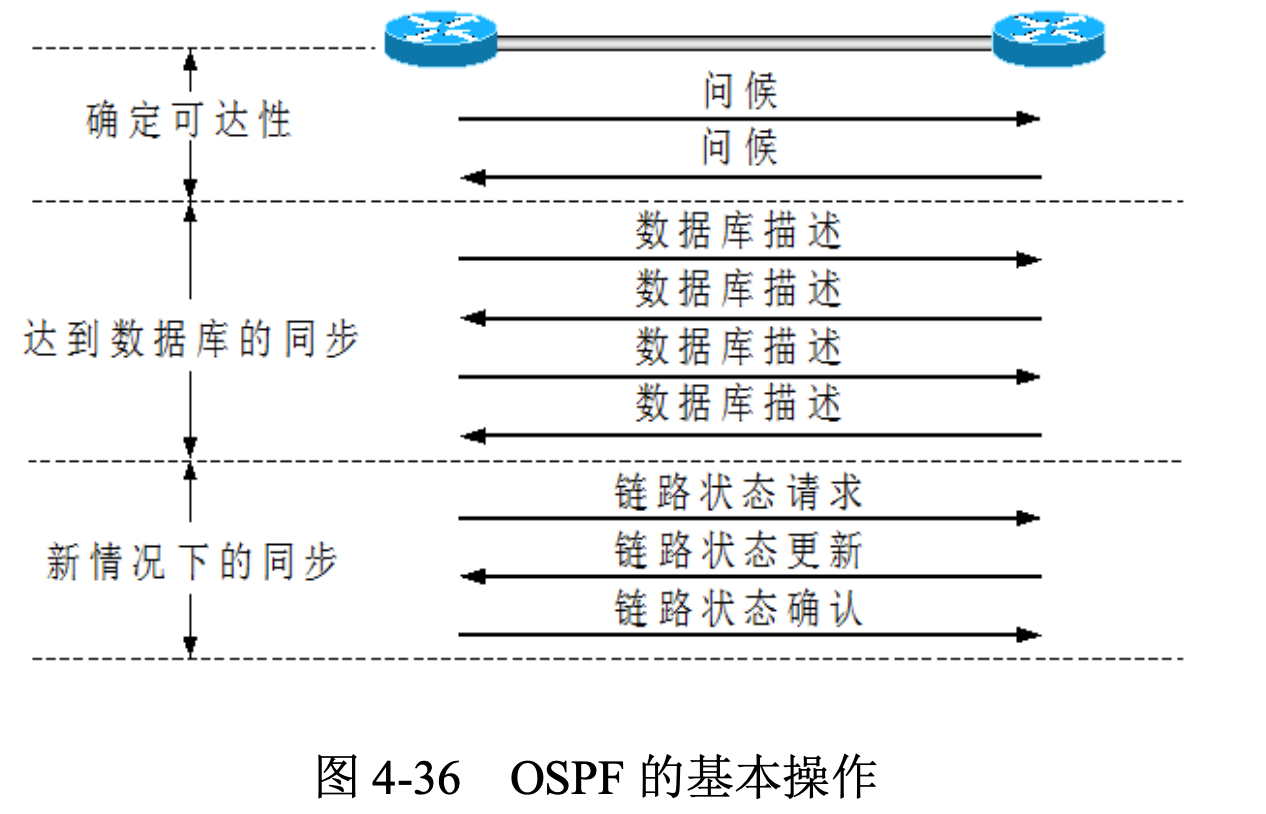
\includegraphics[width=0.55\textwidth]{img/4.36}
	\end{figure}

	\begin{itemize}
		\item OSPF 规定,每两个相邻路由器每隔 10 秒钟要交换一次问候分组。这样就能确知哪些邻站是可达的,若有 40 秒钟没有收到某个相邻路由器发来的问候分组,则可认为该相邻路由器是不可达的,应立即修改链路状态数据库,并重新计算路由表
		\item OSPF 在多点接入网络中路由器邻居关系的建立
		\begin{itemize}
			\item 
			\begin{sloppypar}
			选举指定路由器 DR(designated router)和备用的制定路由器 BDR(backup designated router)	
			\end{sloppypar}
			\item 所有的非 DR/BDR 只与 DR/BDR 建立邻居联系
			\item 非 DR/BDR 之间通过 DR/BDR 交换信息
		\end{itemize}
	\end{itemize}

	\subsection{外部网关协议BGP}
	\begin{itemize}
		\item 外部网关协议 EGP(例如边界网关协议 BGP)
		\begin{itemize}
			\item 在不同的自治系统内,度量路由的“代价”(距离、带宽、费用等)可能不同,因此对于自治系统之间的路由选择,使用“代价”作为度量来寻找最佳路由是不行的
			\item 自治系统之间的路由选择必须考虑相关的策略(政治、经济、安全等)
			\item BGP 只能是力求寻找一条能够到达目的网络且比较好的路由(不能兜圈子),而并非要寻找一条最佳路由
		\end{itemize}
		\item 在配置 BGP 时,每个自治系统的管理员要选择至少一个路由器作为该自治系统的“BGP发言人”
		\item 在不同自治系统的 BGP 发言人要交换路由信息,首先必须建立 TCP 连接,端口号为 179
		\begin{itemize}
			\item 在此 TCP 连接上交换 BGP 报文以建立 BGP 会话
			\item 利用 BGP 会话交换路由信息,例如增加新的路由,或撤销过时的路由,以及报告出错的情况等
			\item 使用 TCP 连接交换路由信息的两个 BGP 发言人,彼此称为对方的邻站(neighbor)或对等站(peer)
		\end{itemize}
		\item BGP 发言人除了运行 BGP 外,还必须运行自己所在自治系统所使用的内部网关协议 IGP,例如 OSPF 或 RIP
		\item BGP 发言人交换网络可达性的信息(要到达某个网络所要经过的一系列自治系统)
	\end{itemize}

	\begin{figure}[H]
		\centering
		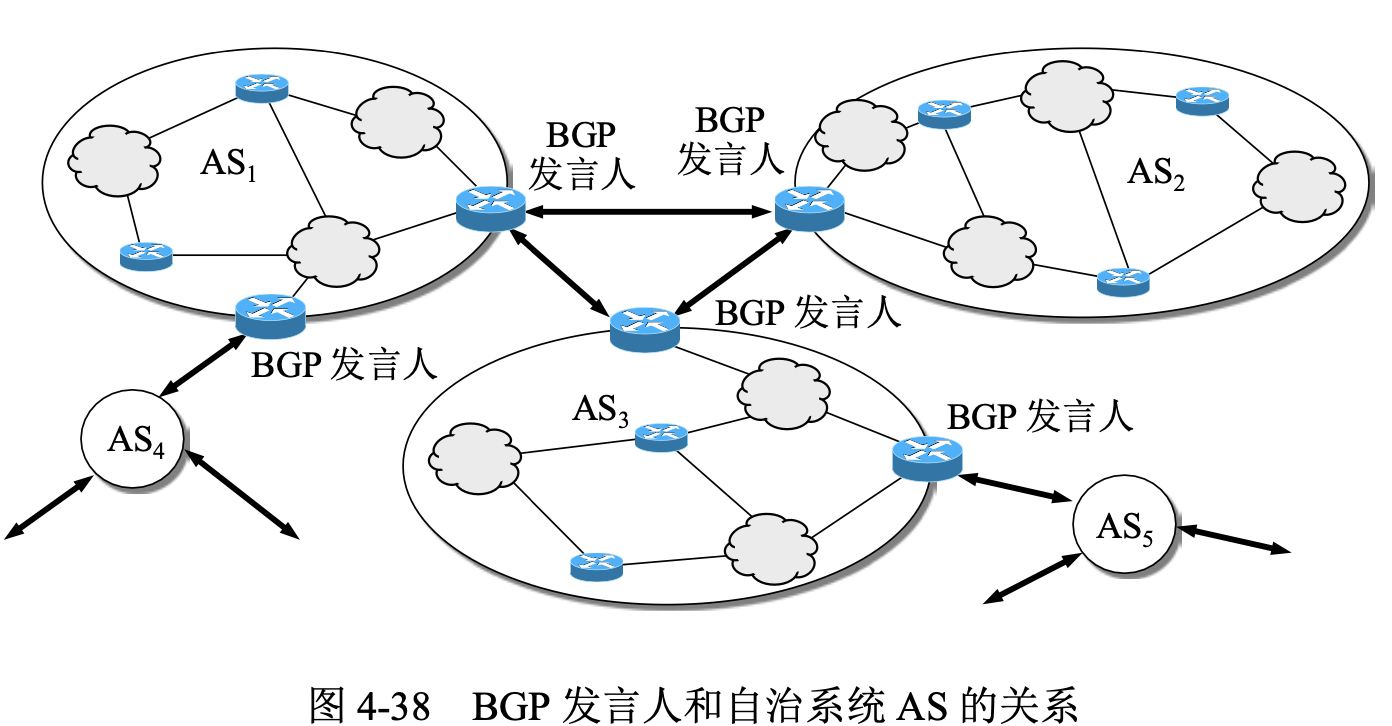
\includegraphics[width=0.7\textwidth]{img/4.38}
	\end{figure}

	\begin{itemize}
		\item 当 BGP 发言人互相交换例网络可达性的信息后,各 BGP 发言人就根据所采用的策略从收到的路由信息中找出到达各自治系统的较好的路由,也就是构造出树形结构、不存在回路的自治系统连通图
	\end{itemize}

	\begin{figure}[H]
		\centering
		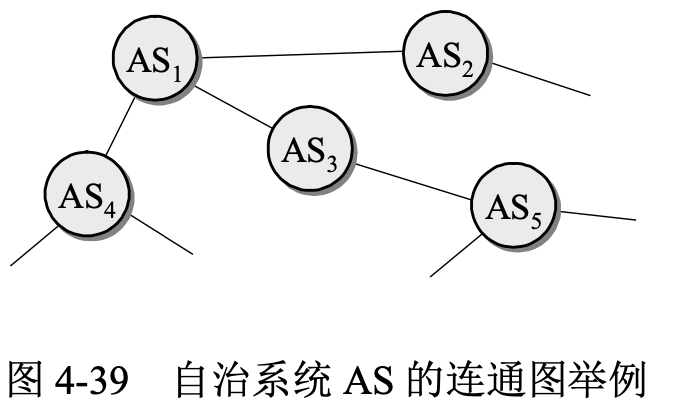
\includegraphics[width=0.4\textwidth]{img/4.39}
	\end{figure}

	\begin{itemize}
		\item BGP 适用于多级结构的因特网,以下图为例:
		\begin{itemize}
			\item 自治系统 $AS_2$ 的 BGP 发言人通知主干网的BGP发言人:“要到达网络$N_1$,$N_2$,$N_3$ 和$N_4$可经过$AS_2$。”
			\item 主干网在收到这个通知后,就发出通知:“要到达网络$N_1$,$N_2$,$N_3$ 和 $N_4$ 可沿路径 $(AS_1,AS_2)$。”
			\item 同理,主干网还可发出通知:“要到达网络 $N_5$,$N_6$ 和 $N_7$ 可沿路径 $(AS_1,AS_3)$。”
		\end{itemize}
	\end{itemize}

	\begin{figure}[H]
		\centering
		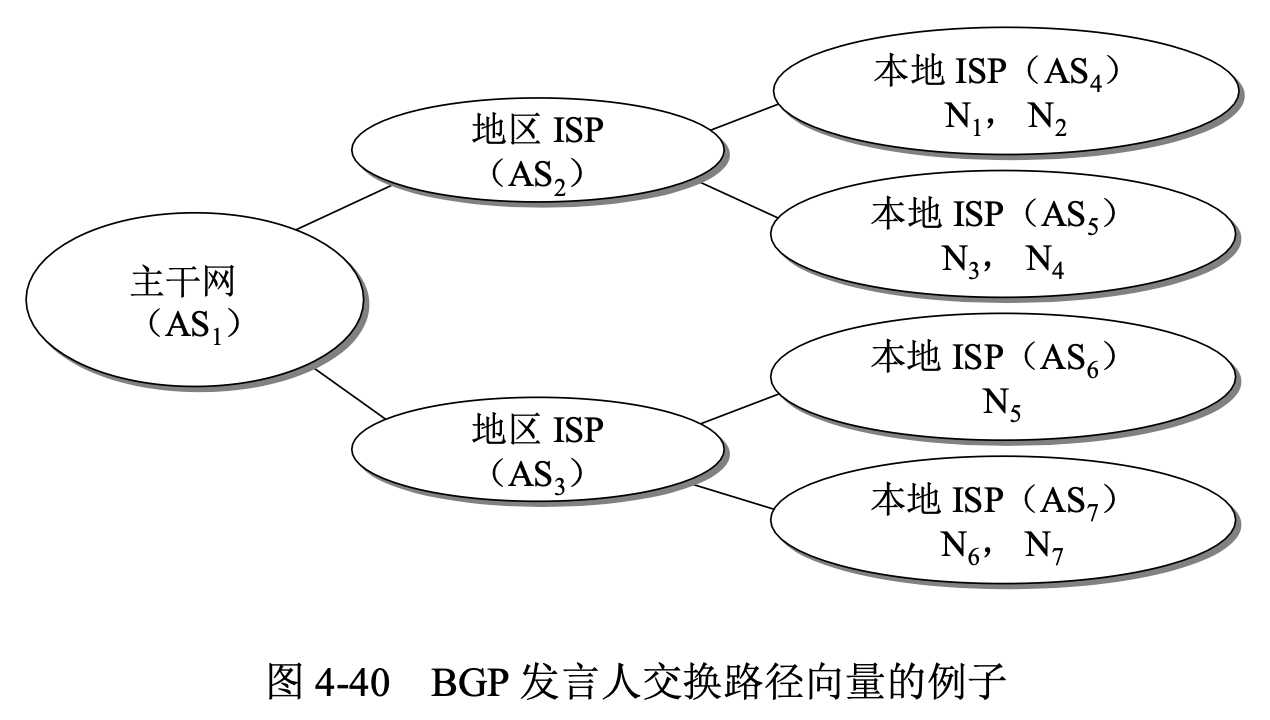
\includegraphics[width=0.55\textwidth]{img/4.40}
	\end{figure}

	\begin{itemize}
		\item BGP 有以下四种报文:
		\begin{itemize}
			\item OPEN(打开)报文,用来与相邻的另一个 BGP 发言人建立关系,使通信初始化
			\item UPDATE(更新)报文,用来通告某一路由的信息,以及列出要撤销的多条路由
			\item KEEPALIVE(保活)报文,用来周期性地证实邻站的连通性
			\item NOTIFICATION(通知)报文,用来发送检测到的差错
		\end{itemize}
	\end{itemize}

	\begin{figure}[H]
		\centering
		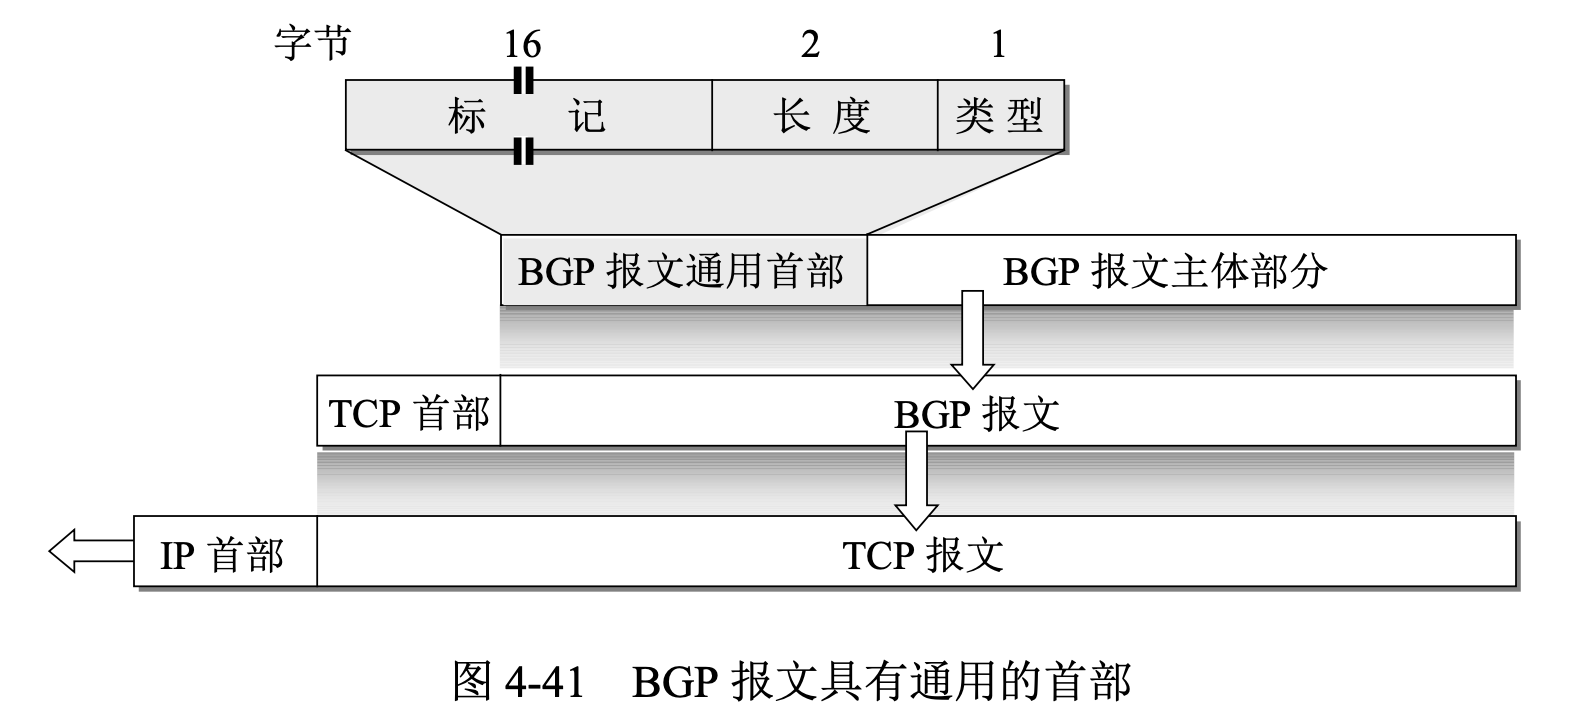
\includegraphics[width=0.65\textwidth]{img/4.41}
	\end{figure}

	\subsection{路由器的构成}

	\subsubsection{路由器的结构}

	\begin{itemize}
		\item 路由器是一种具有多个输入端口和多个输出端口的专用计算机,其任务是转发分组
		\item 从路由器某个输入端口收到的分组,按照分组要去的目的地(即目的网络),把该分组从路由器的某个合适的输出端口转发给下一跳路由器。下一跳路由器也按照这种方法处理分组, 直到该分组到达终点为止
	\end{itemize}
	\begin{figure}[H]
		\centering
		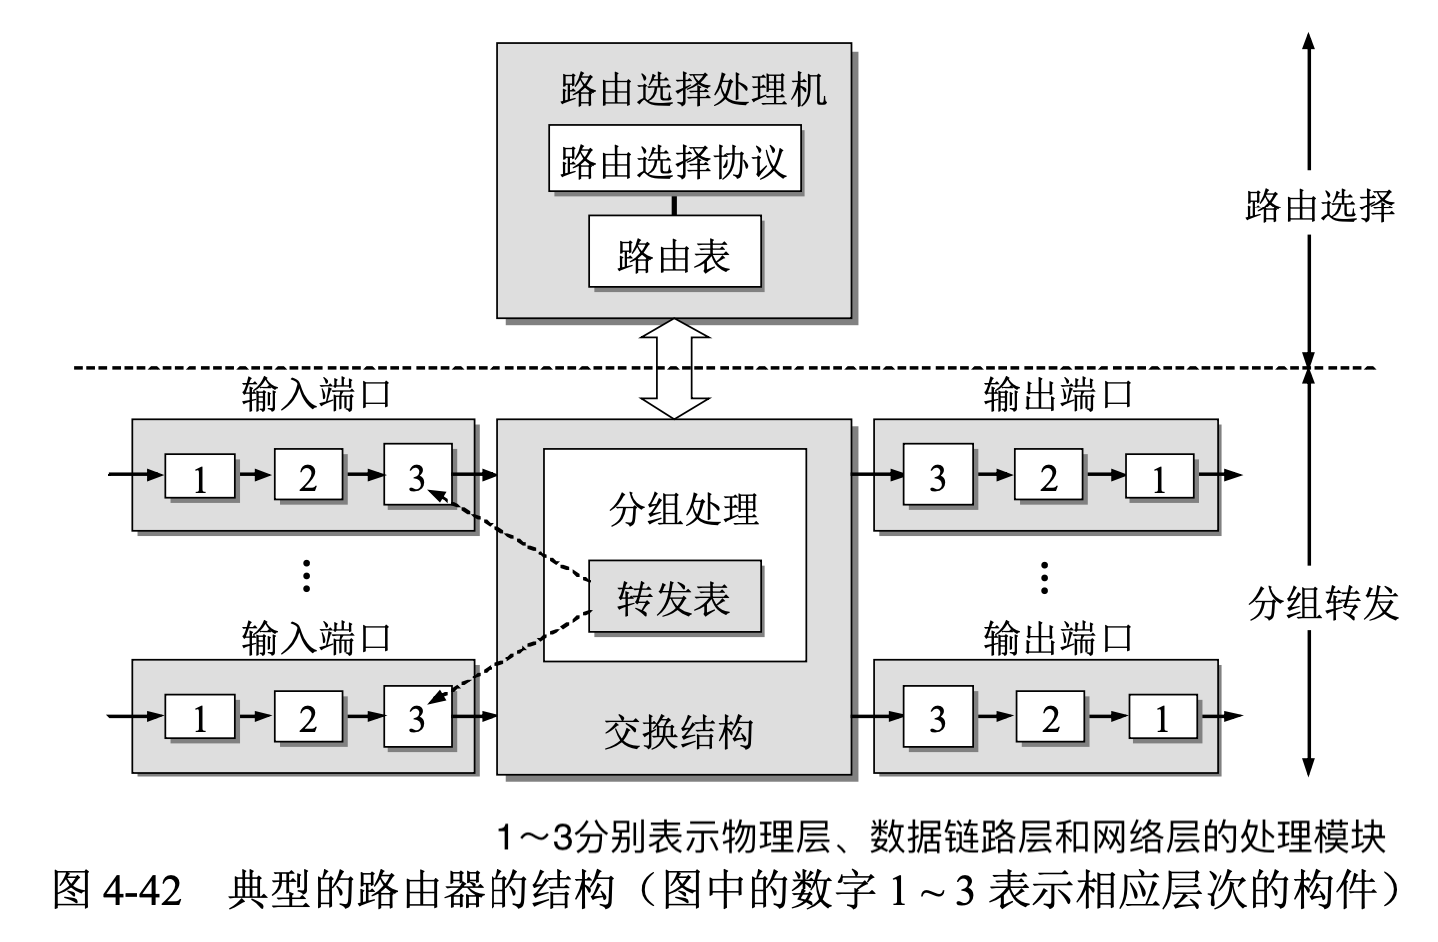
\includegraphics[width=0.7\textwidth]{img/4.42}
	\end{figure}

	整个的路由器结构可划分为两大部分:路由选择部分和分组转发部分
	\begin{itemize}
		\item 路由选择部分也叫做控制部分,其核心构件是路由选择处理机
		\begin{itemize}
			\item 路由选择处理机的任务是根据所选定的路由选择协议构造出路由表,同时经常或定期地和相邻路由器交换路由信 息而不断地更新和维护路由表
		\end{itemize}
		\item 分组转发部分由三部分组成:交换结构、一组输入端口和一组输出端口
		\begin{itemize}
			\item 交换结构(switching fabric)又称为交换组织,它的作用就是根据转发表\footnote{注意,在讨论路由选择的原理时,往往不去区分转发表和路由表的区别,而可以笼统地都使用路由表这一名词}
			(forwarding table)对分组进行处理,将某个输入端口进入的分组从一个合适的输出端口转发出去
			\item 输入端口中的查找和转发功能在路由器的交换功能中是最重要的。为了使交换功能分散化,往往把复制的转发表放在每一个输入端口中(如上图中的虚线箭头所示)。路由选择处理机负责对各转发表的副本进行更新。这些副本常称为“影子副本”
			\item 分组在路由器的输入端口和输出端口都可能会在队列中排队等候处理
		\end{itemize}
	\end{itemize}

	\begin{figure}[H]
		\centering
		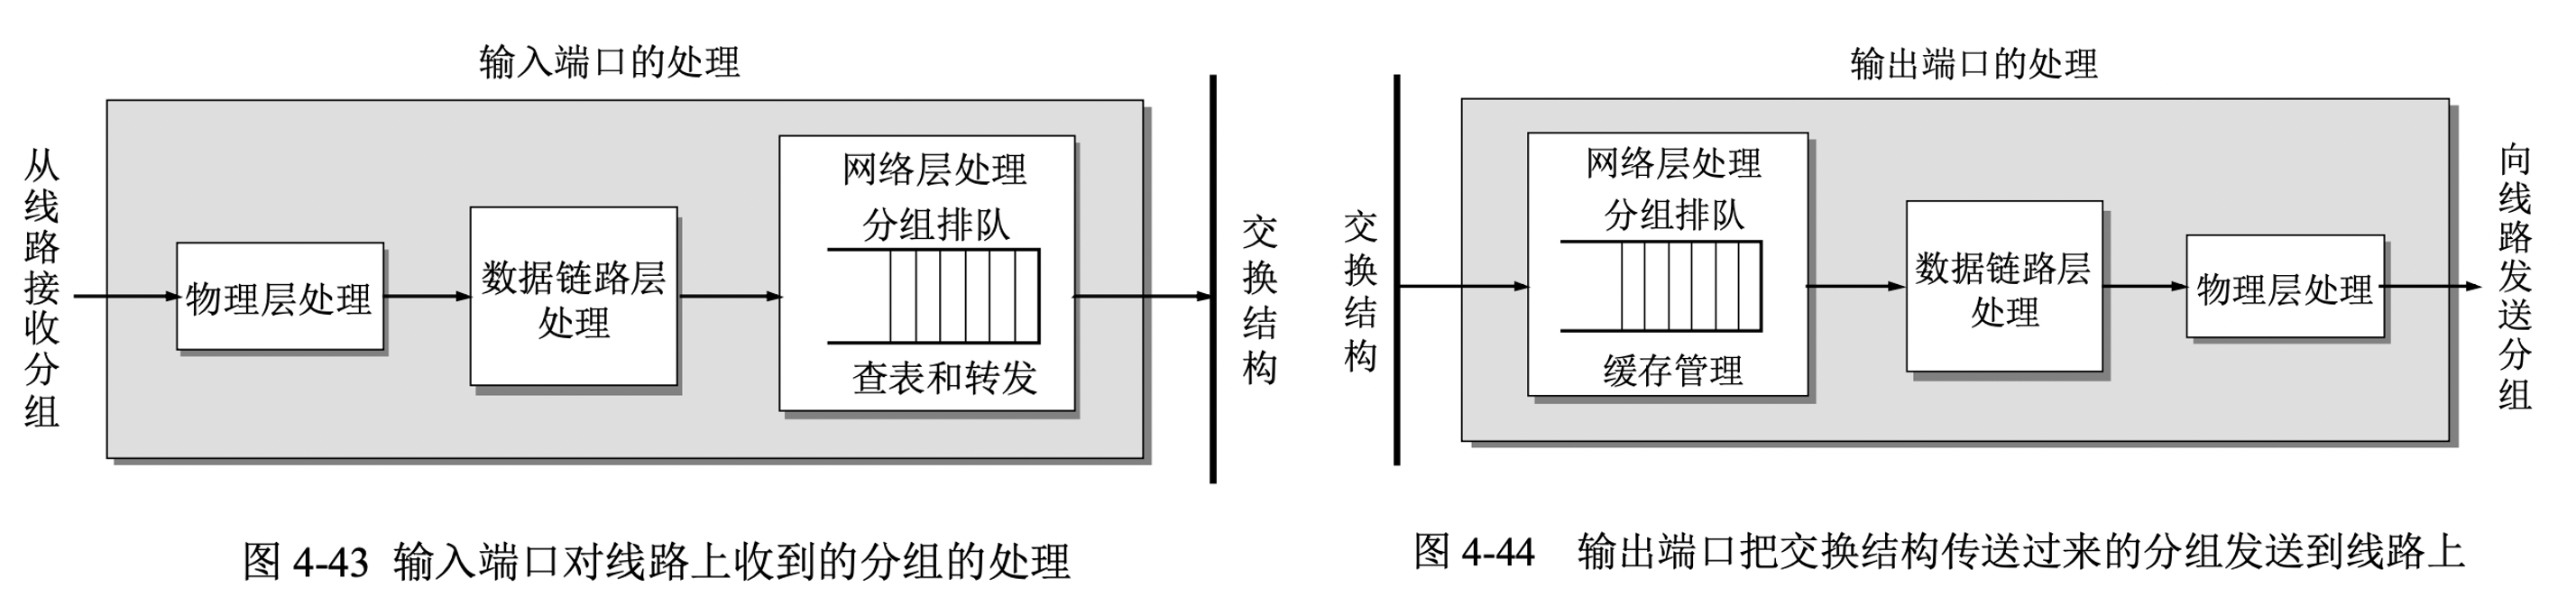
\includegraphics[width=0.75\textwidth]{img/4.43}
	\end{figure}

	\subsubsection{交换结构}
	\begin{figure}[H]
		\centering
		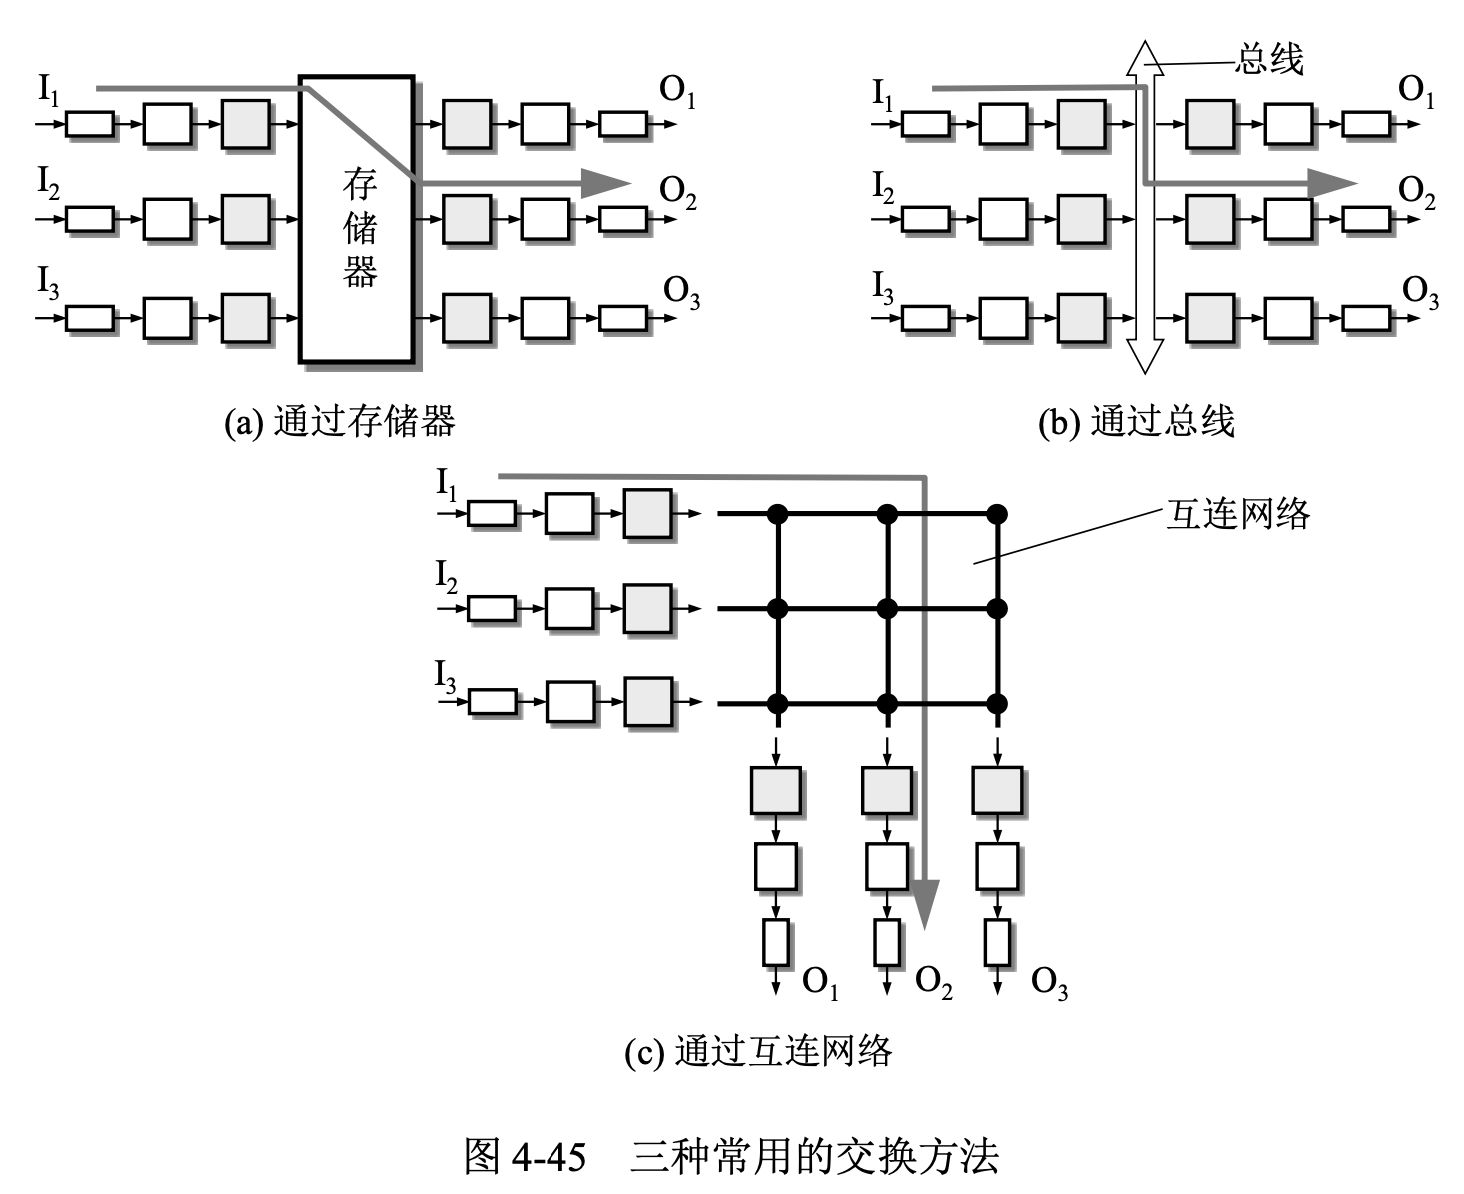
\includegraphics[width=0.7\textwidth]{img/4.45}
	\end{figure}

	\begin{itemize}
		\item 最早使用的路由器就是利用普通的计算机,用计算机的 CPU 作为路由器的路由选择 理机。路由器的输入和输出端口的功能和传统的操作系统中的 I/O 设备一样
		\item 许多现代的路由器也通过存储器进行交换,上图(a)表示分组通过存储器进行交换。与早期的路由器的区别就是,目的地址的查找和分组在存储器中的缓存都是在输入端口中进行的
		\item 图 (b)是通过总线进行交换的示意图。采用这种方式时,数据报从输入端口通过共享的总线直接传送到合适的输出端口,而不需要路由选择处理机的干预。但是,由于总线是共享的,因此在同一时间只能有一个分组在总线上传送。当分组到达输入端口时若发现总线忙,则被阻塞而不能通过交换结构,并在输入端口排队等待。因为每一个要转发的分组都要通过这一条总线,因此路由器的转发带宽就受总线速率的限制
		\item 图(c)是通过纵横交换结构进行交换。这种交换机构常称为互连网络,它有 $2N$ 条总线,可以使 $N$ 个输入端口和 $N$ 个输出端口相连接,这取决于相应的交叉结点是使水平总线和垂直总线接通还是断开。当输入端口收到一个分组时,就将它发送到与该输入端口相连的水平总线上。若通向所要转发的输出端口 的垂直总线是空闲的,则在这个结点将垂直总线与水平总线接通,然后将该分组转发到这个输出端口。但若该垂直总线已被占用,则后到达的分组就被阻塞,必须在输入端口排队
	\end{itemize}

	\section{虚拟专用网VPN和网络地址转换NAT}

	\subsection{虚拟专用网VPN}
	\begin{itemize}
		\item 2013 年,RFC 6890全面地给出了一些专用地址,这些地址只能用于一个机构的内部通信,而不能用于和互联网上的主机通信,采用这样专用 IP 地址的互连网络称为专用网,这些地址为
		\begin{itemize}
			\item 10.0.0.0 到 10.255.255.255(10.0.0.0/8)
			\item 172.16.0.0 到 172.31.255.255(172.16.0.0/12)
			\item 192.168.0.0 到 192.168.255.255(192.168.0.0/16)
		\end{itemize}
		\item 利用公用的因特网作为本机构各专用网之间的通信载体,这样的专用网又称为虚拟专用网(virtual private network)
		\item 由于 IPv4 地址的紧缺,一个机构能够申请到的 IPv4 地址数量往往远小于本机构所拥有的主机数量。因此,虚拟专用网中的各主机所分配的地址应该是本机构可自由分配的专用地址,而不是需要申请的、在因特网上使用的共有地址
	\end{itemize}

	\begin{figure}[H]
		\centering
		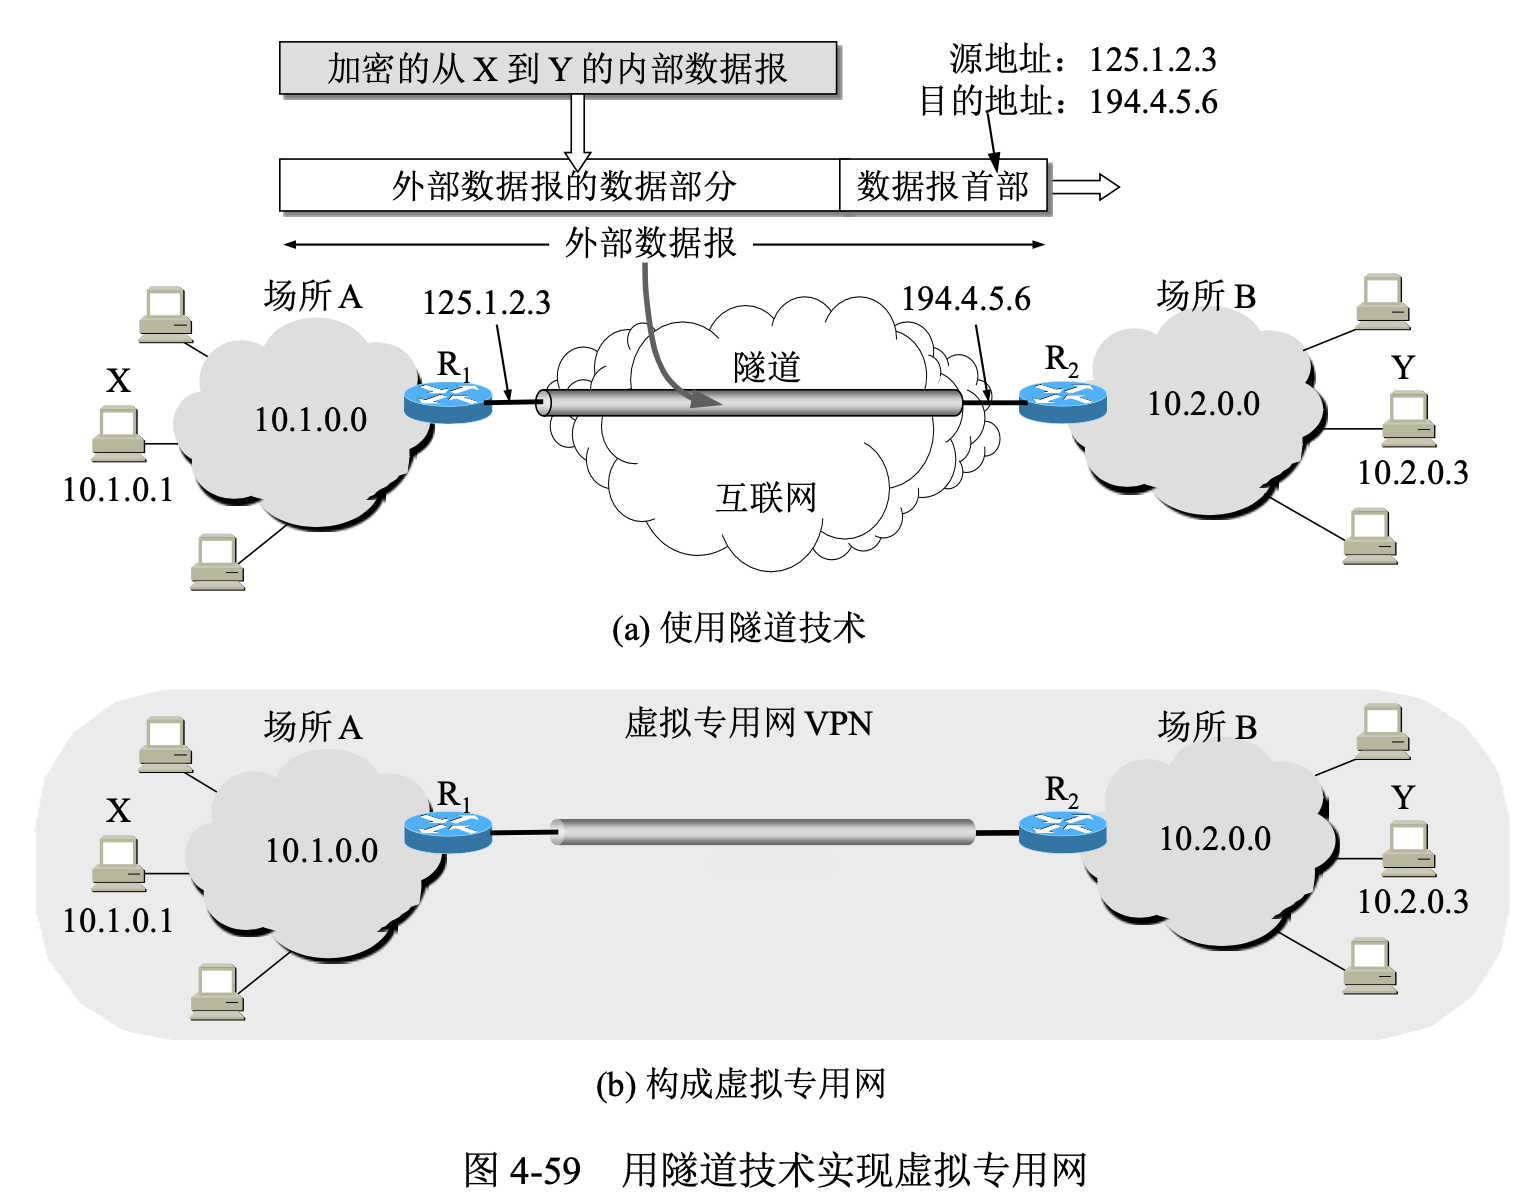
\includegraphics[width=0.7\textwidth]{img/4.59}
	\end{figure}

	\subsection{网络地址转换NAT}
	\begin{itemize}
		\item 虽然因特网采用了无分类编址方式来缓解 IPv4 地址空间耗尽的速度,但由于因特网用户数目的激增,特别是大量小型办公室网络和家庭网络接入因特网的需求不断增加,IPv4 地址空间即将面临耗尽的危险仍然没有被解除
		\item 1994 年提出了一种网络地址转换 NAT 的方法再次缓解了 IPv4 地址空间即将耗尽的问题
		\item NAT 能使大量使用内部专用地址的专用网络用户共享少量外部全球地址来访问因特网上的主机和资源
	\end{itemize}

	\begin{figure}[H]
		\centering
		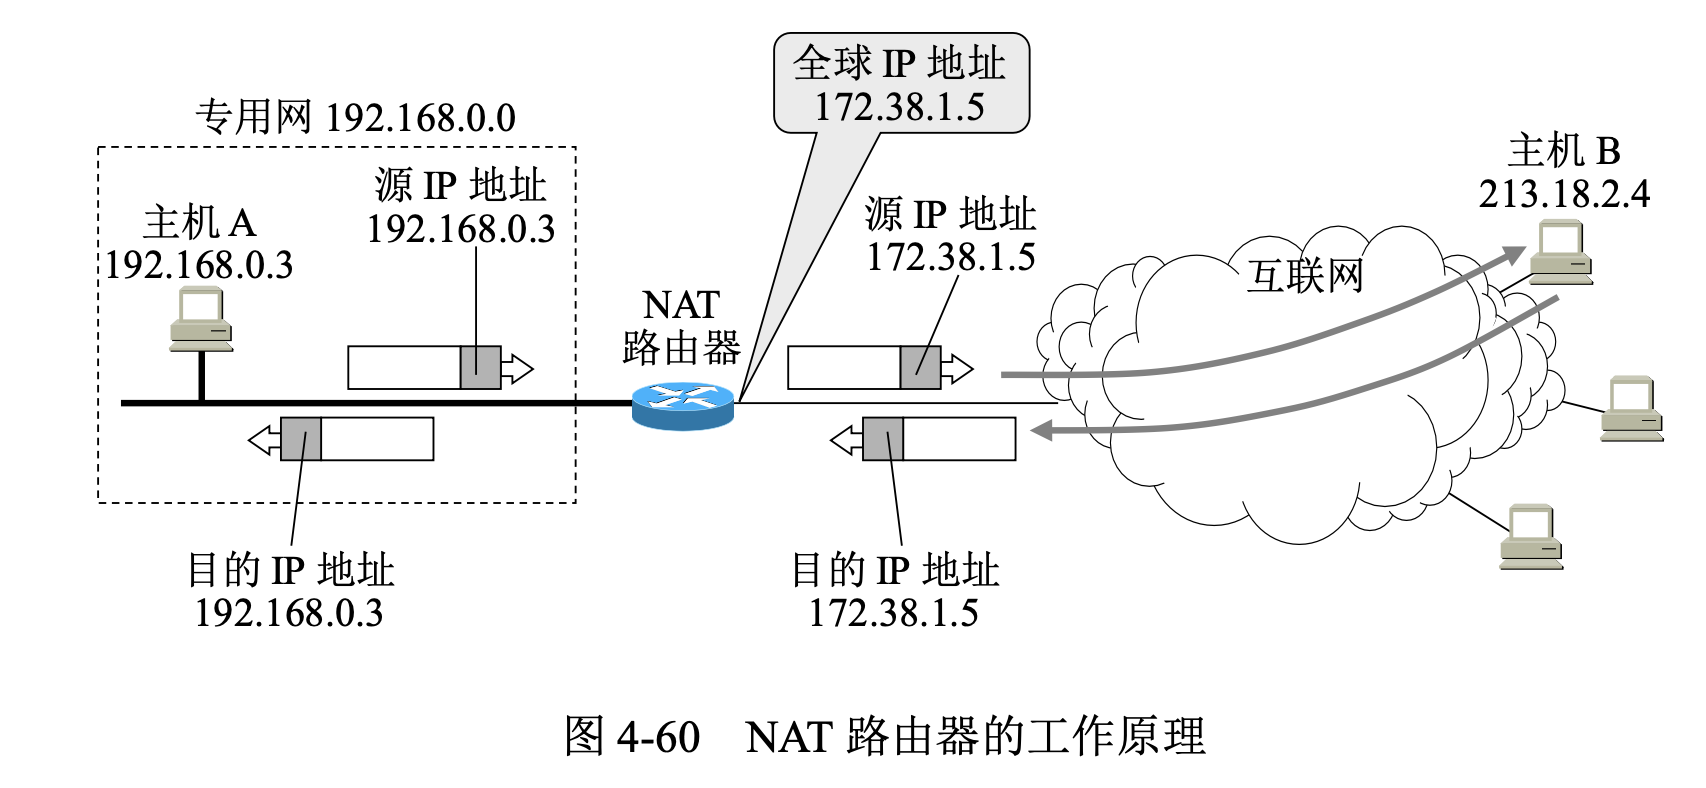
\includegraphics[width=0.7\textwidth]{img/4.60}
	\end{figure}

	NAT 路由器工作原理
	\begin{itemize}
		\item 
		\begin{sloppypar}
			NAT 路由器收到从专用网内部的主机 A 发往互联网上主机 B 的 IP 数据报:源 IP 地址是 192.168.0.3,而目的 IP 地址是 213.18.2.4。NAT 路由器把 IP 数据报的源 IP 地址 192.168.0.3,转换为新的源 IP 地址(即 NAT 路由器的全球 IP 地址)172.38.1.5,然后转发出去
		\end{sloppypar}
		\item 主机 B 收到这个 IP 数据报时,以为 A 的 IP 地址是 172.38.1.5。当 B 给 A 发送应答时,IP 数据报的目的 IP 地址是 NAT 路由器的 IP 地址 172.38.1.5
		\item 当 NAT 路由器收到互联网上的主机 B 发来的 IP 数据报时,还要进行一次 IP 地址的转换。通过 NAT 地址转换表,就可把 IP 数据报上的旧的目的 IP 地址 172.38.1.5,转换为新的目的 IP 地址 192.168.0.3(主机 A 真正的本地 IP 地址)
		\item 该过程的 NAT 地址转换表如下
	\end{itemize}

	\begin{table}[H]
		\centering
		\begin{tabular}{|c|c|c|c|}
		\hline
		方向 & 字段       & 旧的 IP 地址    & 新的 IP 地址    \\ \hline
		出  & 源 IP 地址  & 192.168.0.3 & 172.38.1.5  \\ \hline
		入  & 目的 IP 地址 & 172.38.1.5  & 192.168.0.3 \\ \hline
		出  & 源 IP 地址  & 192.168.0.7 & 172.38.1.6  \\ \hline
		入  & 目的 IP 地址 & 172.38.1.6  & 192.168.0.7 \\ \hline
		\end{tabular}
	\end{table}

	\begin{itemize}
		\item 由此可见,当 NAT 路由器具有 $n$ 个全球 IP 地址时,专用网内最多可以同时有 $n$ 台主机接入到互联网
	\end{itemize}

	由于绝大多数的网络应用都是使用运输层协议 TCP 或 UDP 来传送数据,因此可以利用运输层端口号和 IP 地址一起进行转换。这样,用一个全球 IP 地址就可以使多个拥有本地地址的主机同时和因特网上的主机通信。这种将端口号和 IP 地址一起进行转换的技术叫作网络地址与端口号转换 NAPT(network address and port translation)

	NAPT 地址转换举例

	\begin{table}[H]
		\centering
		\begin{tabular}{|c|c|c|c|}
		\hline
		方向 & 字段       & 旧的 IP 地址和端口号      & 新的 IP 地址和端口号      \\ \hline
		出  & 源 IP 地址  & 192.168.0.3:30000 & 172.38.1.5:40001  \\ \hline
		入  & 目的 IP 地址 & 172.38.1.5:30000  & 192.168.0.3:40002 \\ \hline
		出  & 源 IP 地址  & 192.168.0.7:40001 & 172.38.1.6:30000  \\ \hline
		入  & 目的 IP 地址 & 172.38.1.6:40002  & 192.168.0.7:30000 \\ \hline
		\end{tabular}
	\end{table}

	\begin{itemize}
		\item 在专用网内主机 192.168.0.3 向互联网发送 IP 数据报,其 TCP 端口号选择为 30000。NAPT 把源 IP 地址和 TCP 端口号都进行转换。另一台主机 192.168.0.4 也选择了同样的 TCP 端口号 30000。这纯属巧合。现在 NAPT 把专用网内不同的源 IP 地址都转换为同样的全球 IP 地址。但对源主机所采用的 TCP 端口号,则转换为不同的新的端口号。因此,当 NAPT 路由器收到从互联网发来的应答时,就可以从 IP 数据报的数据部分找出运输层的端口号,然后根据不同的目的端口号,从 NAPT 转换表中找到正确的目的主机
	\end{itemize}

	对于一些 P2P 网络应用,需要外网主机与内网主机进行通信,在通过 NAT 时会遇到问题,需要网络应用自己使用一些特殊的 NAT 穿越技术来解决问题

	由于 NAT 对外网屏蔽了内网主机的网络地址,能为内网的主机提供一定的安全保护

\end{document}


